\par In this chapter, the new COSY routines are benchmarked against both ICOOL and G4Beamline for pencil beams. Recall that a pencil beam is a beam with an RMS of zero for all transverse coordinates. Pencil beams are used in order to simulate a plethora of possible paths and energy losses for a particular initial condition. Both validation against past experiments and predictions of current muon ionization cooling channel efforts are also shown. Since both ICOOL and G4Beamline have automatic variable stepping, their step sizes are left as default unless explicitly stated otherwise.

\Section{Benchmark Against Other Codes}\label{sec:benchmark}

This section briefly discusses the comparison of the new COSY routines with those of two other codes, ICOOL \cite{icool} and G4Beamline \cite{g4bl}. Refer to Figures \ref{fig:100.1}--\ref{fig:400.100} (12 figures, each with three subplots) mentioned here. The benchmarking was done over both the typical momentum range of cooling channels (100, 200, 300, and 400 MeV/$c$) and various absorber lengths (1, 10, and 100 mm). These simulations were performed using a pencil beam of $5\times 10^4$ muons with the aforementioned momenta through liquid hydrogen. Note that for the transverse position and transverse momentum histograms, the absolute value of the coordinate is plotted. Therefore, the mean is not zero. For COSY, the step size was the entire absorber length. For G4Beamline in the case of a 1 mm absorber, the maximum step size was limited to 0.1 mm. This was done because of the heavy dependence of the transverse position on step size for short absorbers in G4Beamline.
\newpage
\begin{figure}[H]
  \centering
    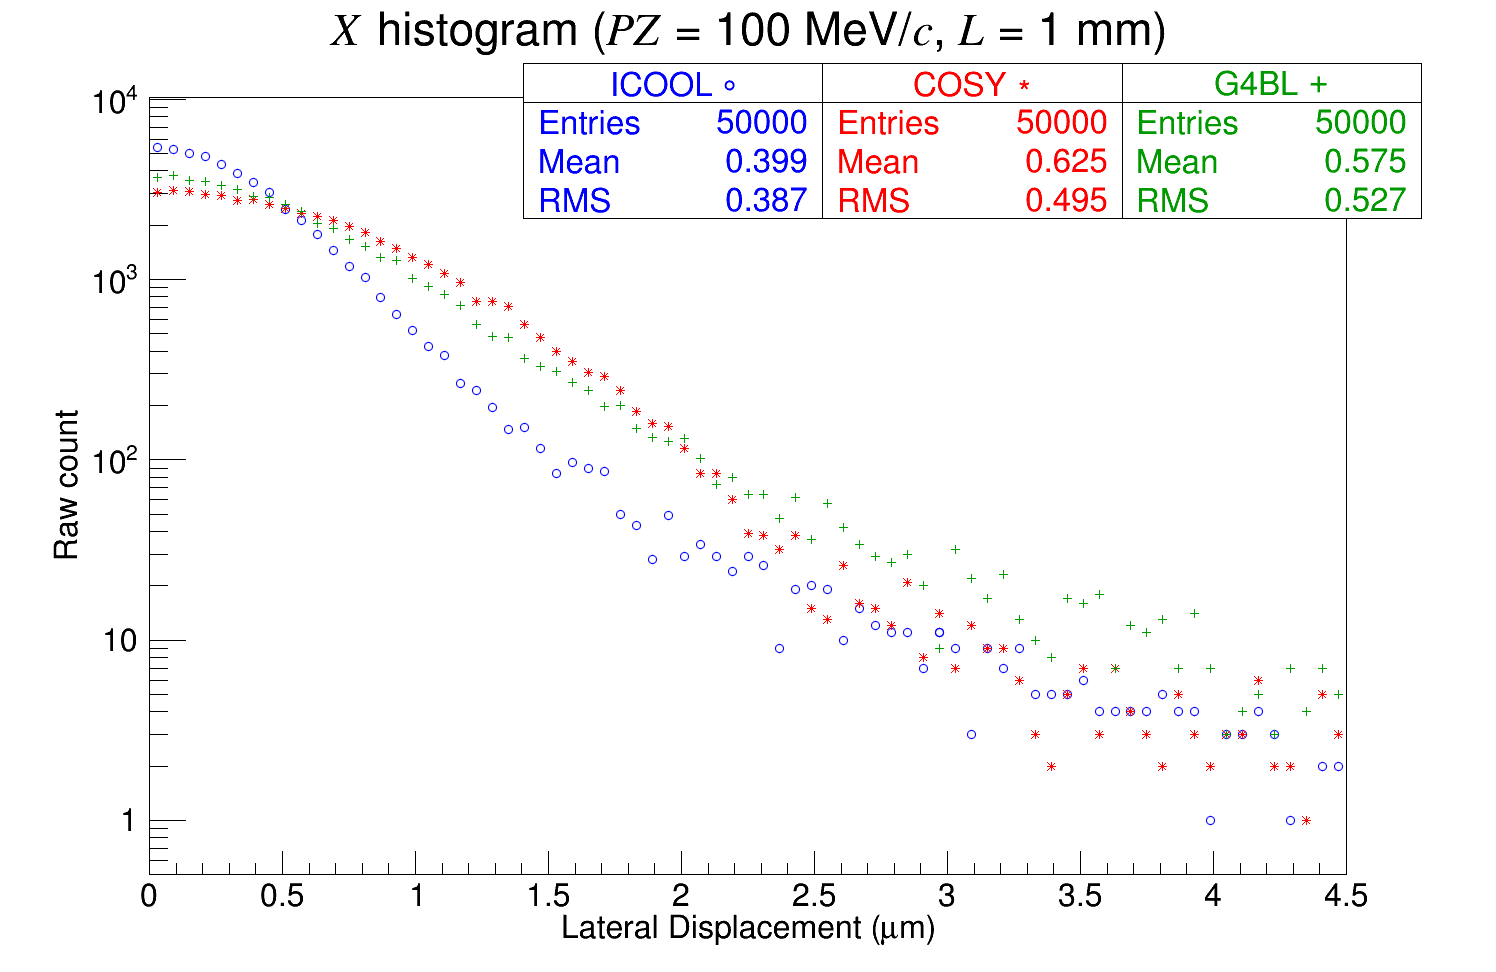
\includegraphics[width=0.7\textwidth]{Benchmarking/LH/X.100.1.png} 
    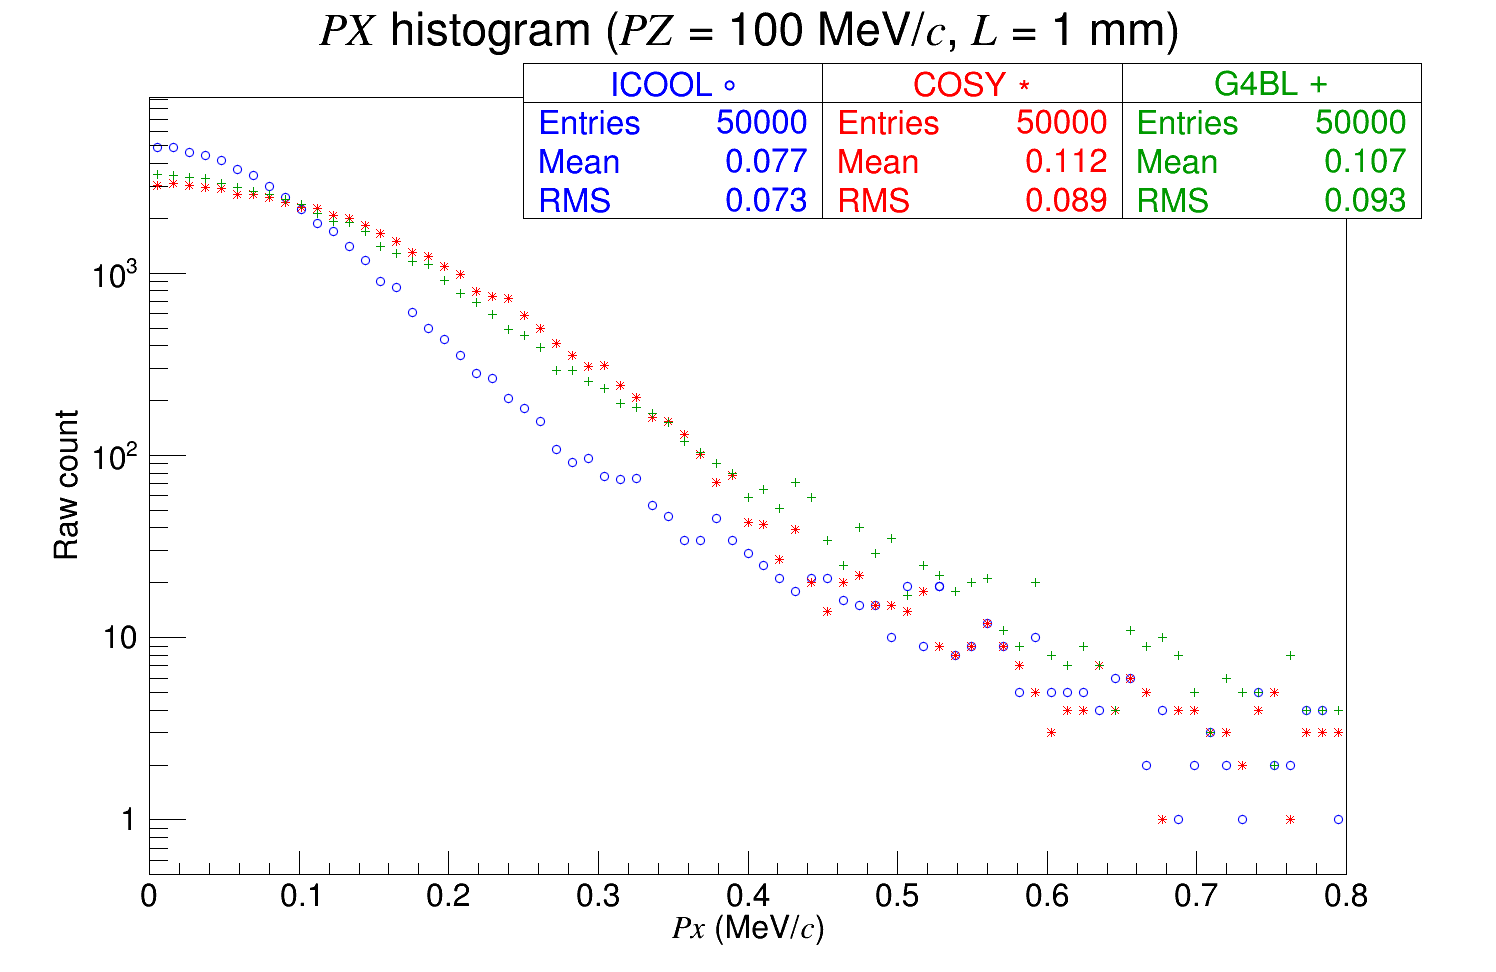
\includegraphics[width=0.7\textwidth]{Benchmarking/LH/PX.100.1.png} 
    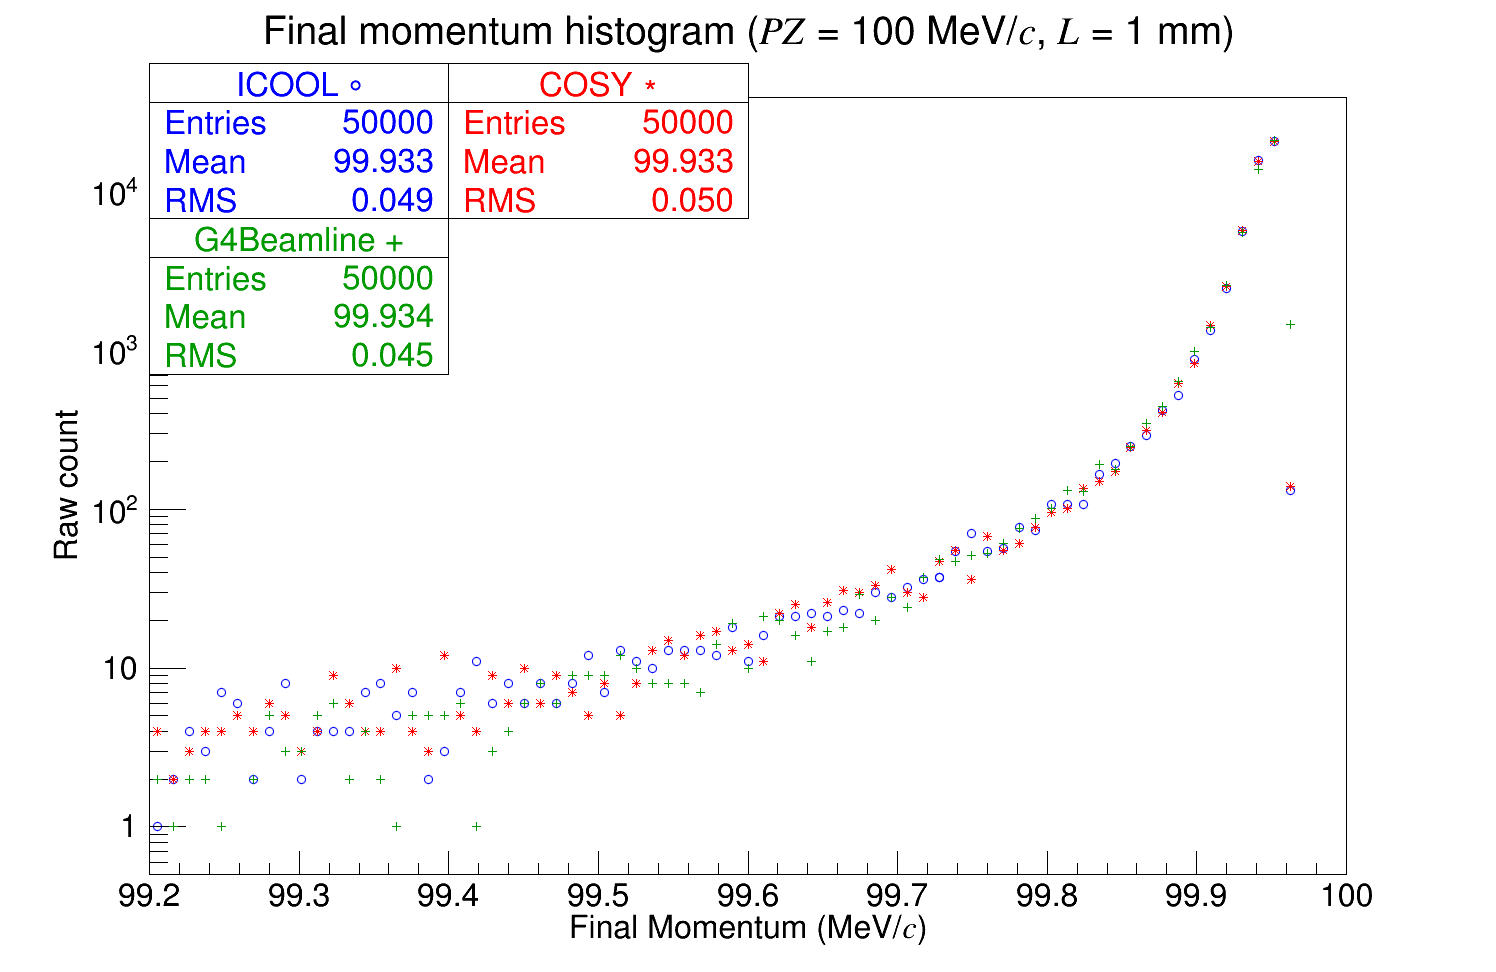
\includegraphics[width=0.7\textwidth]{Benchmarking/LH/strag.100.1.png} 
  \caption[Muons of momentum 100 MeV/$c$ through 1 mm liquid hydrogen.]{Muons of momentum 100 MeV/$c$ through 1 mm liquid hydrogen. Observe that for the $x$ and $p_x$ histograms, COSY and G4Beamline follow a Gaussian-like peak whereas ICOOL follows a Fano peak.}
  \label{fig:100.1}
\end{figure}

\begin{figure}[H]
  \centering
    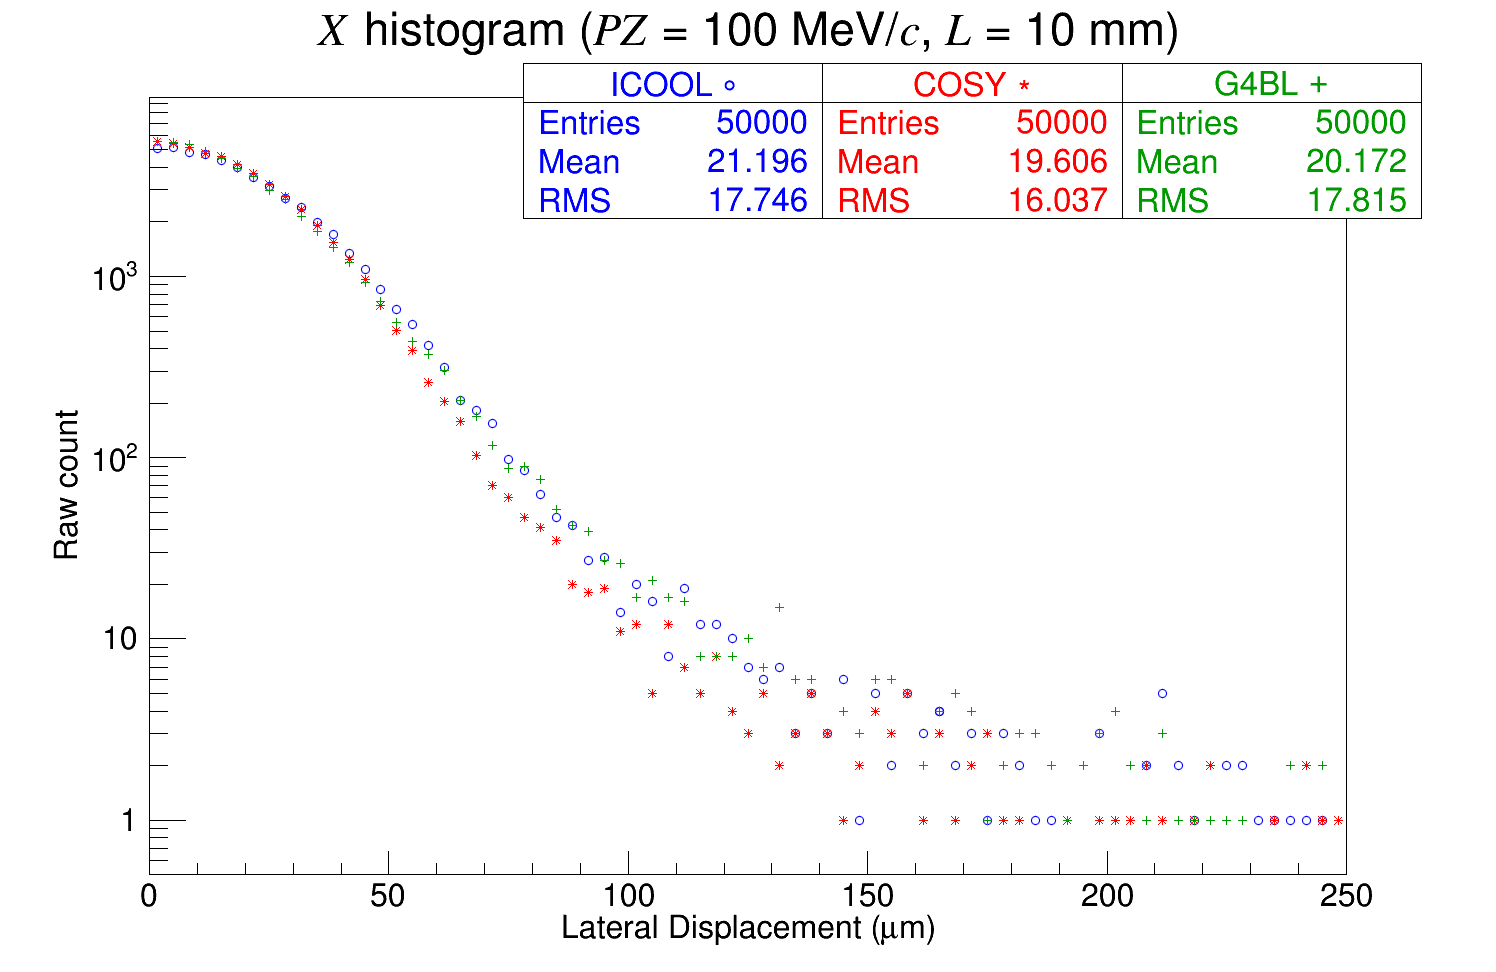
\includegraphics[width=0.7\textwidth]{Benchmarking/LH/X.100.10.png} 
    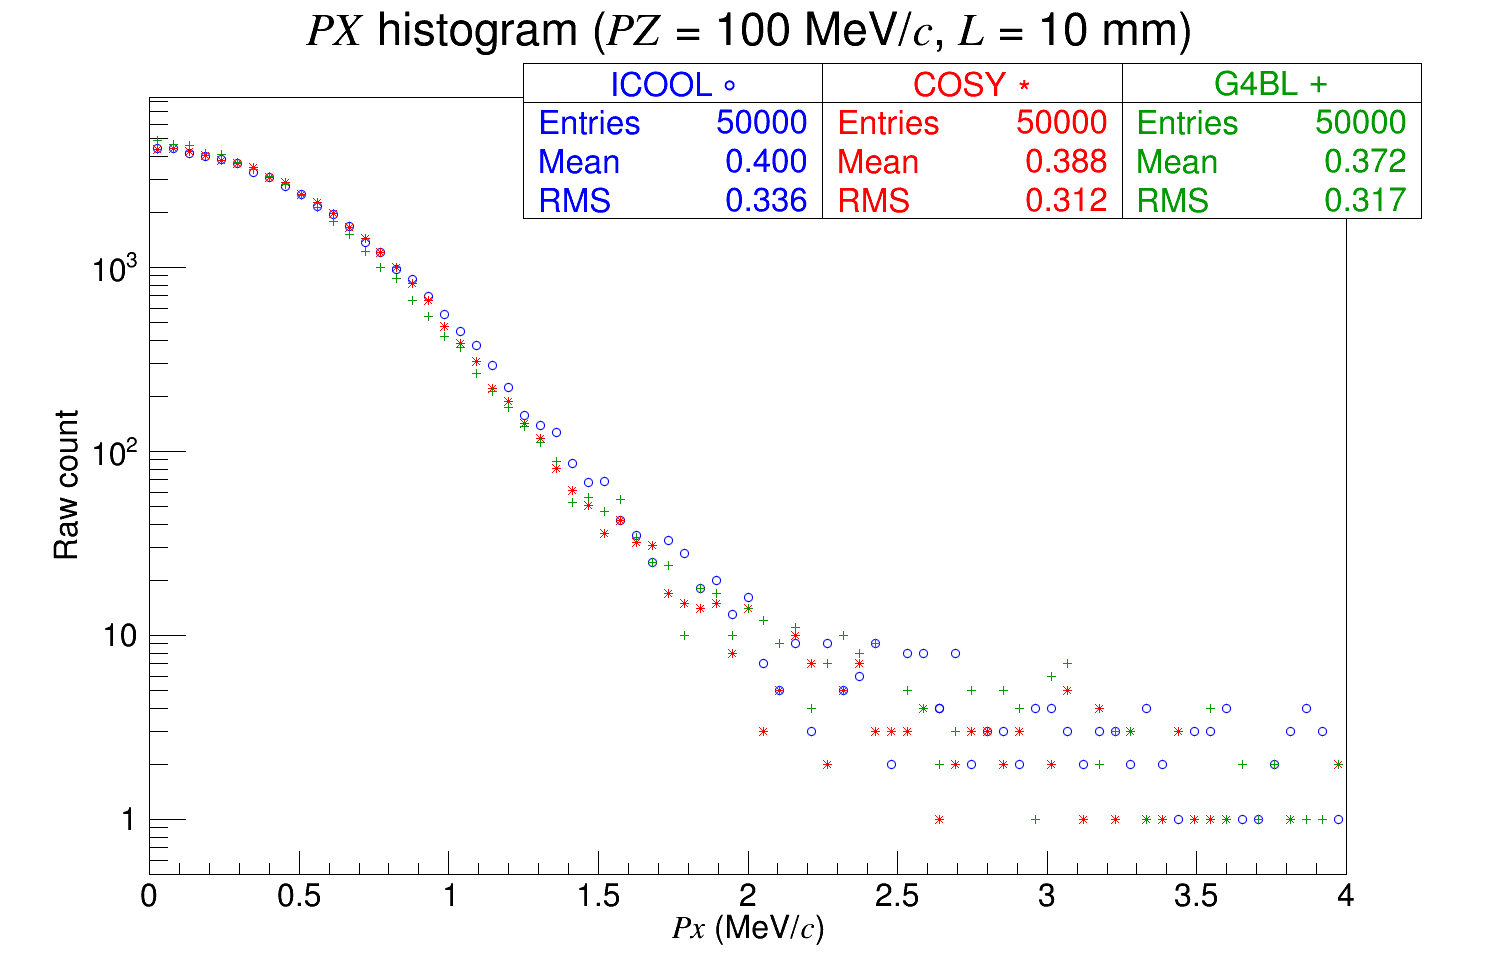
\includegraphics[width=0.7\textwidth]{Benchmarking/LH/PX.100.10.png} 
    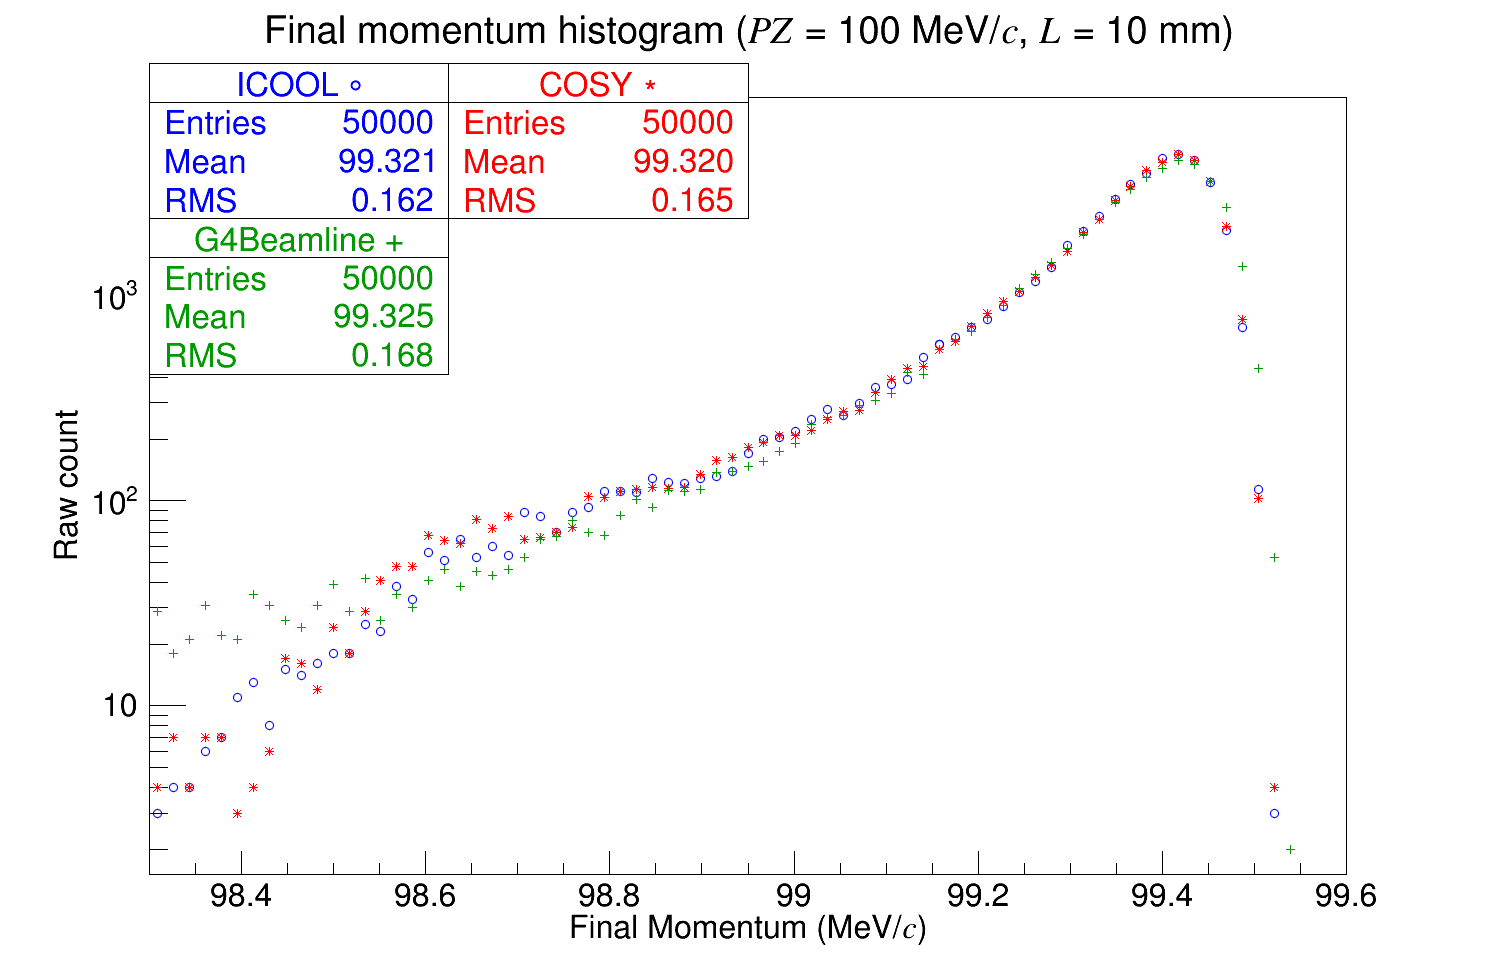
\includegraphics[width=0.7\textwidth]{Benchmarking/LH/strag.100.10.png} 
  \caption{Muons of momentum 100 MeV/$c$ through 10 mm liquid hydrogen.}
  \label{fig:100.10}
\end{figure}

\begin{figure}[H]
  \centering
    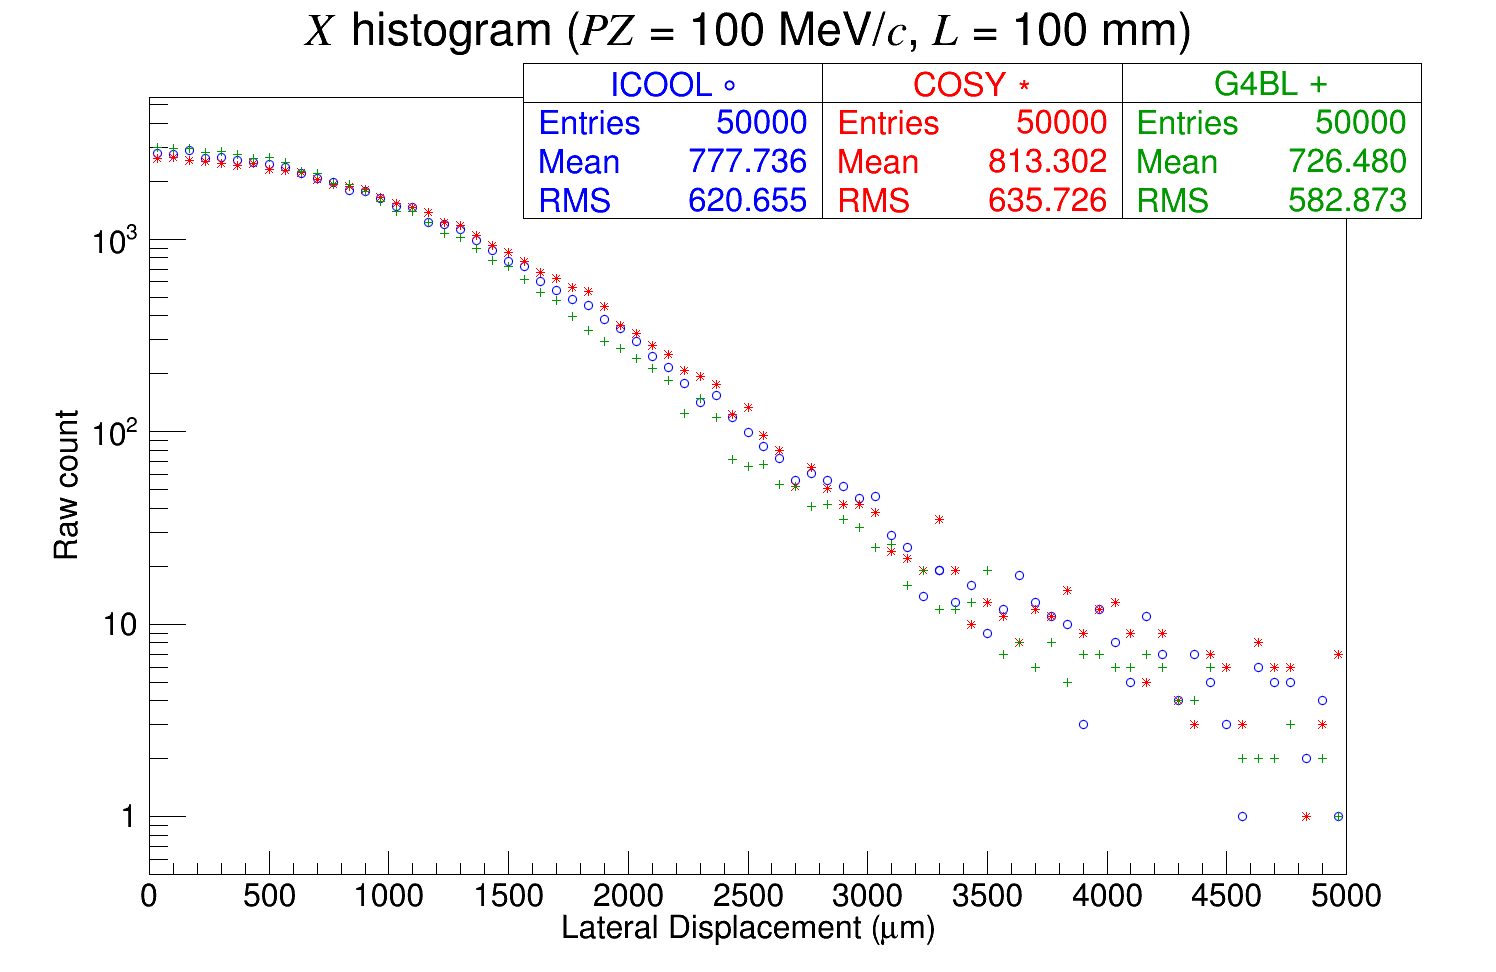
\includegraphics[width=0.7\textwidth]{Benchmarking/LH/X.100.100.png} 
    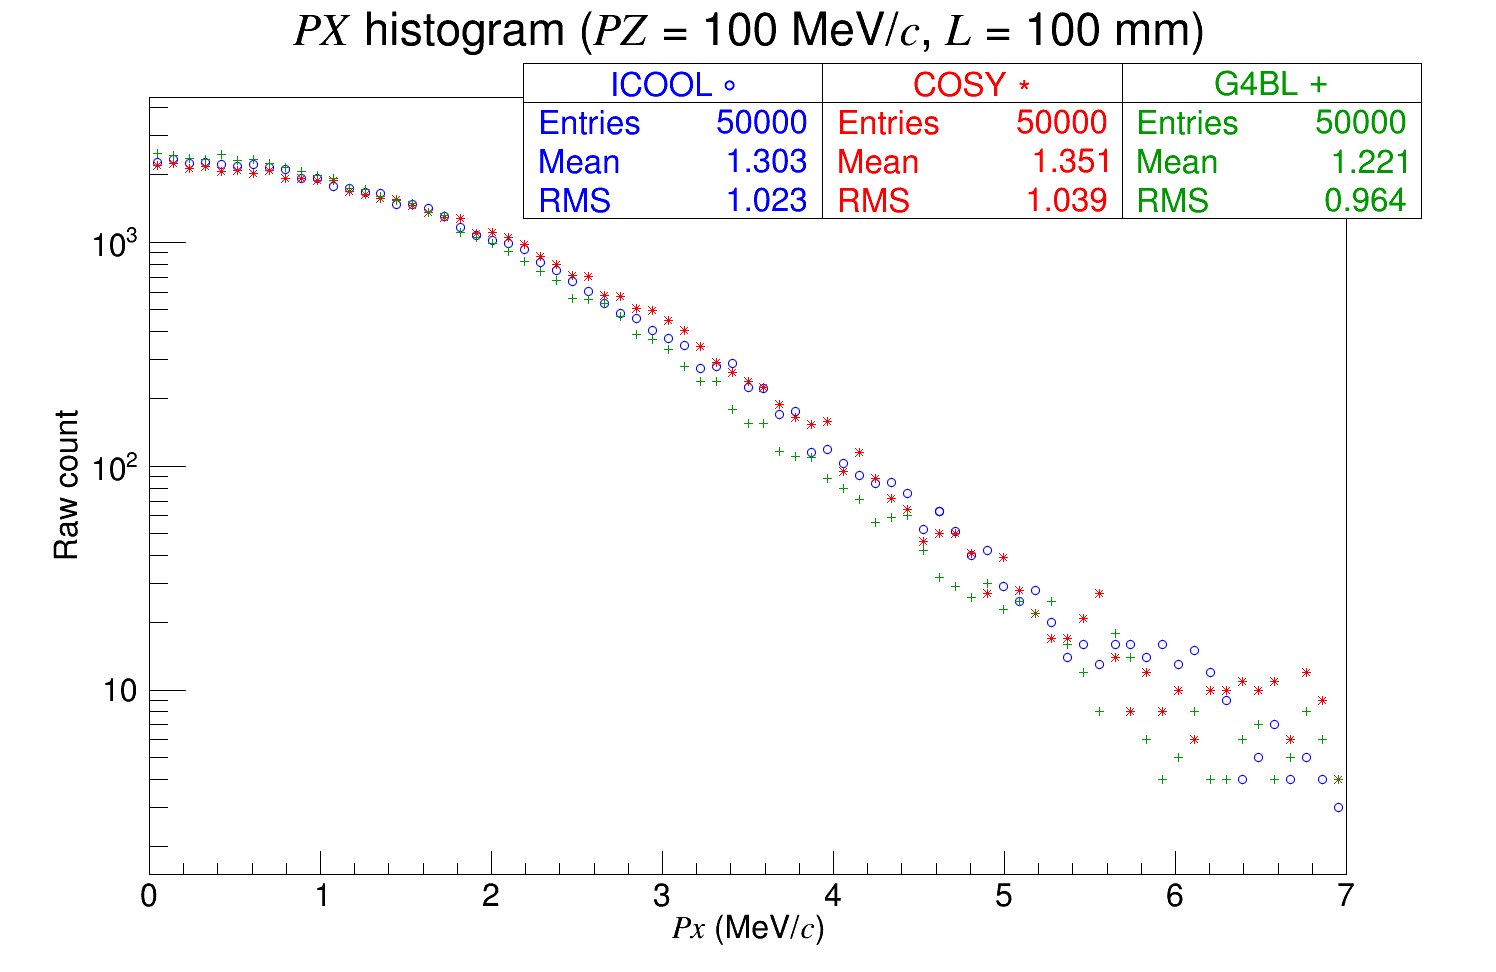
\includegraphics[width=0.7\textwidth]{Benchmarking/LH/PX.100.100.png} 
    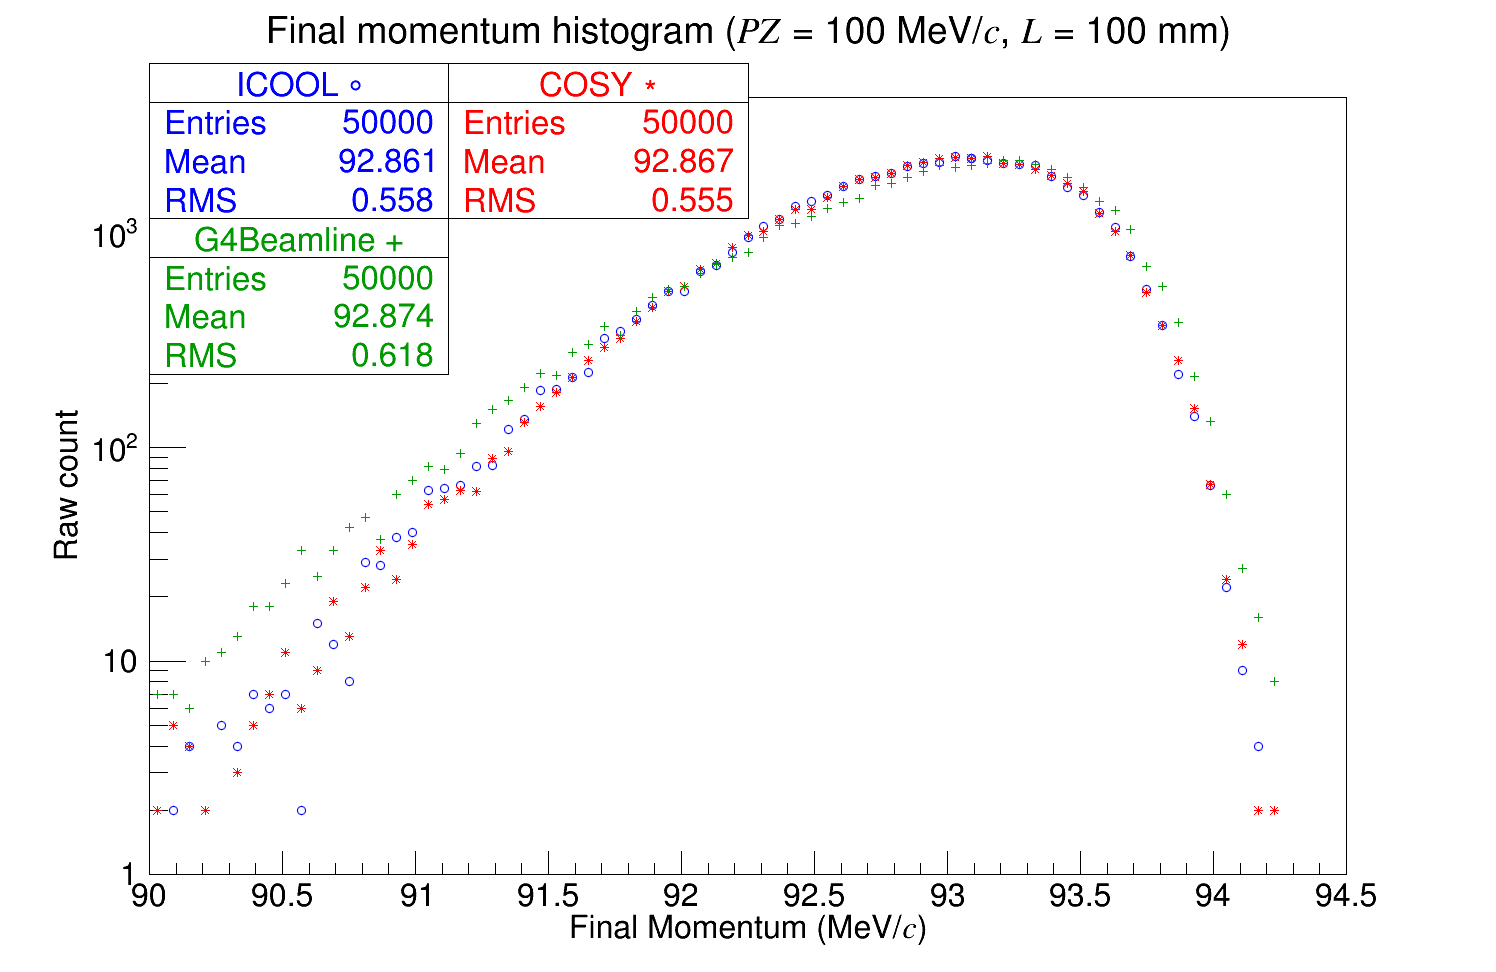
\includegraphics[width=0.7\textwidth]{Benchmarking/LH/strag.100.100.png} 
  \caption{Muons of momentum 100 MeV/$c$ through 100 mm liquid hydrogen.}
  \label{fig:100.100}
\end{figure}

\begin{figure}[H]
  \centering
    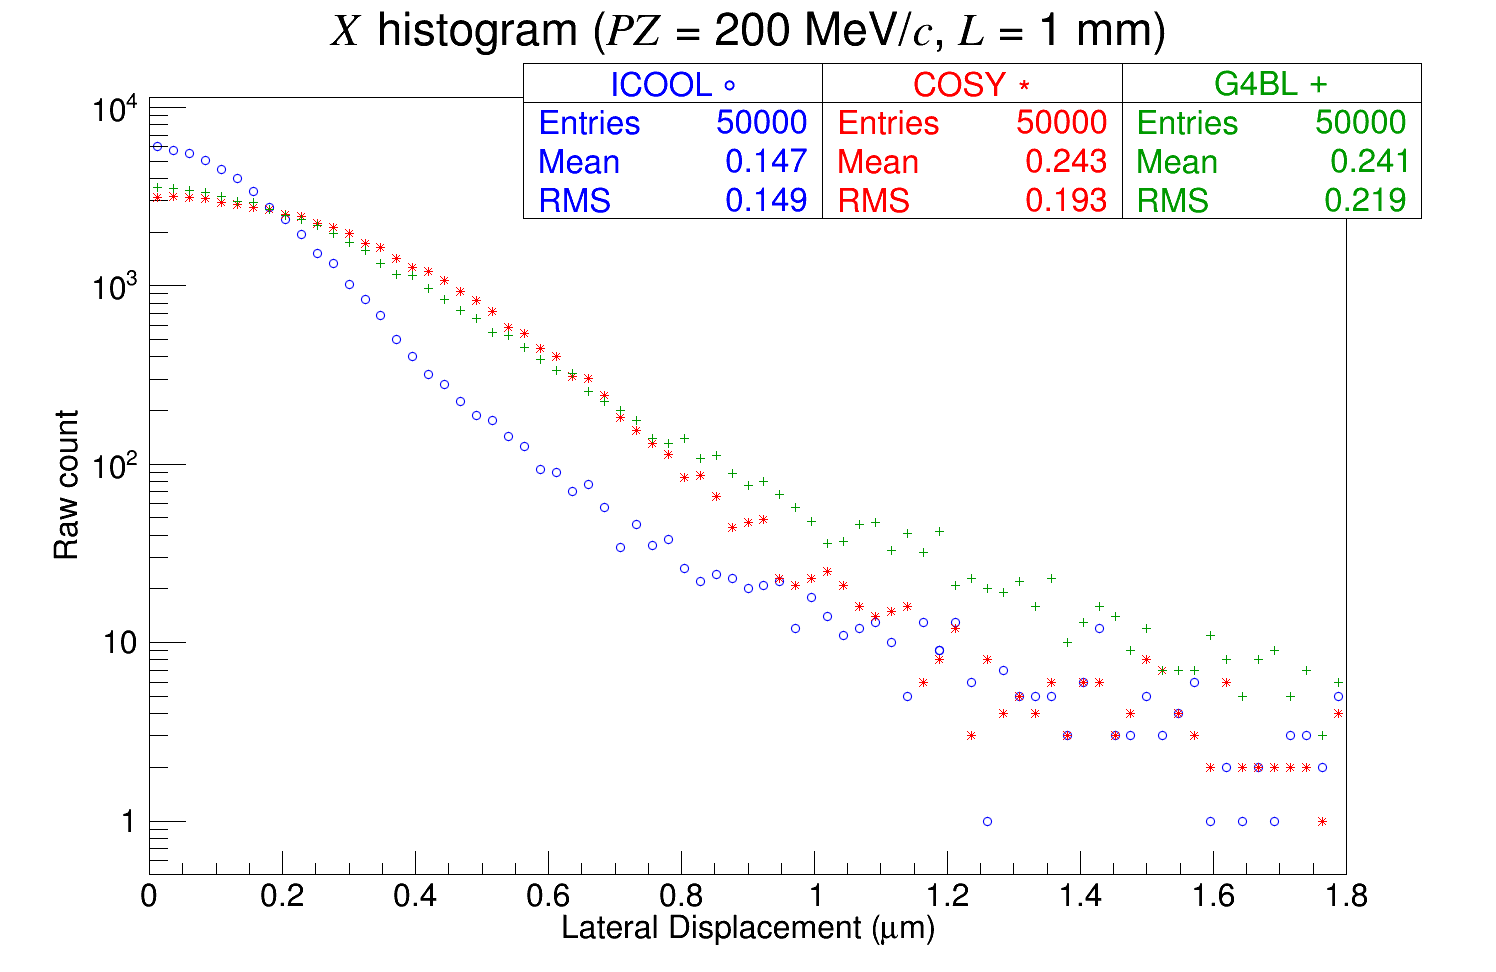
\includegraphics[width=0.7\textwidth]{Benchmarking/LH/X.200.1.png} 
    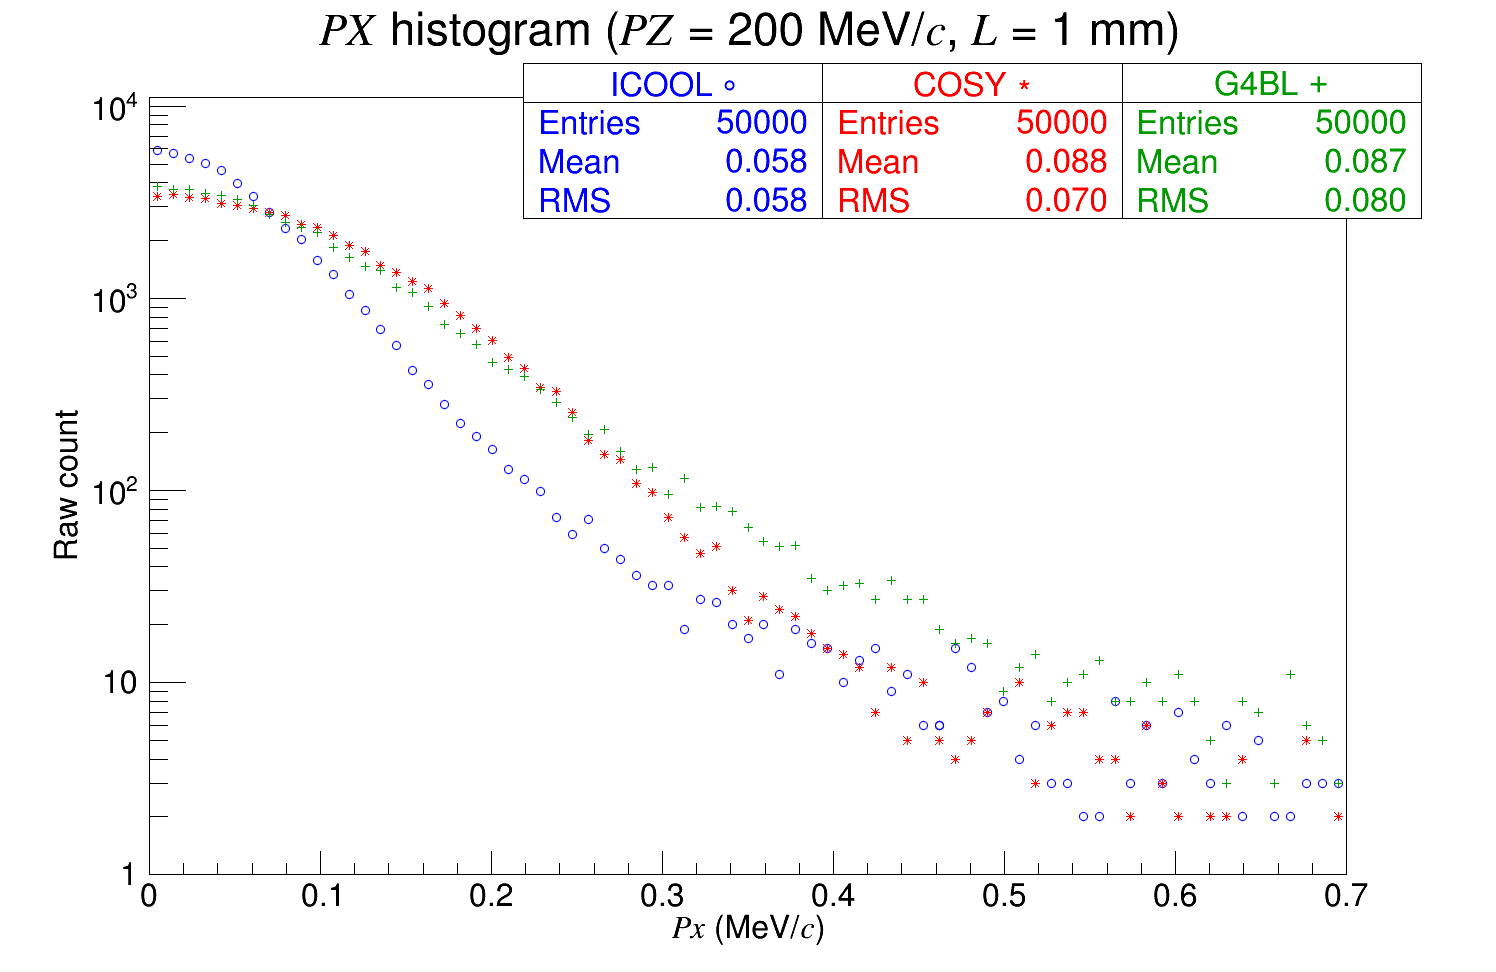
\includegraphics[width=0.7\textwidth]{Benchmarking/LH/PX.200.1.png} 
    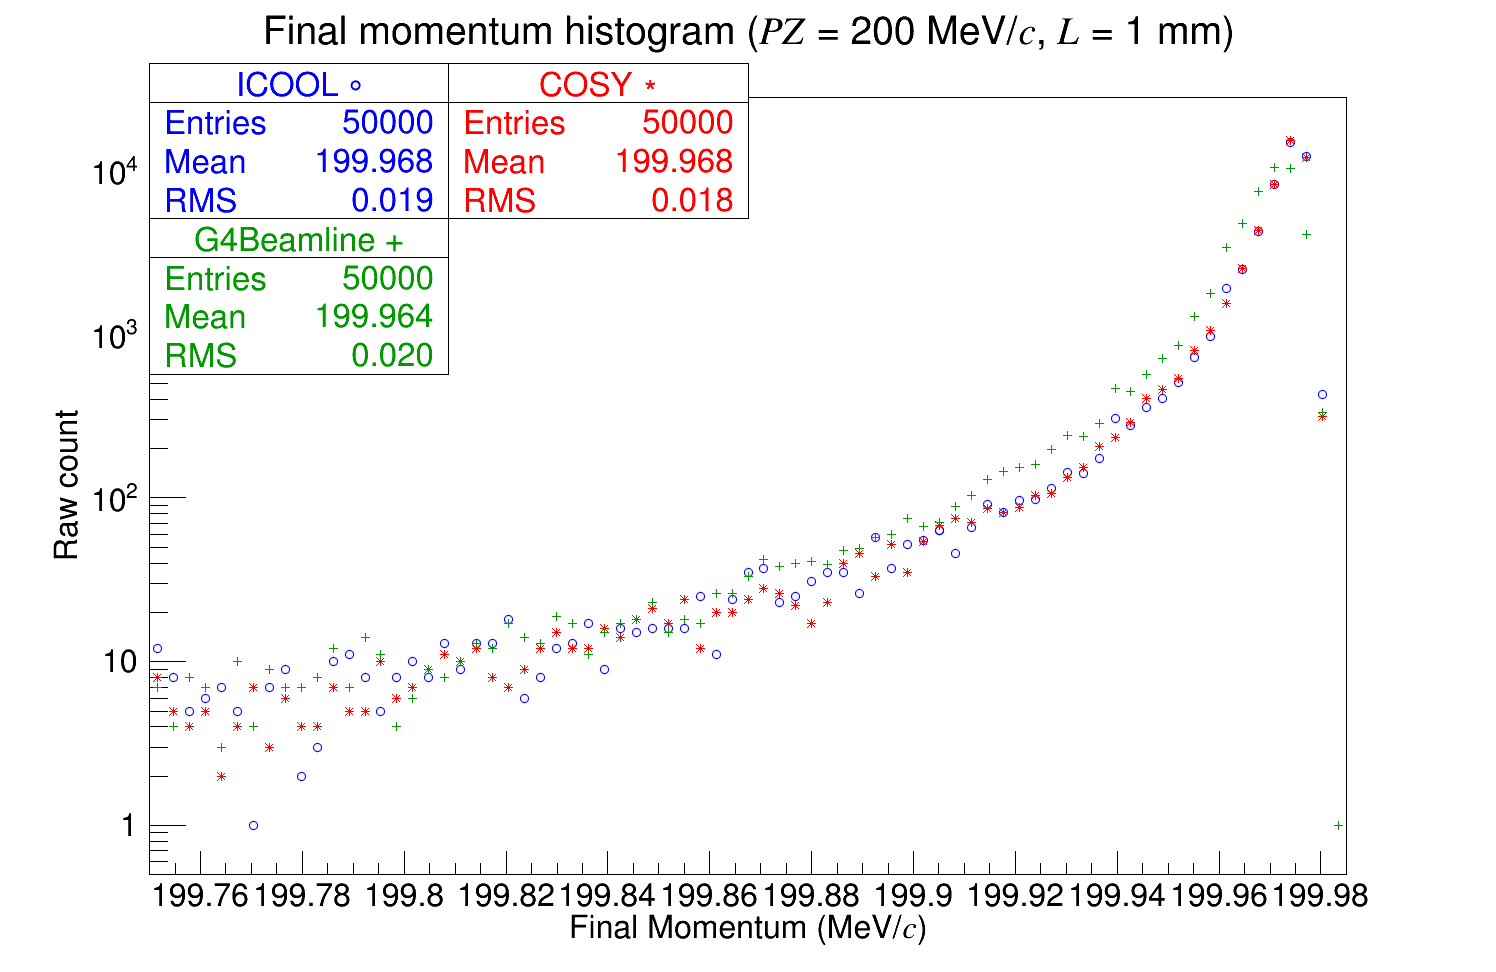
\includegraphics[width=0.7\textwidth]{Benchmarking/LH/strag.200.1.png} 
  \caption[Muons of momentum 100 MeV/$c$ through 1 mm liquid hydrogen.]{Muons of momentum 100 MeV/$c$ through 1 mm liquid hydrogen. Observe that for the $x$ and $p_x$ histograms, COSY and G4Beamline follow a Gaussian-like peak whereas ICOOL follows a Fano peak.}
  \label{fig:200.1}
\end{figure}

\begin{figure}[H]
  \centering
    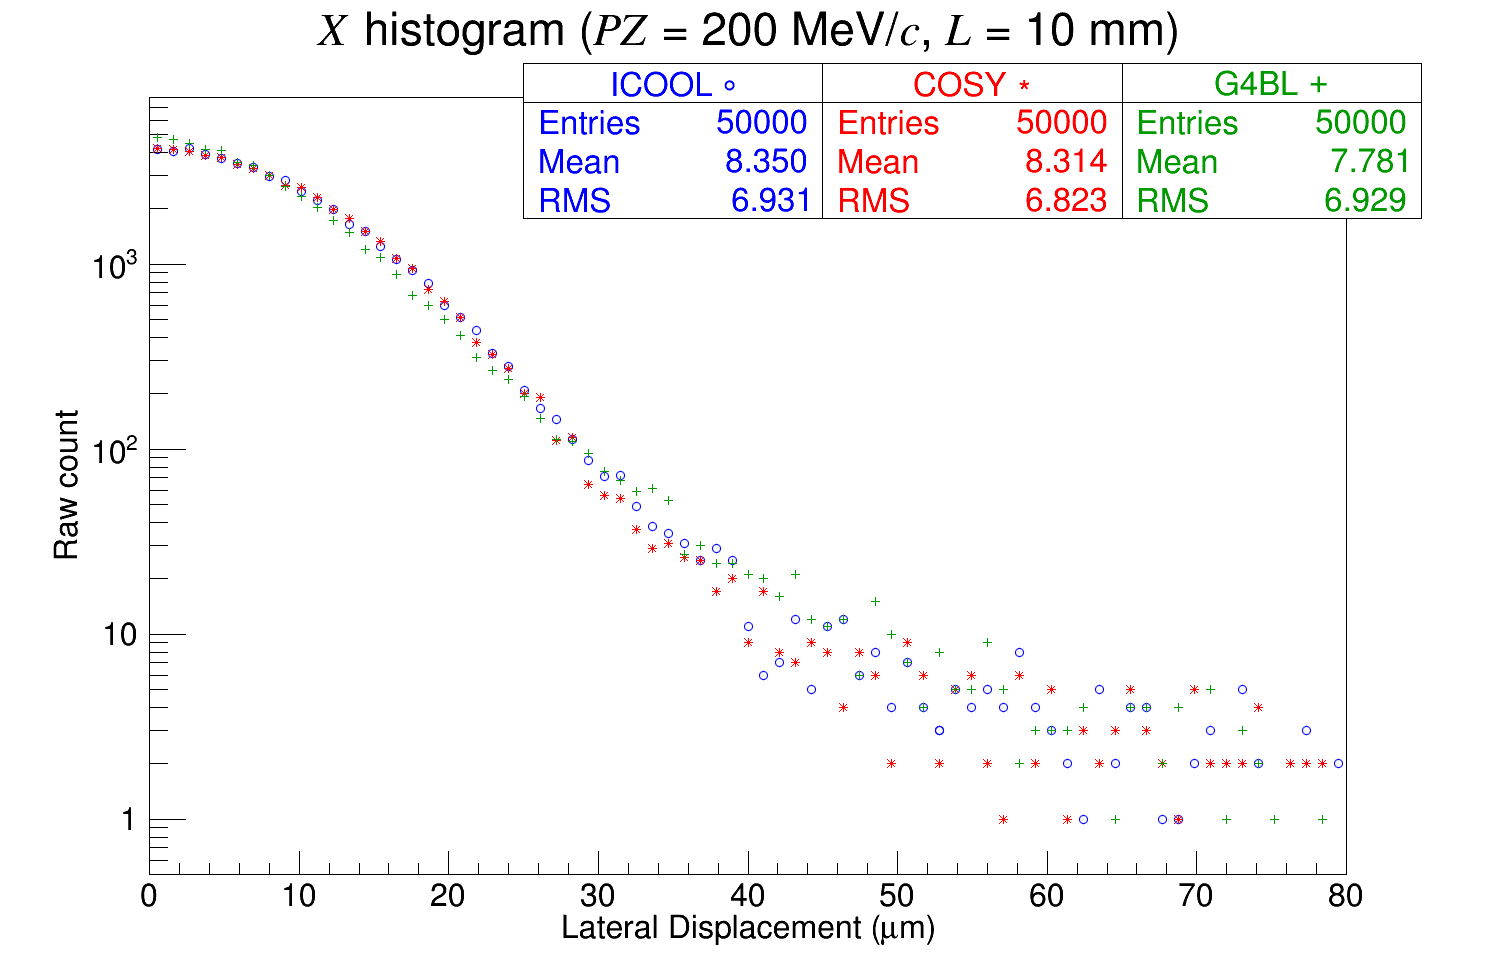
\includegraphics[width=0.7\textwidth]{Benchmarking/LH/X.200.10.png} 
    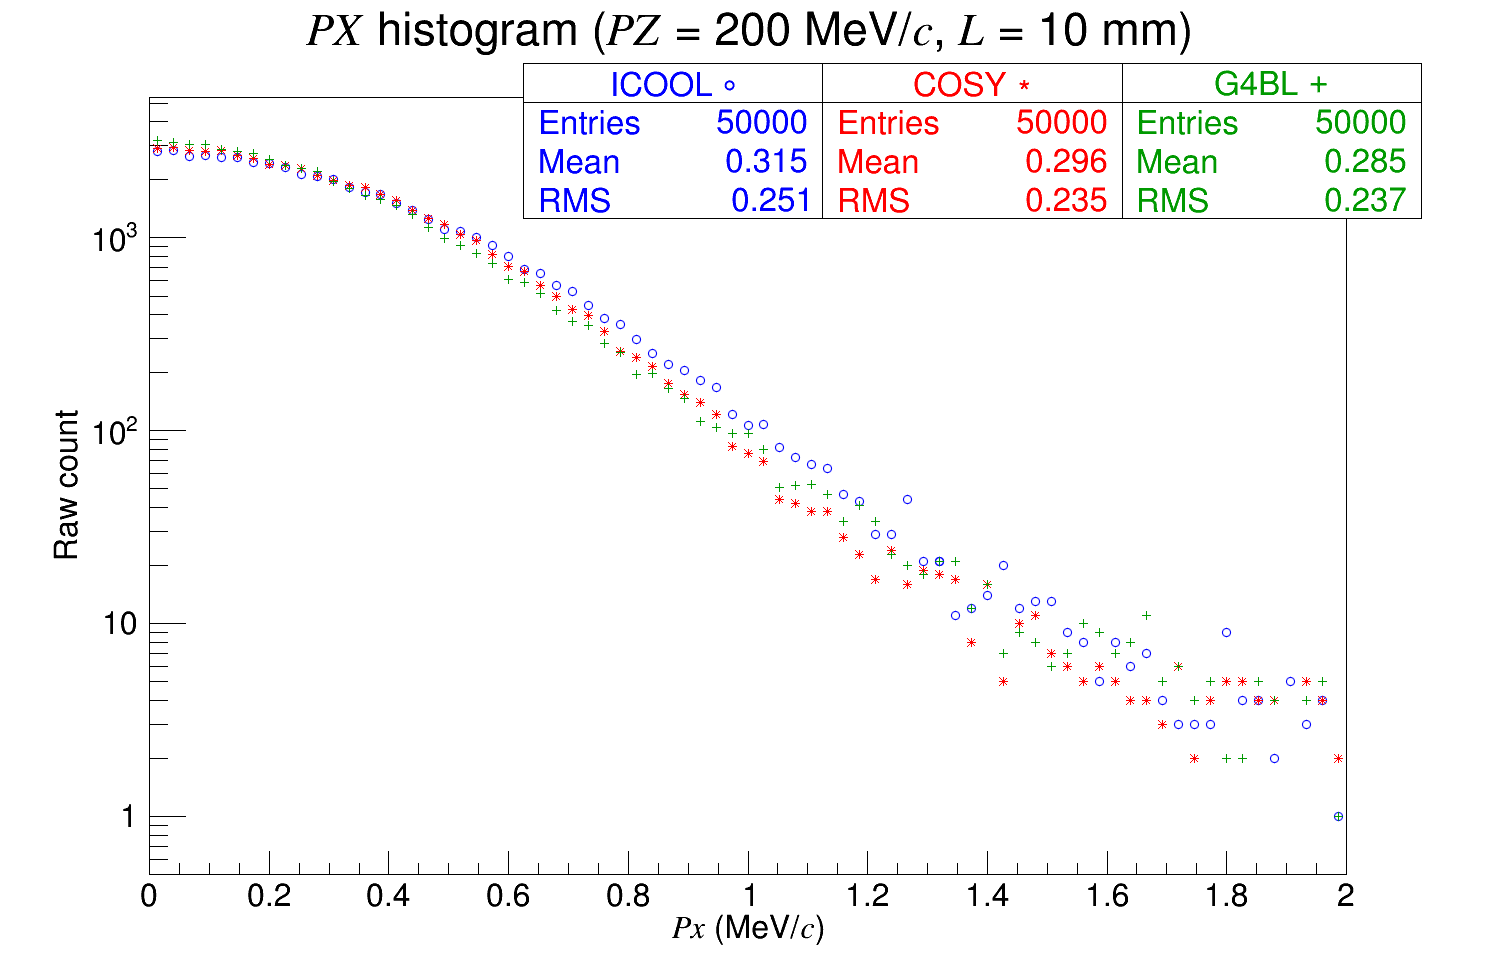
\includegraphics[width=0.7\textwidth]{Benchmarking/LH/PX.200.10.png} 
    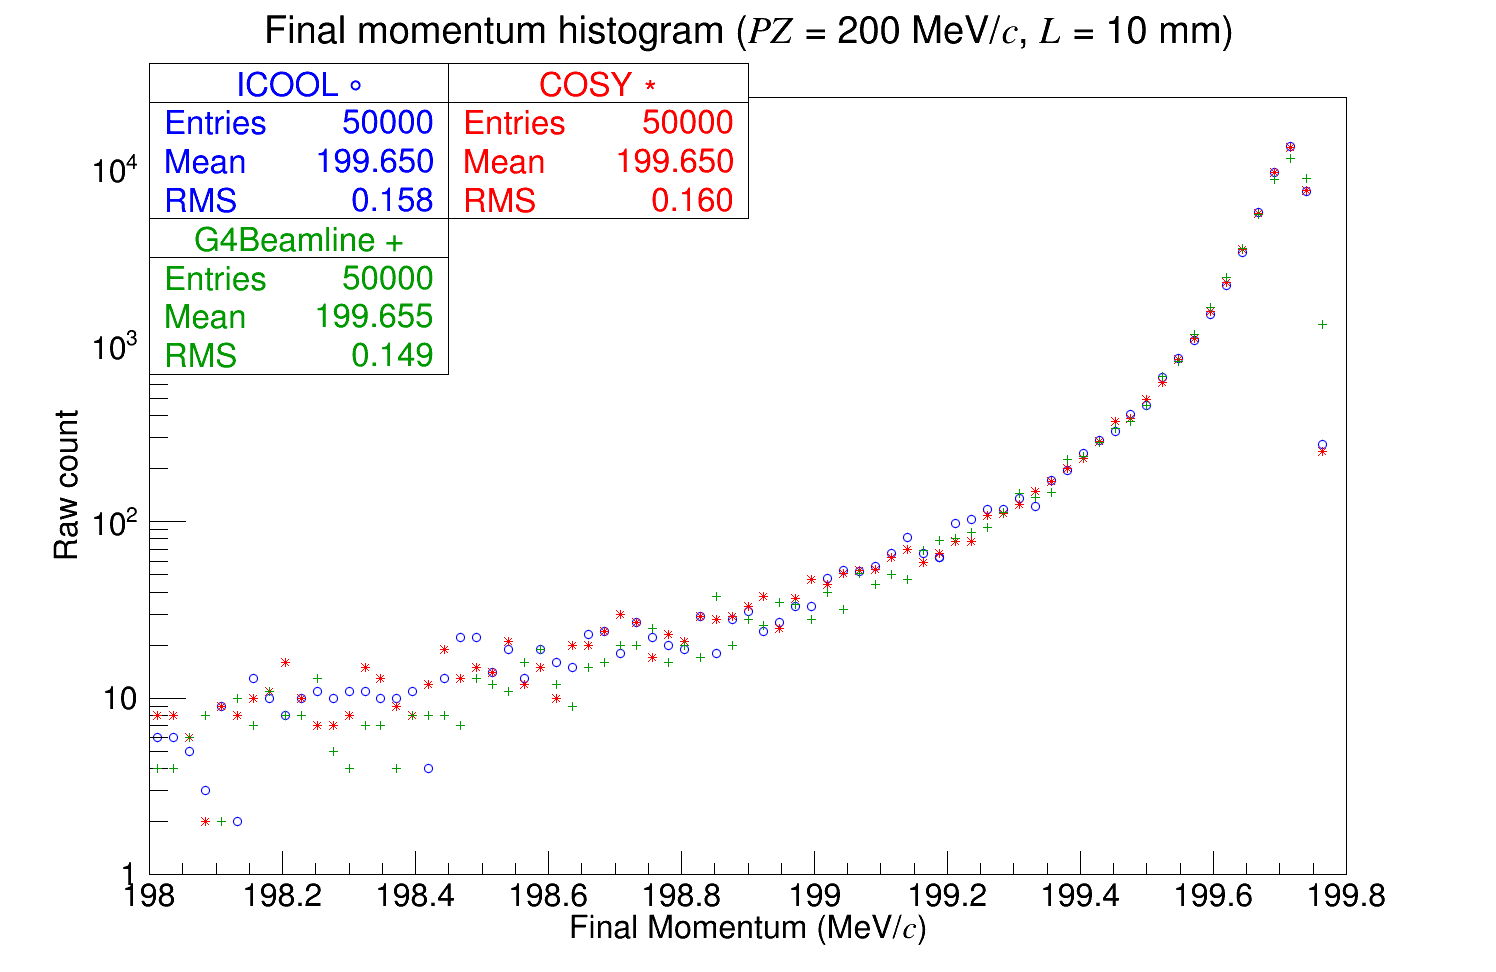
\includegraphics[width=0.7\textwidth]{Benchmarking/LH/strag.200.10.png} 
  \caption{Muons of momentum 200 MeV/$c$ through 10 mm liquid hydrogen.}
  \label{fig:200.10}
\end{figure}

\begin{figure}[H]
  \centering
    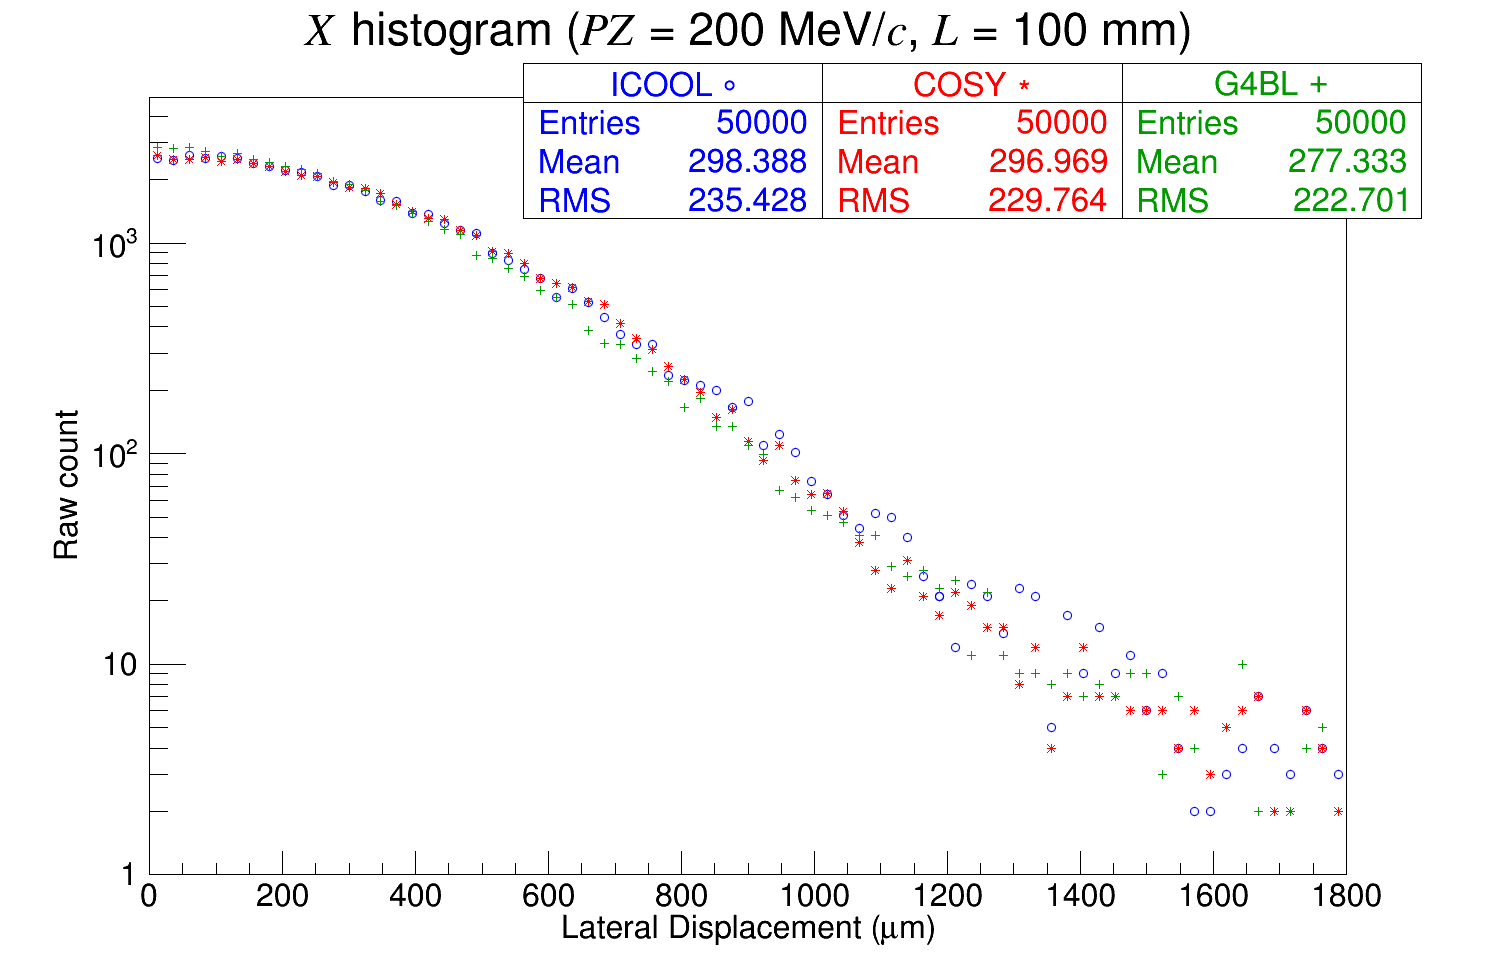
\includegraphics[width=0.7\textwidth]{Benchmarking/LH/X.200.100.png} 
    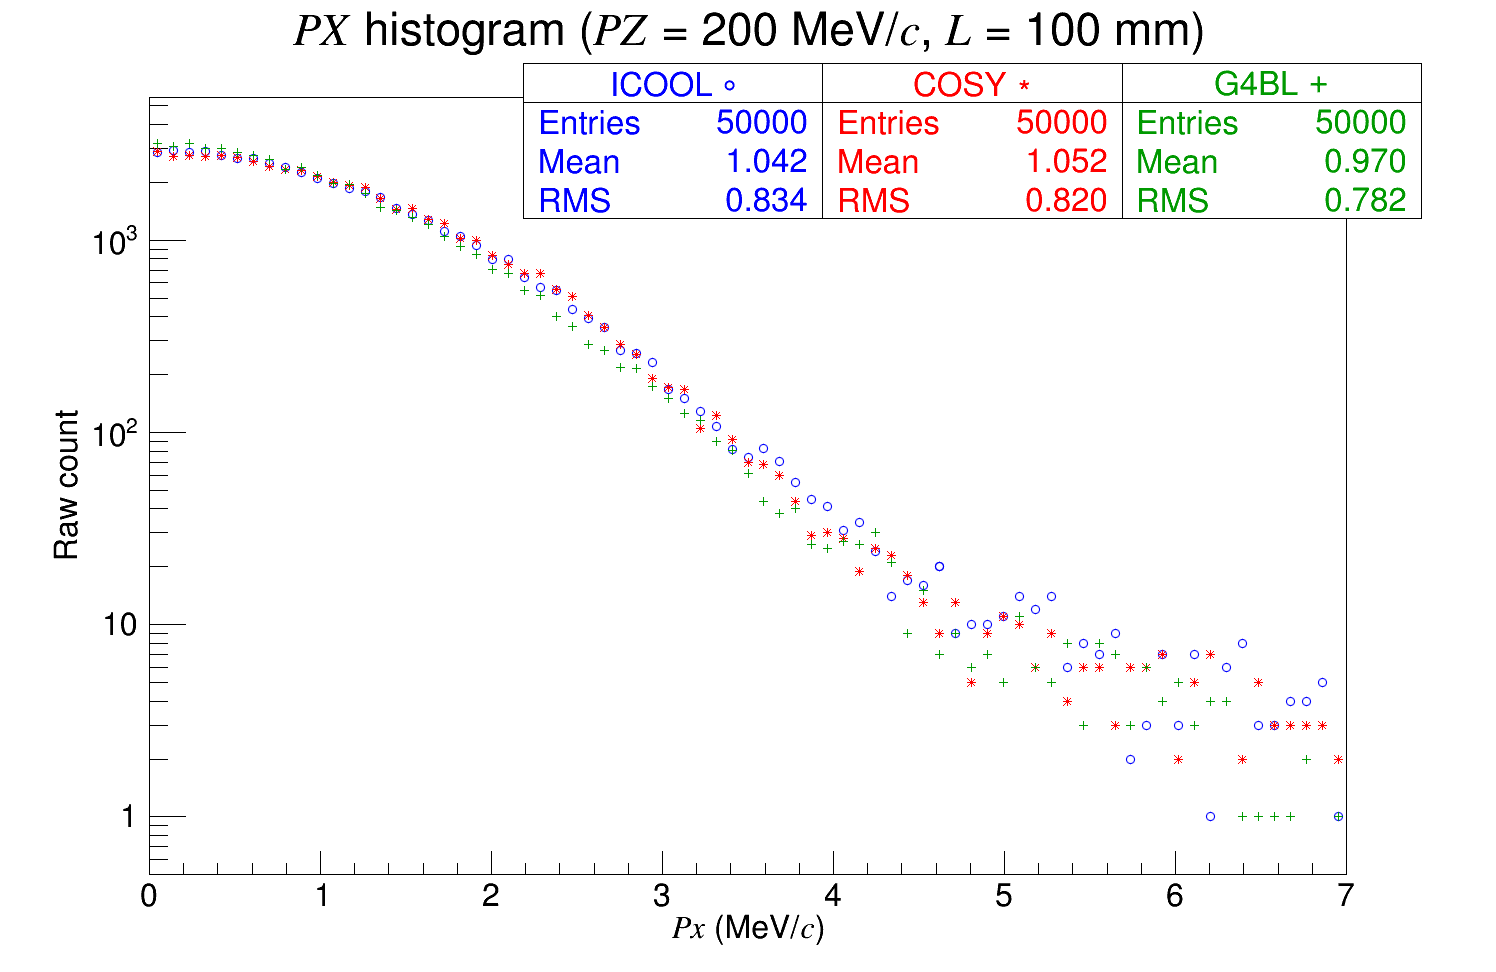
\includegraphics[width=0.7\textwidth]{Benchmarking/LH/PX.200.100.png} 
    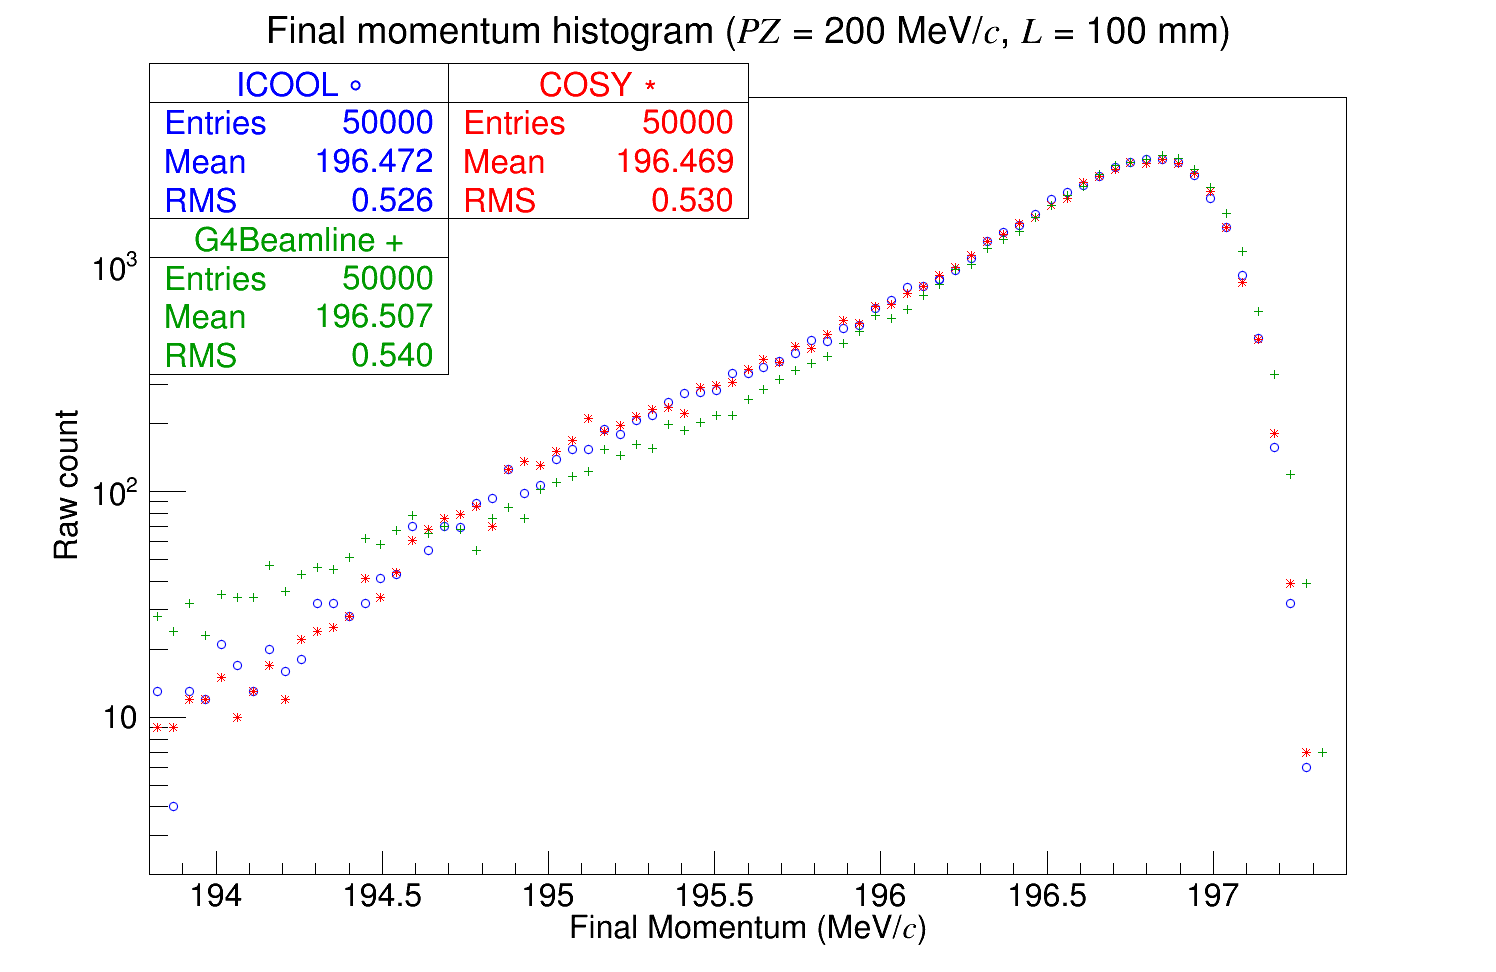
\includegraphics[width=0.7\textwidth]{Benchmarking/LH/strag.200.100.png} 
  \caption{Muons of momentum 200 MeV/$c$ through 100 mm liquid hydrogen.}
  \label{fig:200.100}
\end{figure}

\begin{figure}[H]
  \centering
    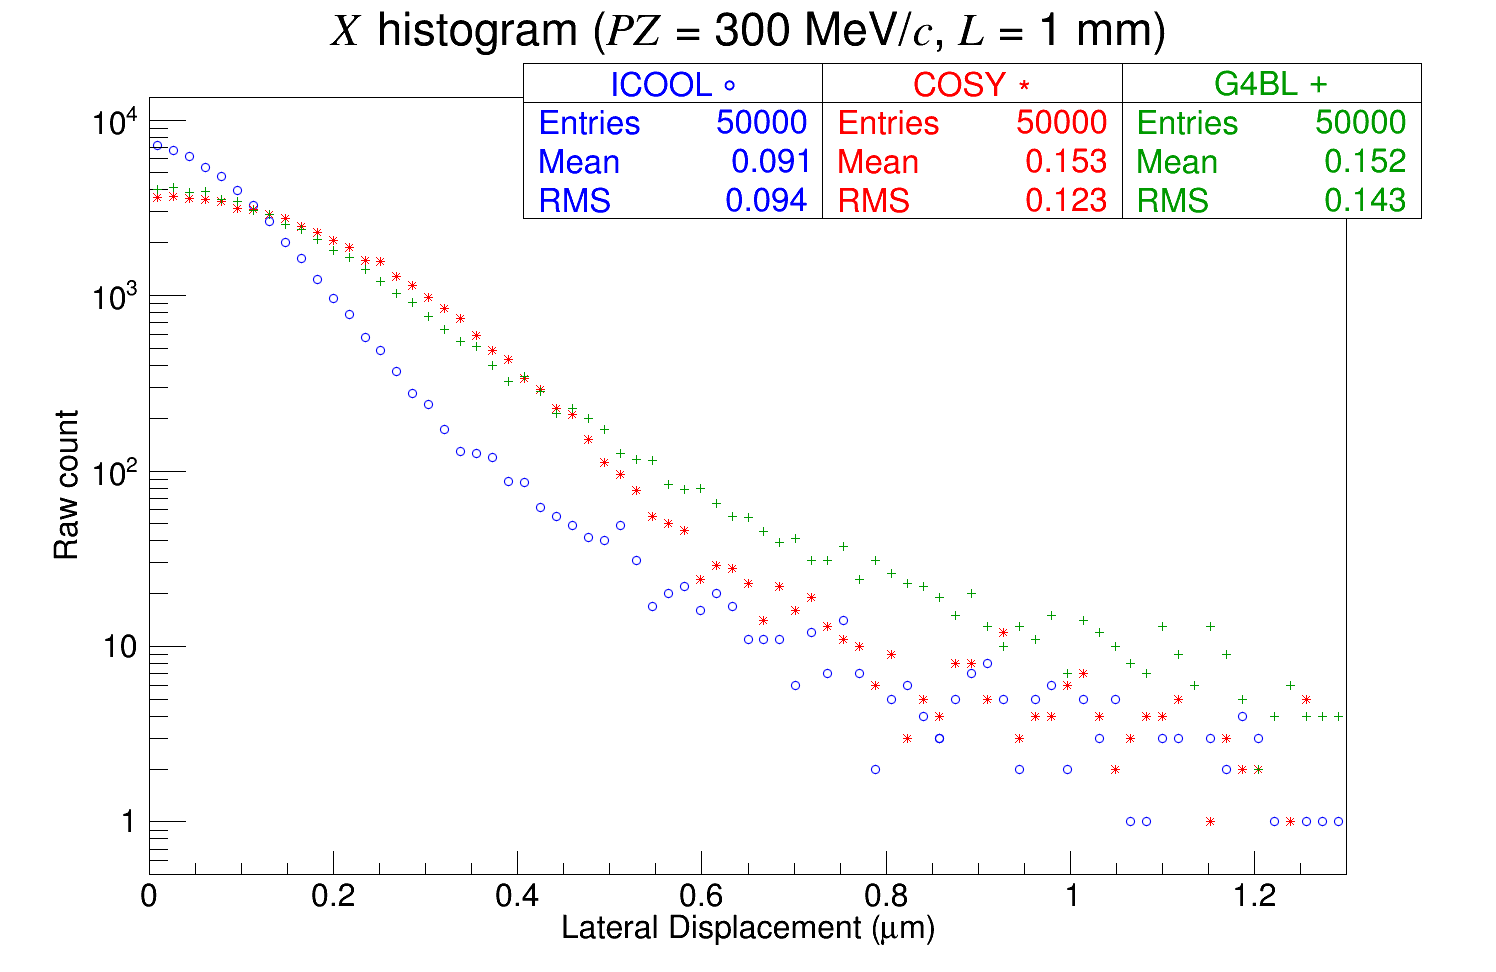
\includegraphics[width=0.7\textwidth]{Benchmarking/LH/X.300.1.png} 
    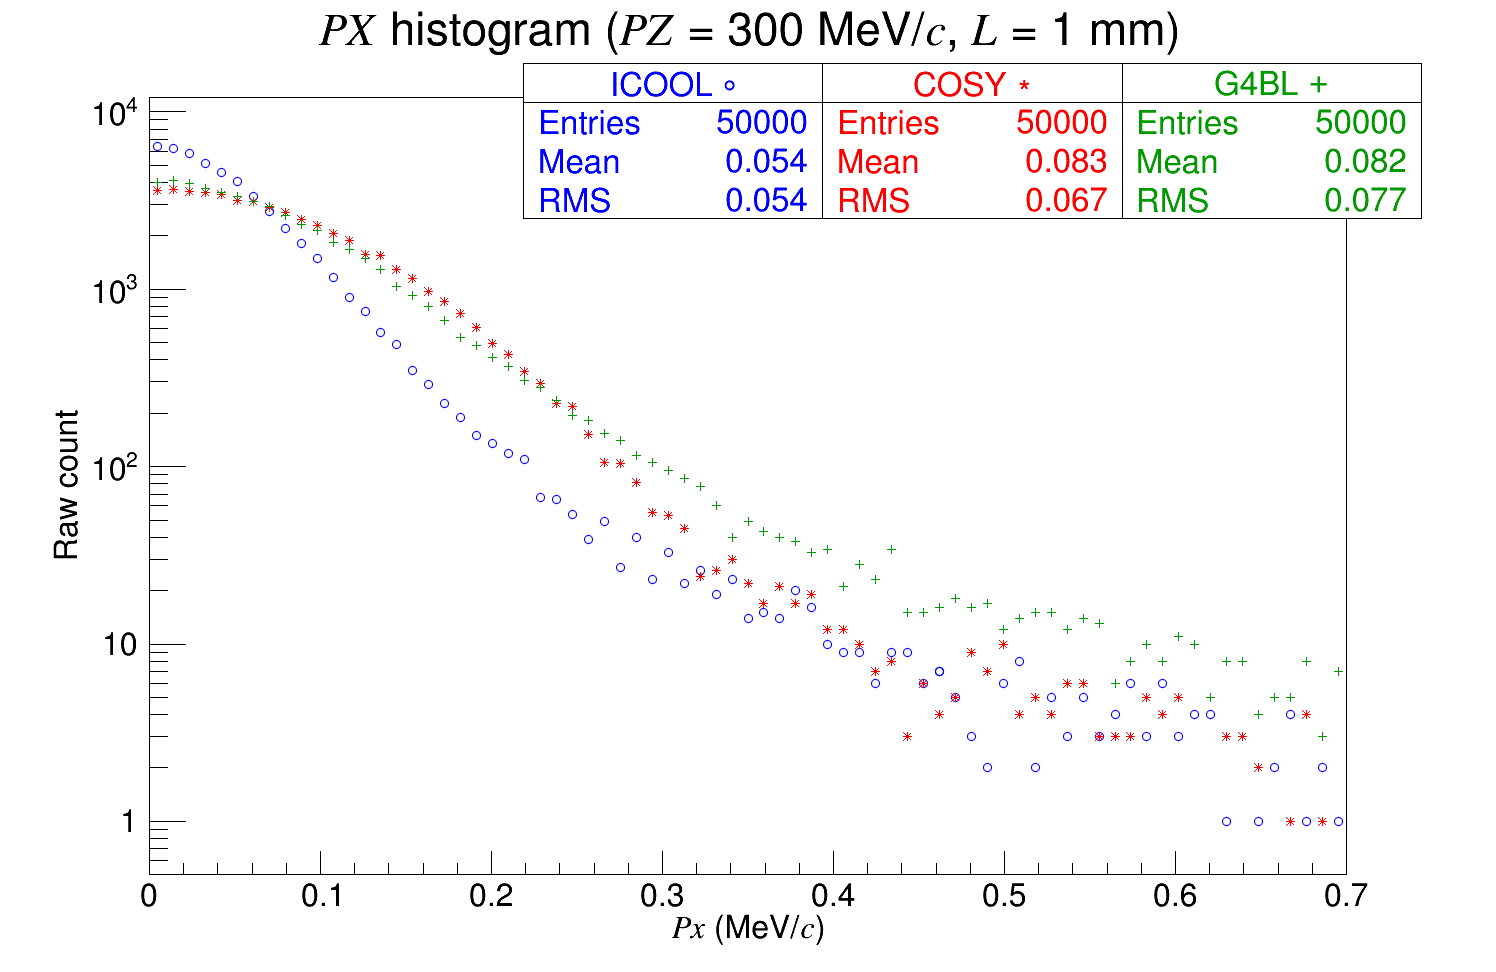
\includegraphics[width=0.7\textwidth]{Benchmarking/LH/PX.300.1.png} 
    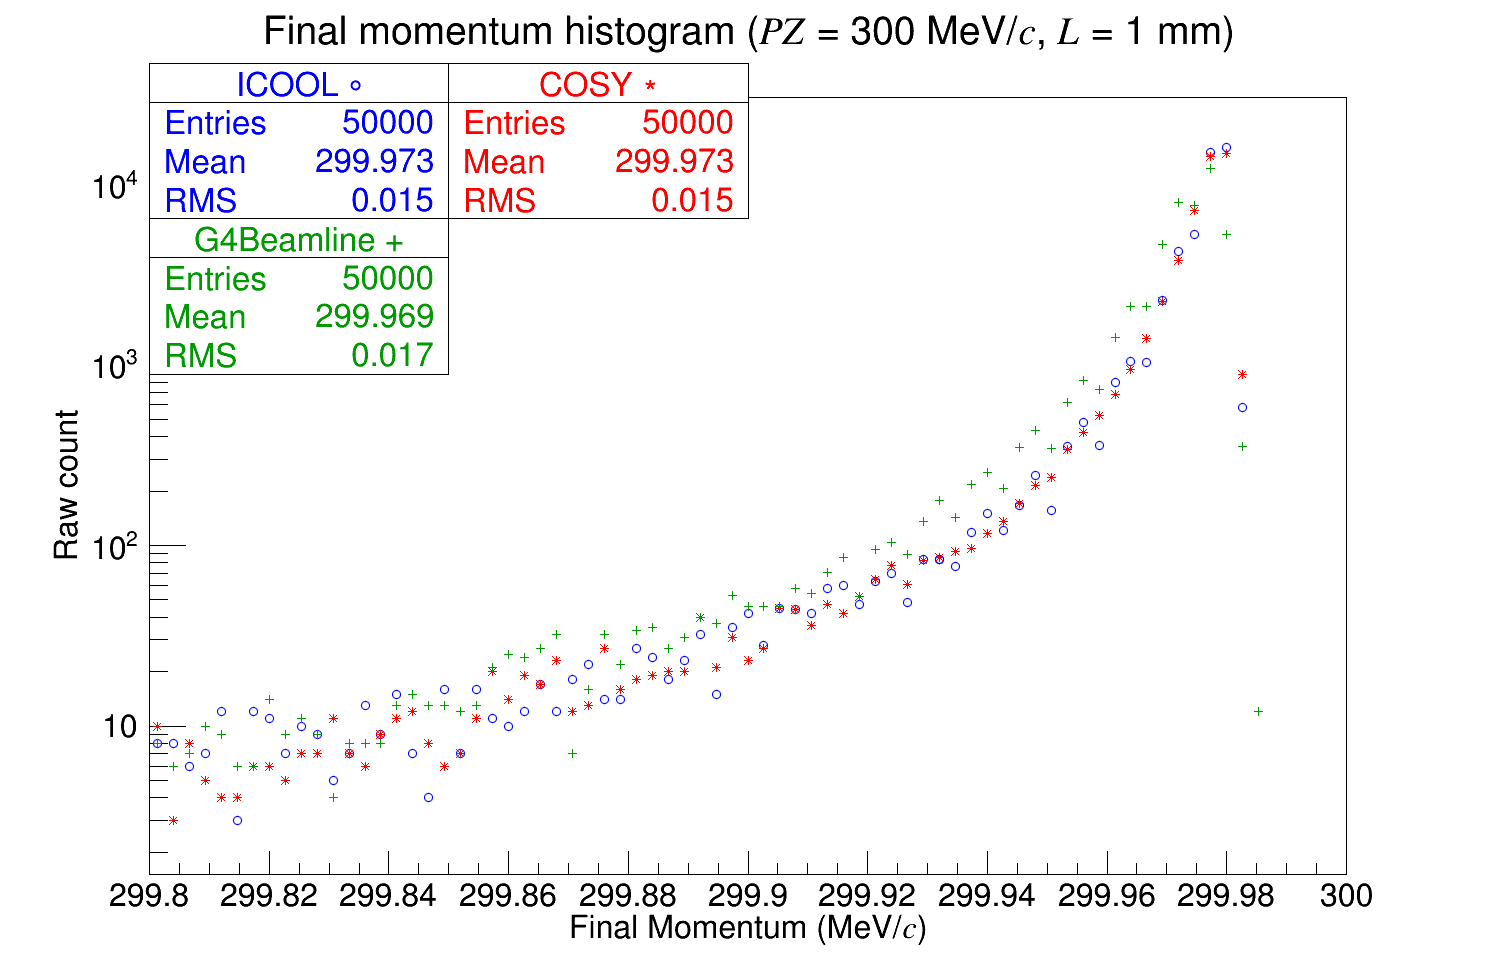
\includegraphics[width=0.7\textwidth]{Benchmarking/LH/strag.300.1.png} 
  \caption[Muons of momentum 100 MeV/$c$ through 1 mm liquid hydrogen.]{Muons of momentum 100 MeV/$c$ through 1 mm liquid hydrogen. Observe that for the $x$ and $p_x$ histograms, COSY and G4Beamline follow a Gaussian-like peak whereas ICOOL follows a Fano peak.}
  \label{fig:300.1}
\end{figure}


\begin{figure}[H]
  \centering
    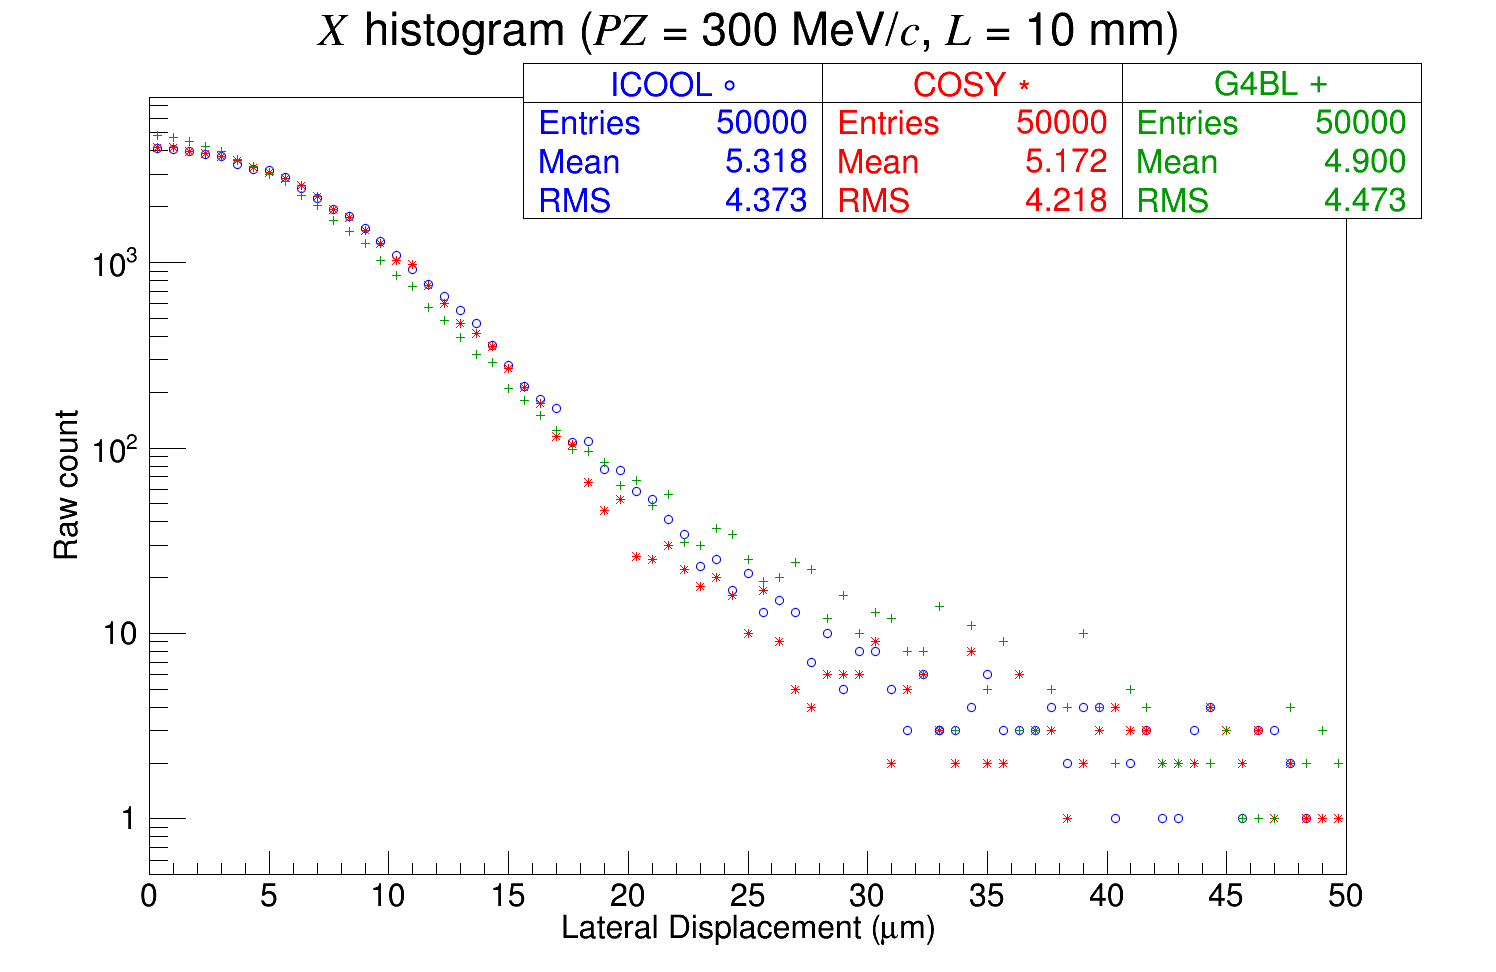
\includegraphics[width=0.7\textwidth]{Benchmarking/LH/X.300.10.png} 
    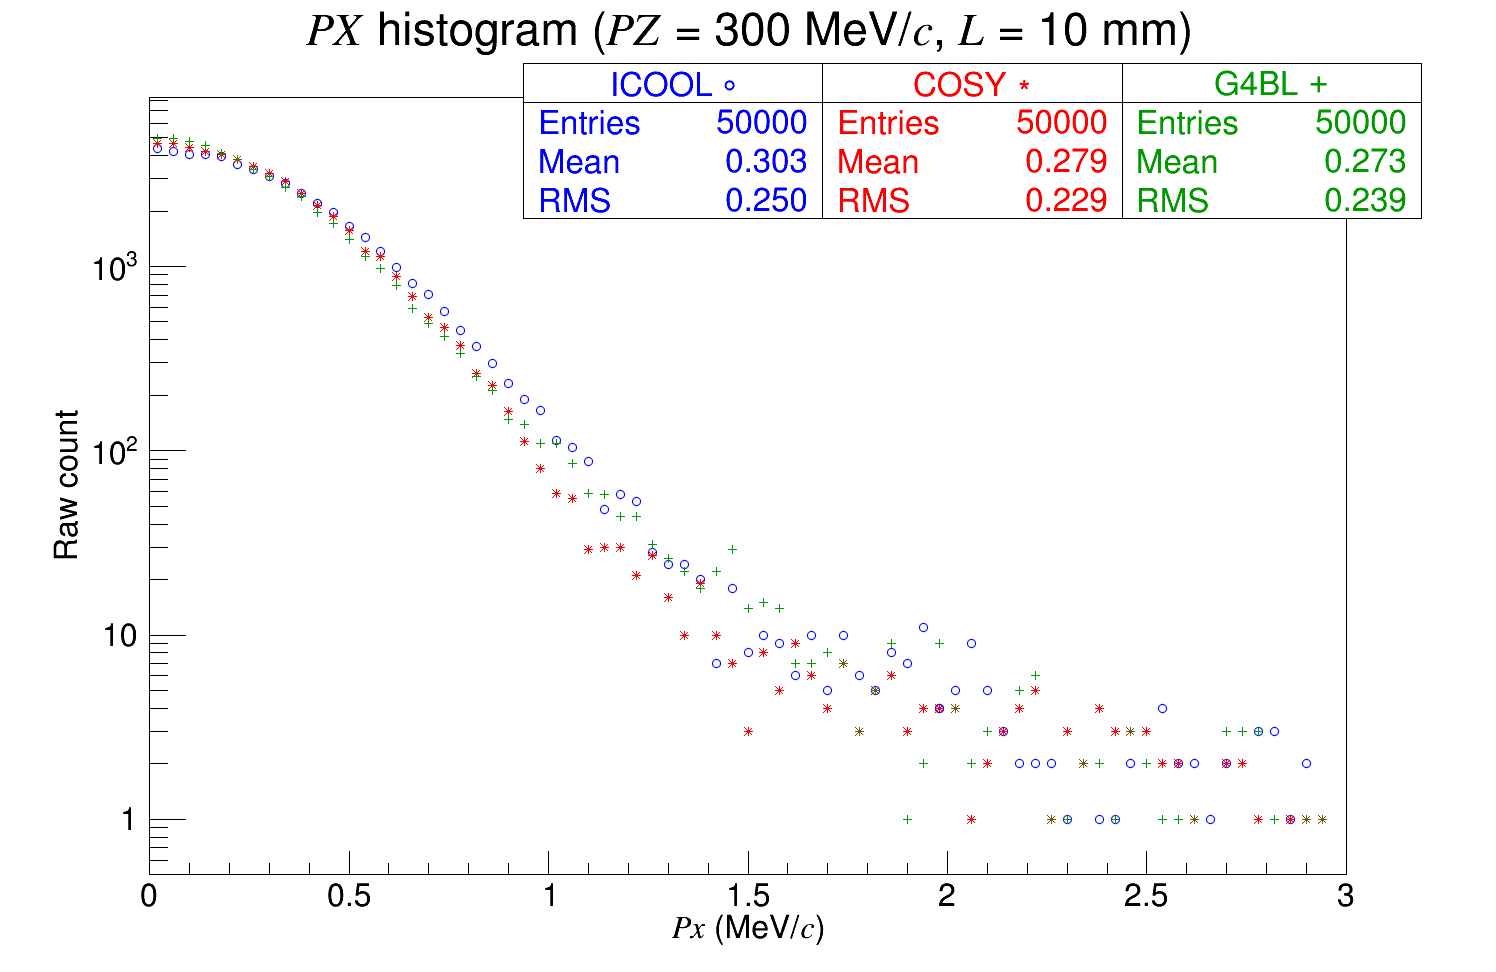
\includegraphics[width=0.7\textwidth]{Benchmarking/LH/PX.300.10.png} 
    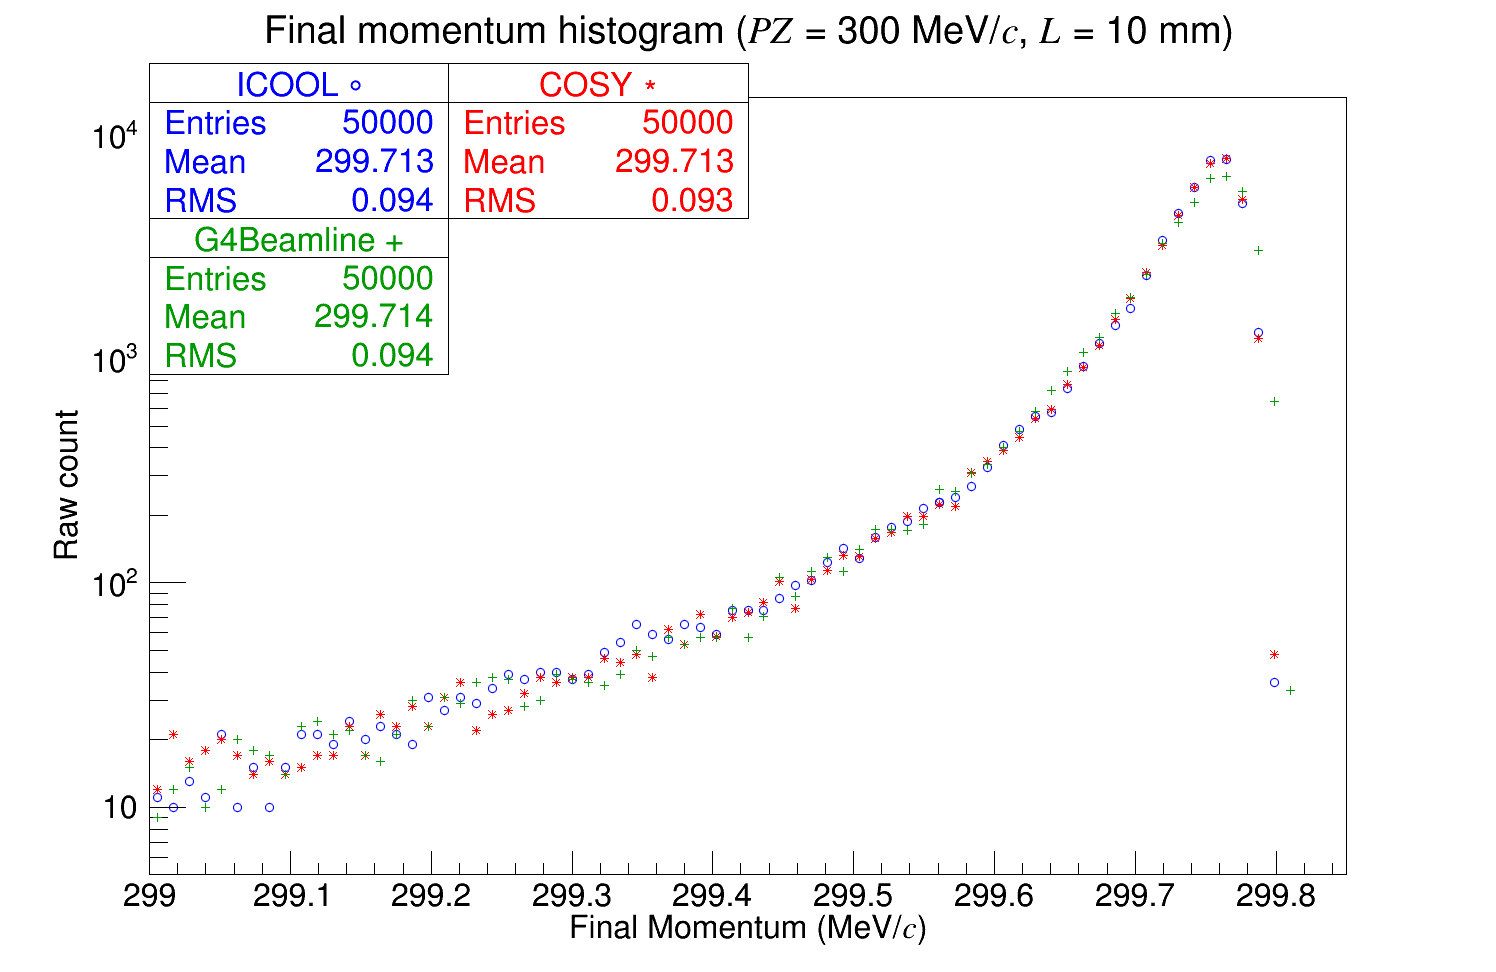
\includegraphics[width=0.7\textwidth]{Benchmarking/LH/strag.300.10.png} 
  \caption{Muons of momentum 300 MeV/$c$ through 10 mm liquid hydrogen.}
  \label{fig:300.10}
\end{figure}

\begin{figure}[!htb]
  \centering
    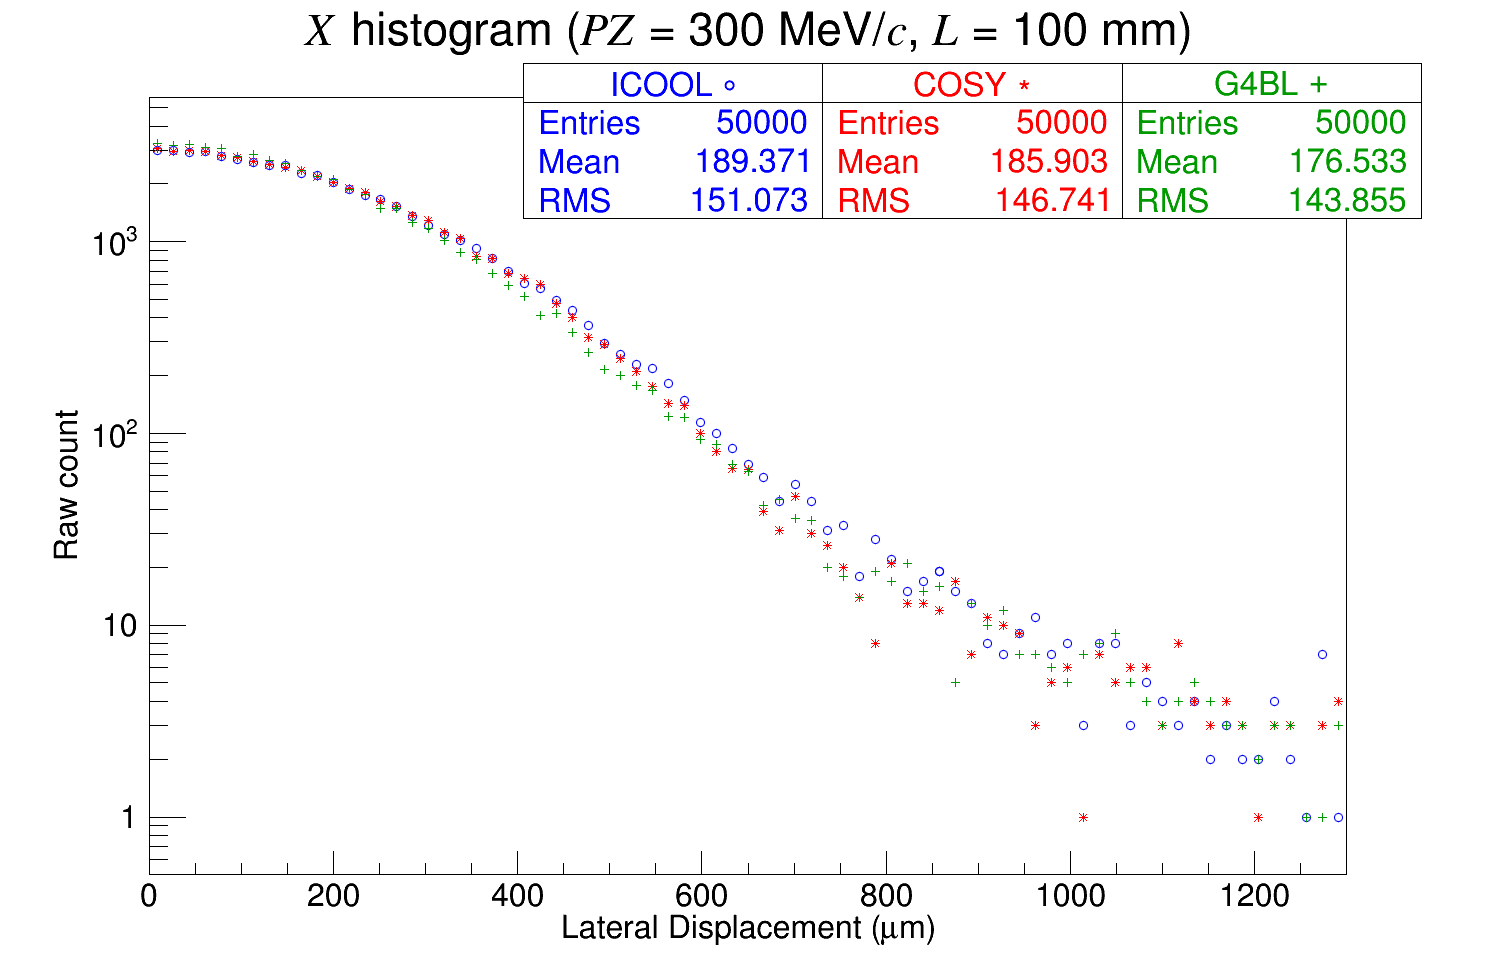
\includegraphics[width=0.7\textwidth]{Benchmarking/LH/X.300.100.png} 
    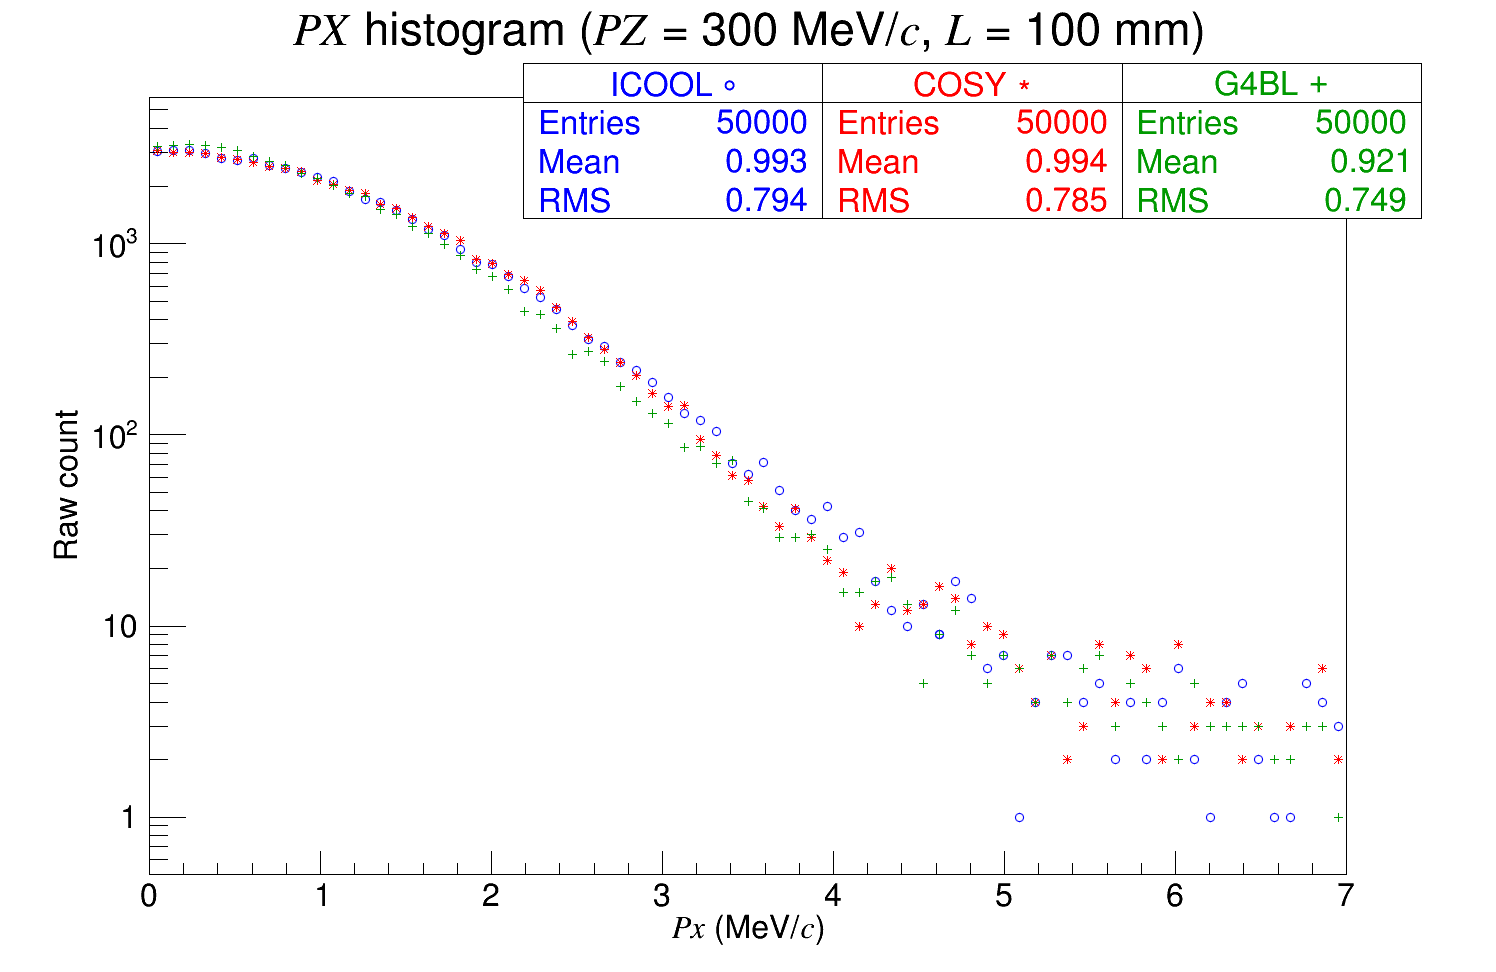
\includegraphics[width=0.7\textwidth]{Benchmarking/LH/PX.300.100.png} 
    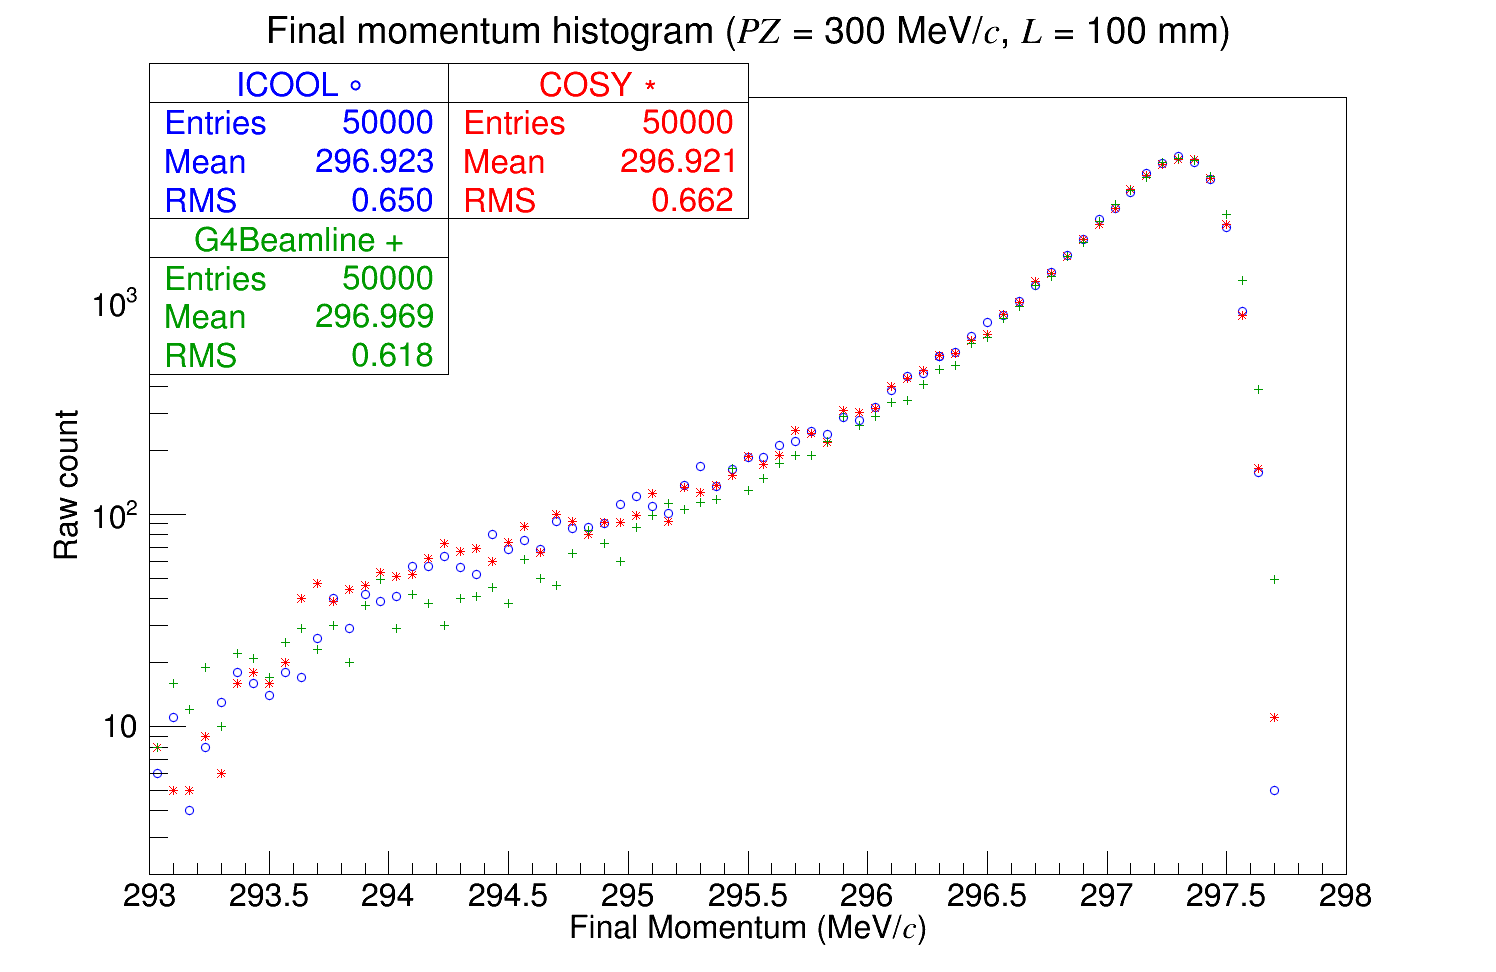
\includegraphics[width=0.7\textwidth]{Benchmarking/LH/strag.300.100.png} 
  \caption{Muons of momentum 300 MeV/$c$ through 100 mm liquid hydrogen.}
  \label{fig:300.100}
\end{figure}

\begin{figure}[H]
  \centering
    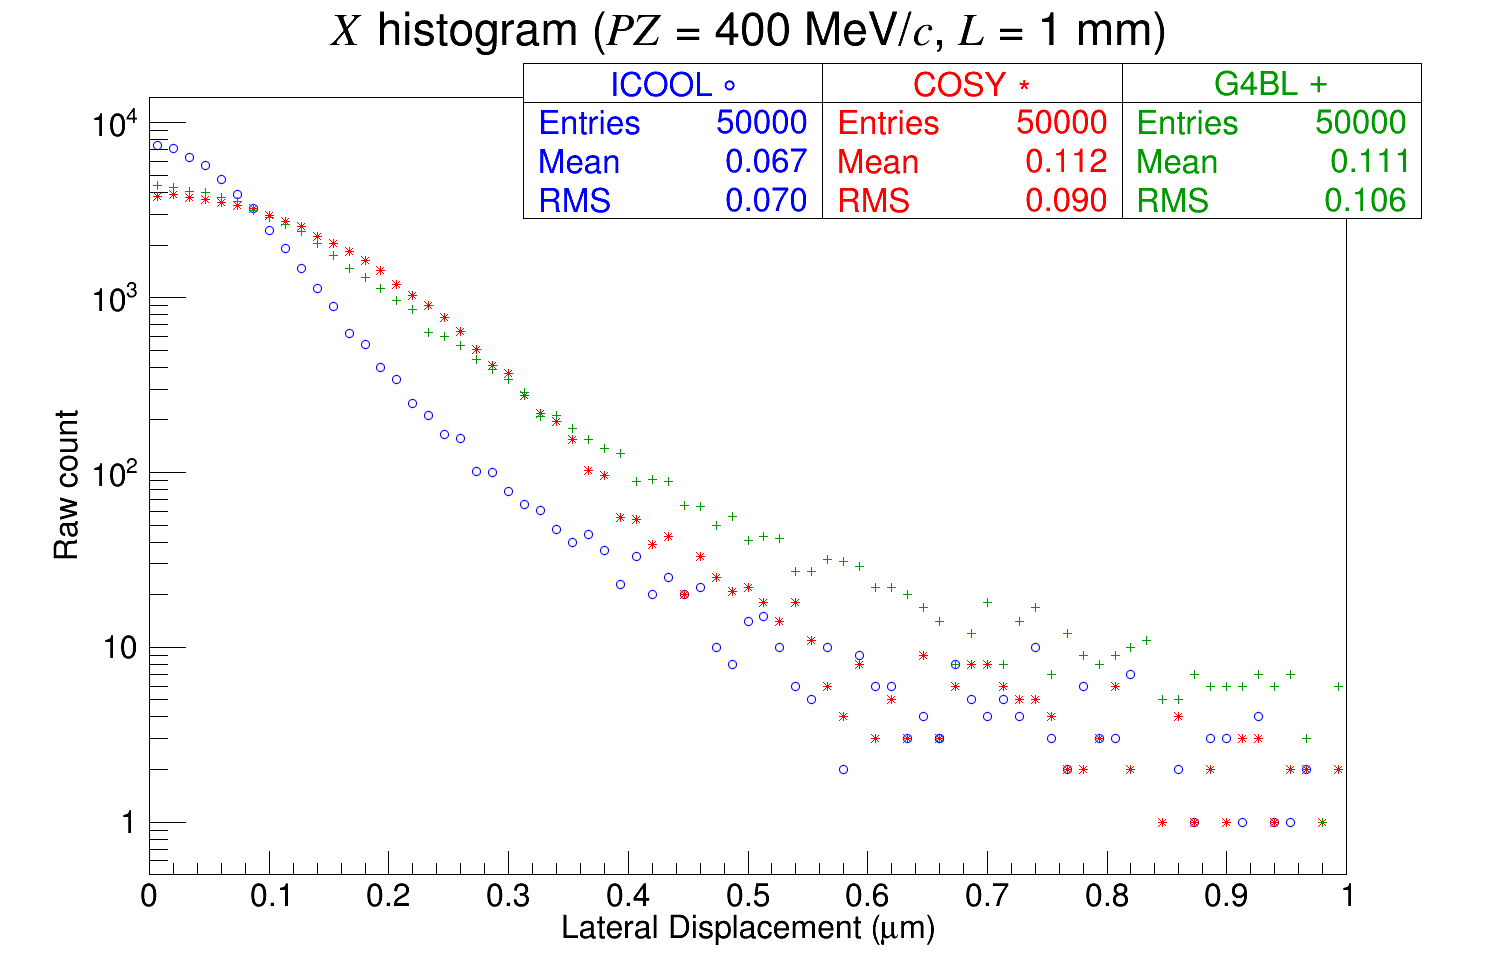
\includegraphics[width=0.7\textwidth]{Benchmarking/LH/X.400.1.png} 
    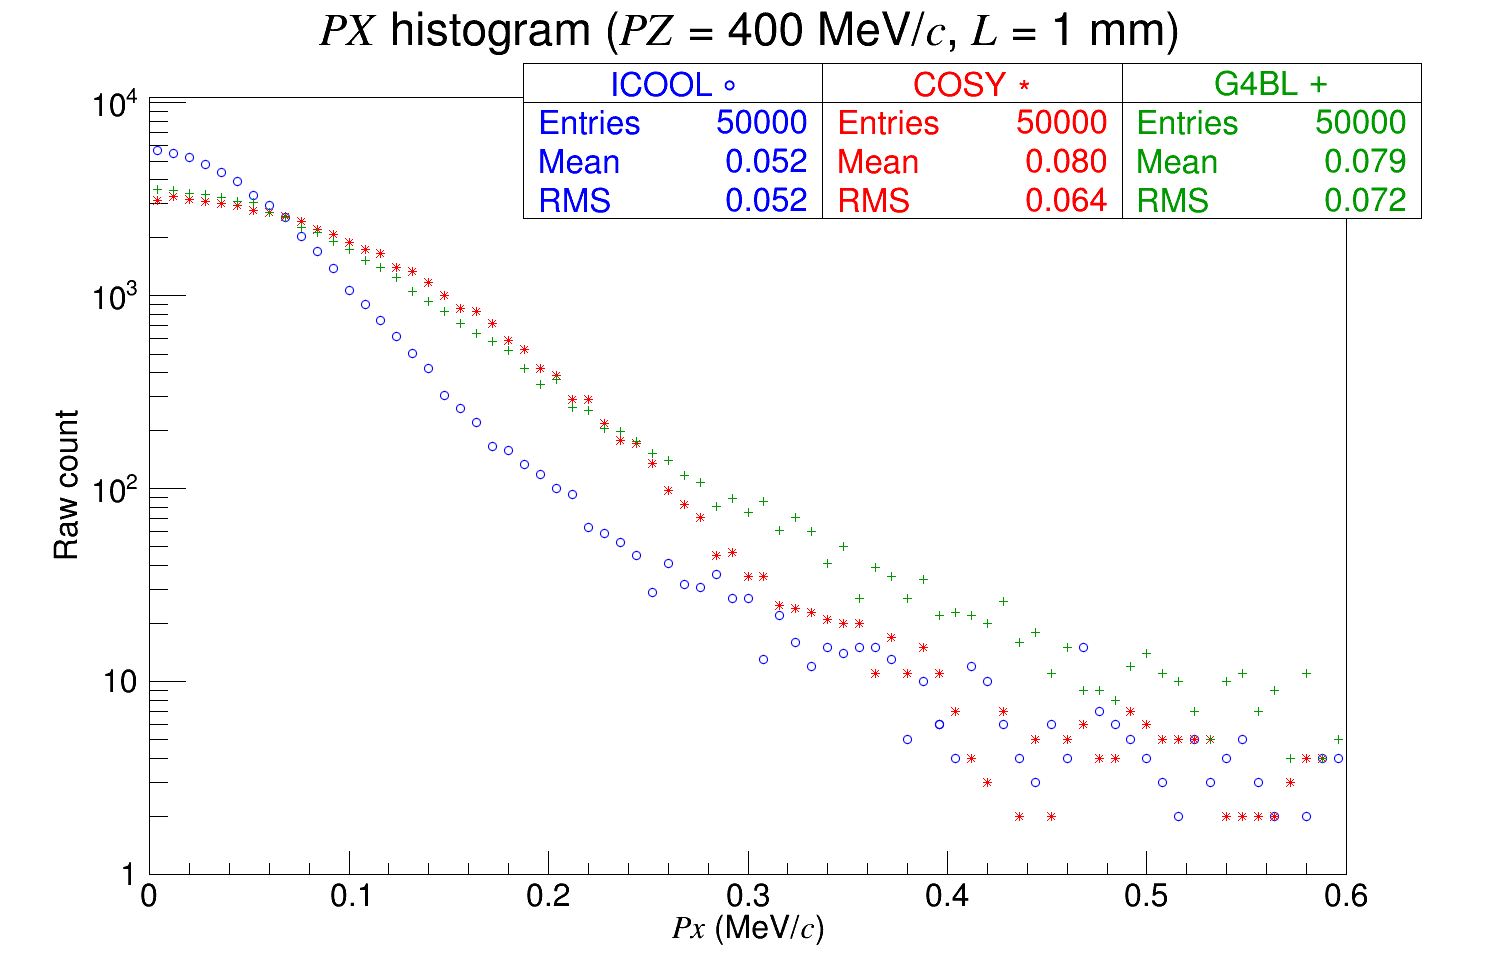
\includegraphics[width=0.7\textwidth]{Benchmarking/LH/PX.400.1.png} 
    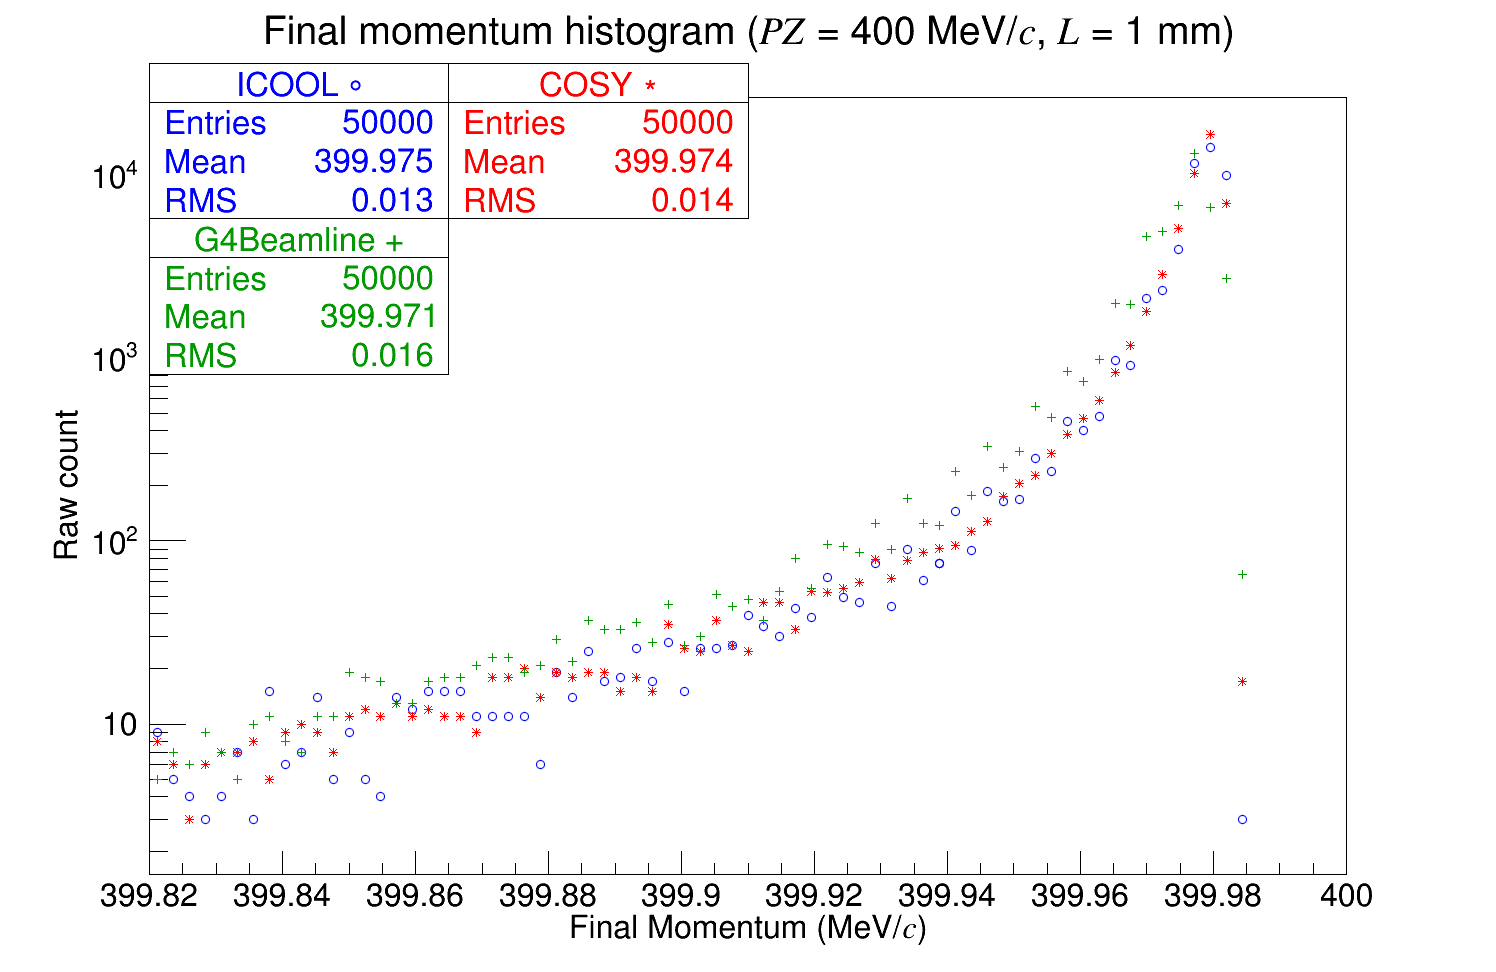
\includegraphics[width=0.7\textwidth]{Benchmarking/LH/strag.400.1.png} 
  \caption[Muons of momentum 100 MeV/$c$ through 1 mm liquid hydrogen.]{Muons of momentum 100 MeV/$c$ through 1 mm liquid hydrogen. Observe that for the $x$ and $p_x$ histograms, COSY and G4Beamline follow a Gaussian-like peak whereas ICOOL follows a Fano peak.}
  \label{fig:400.1}
\end{figure}

\begin{figure}[H]
  \centering
    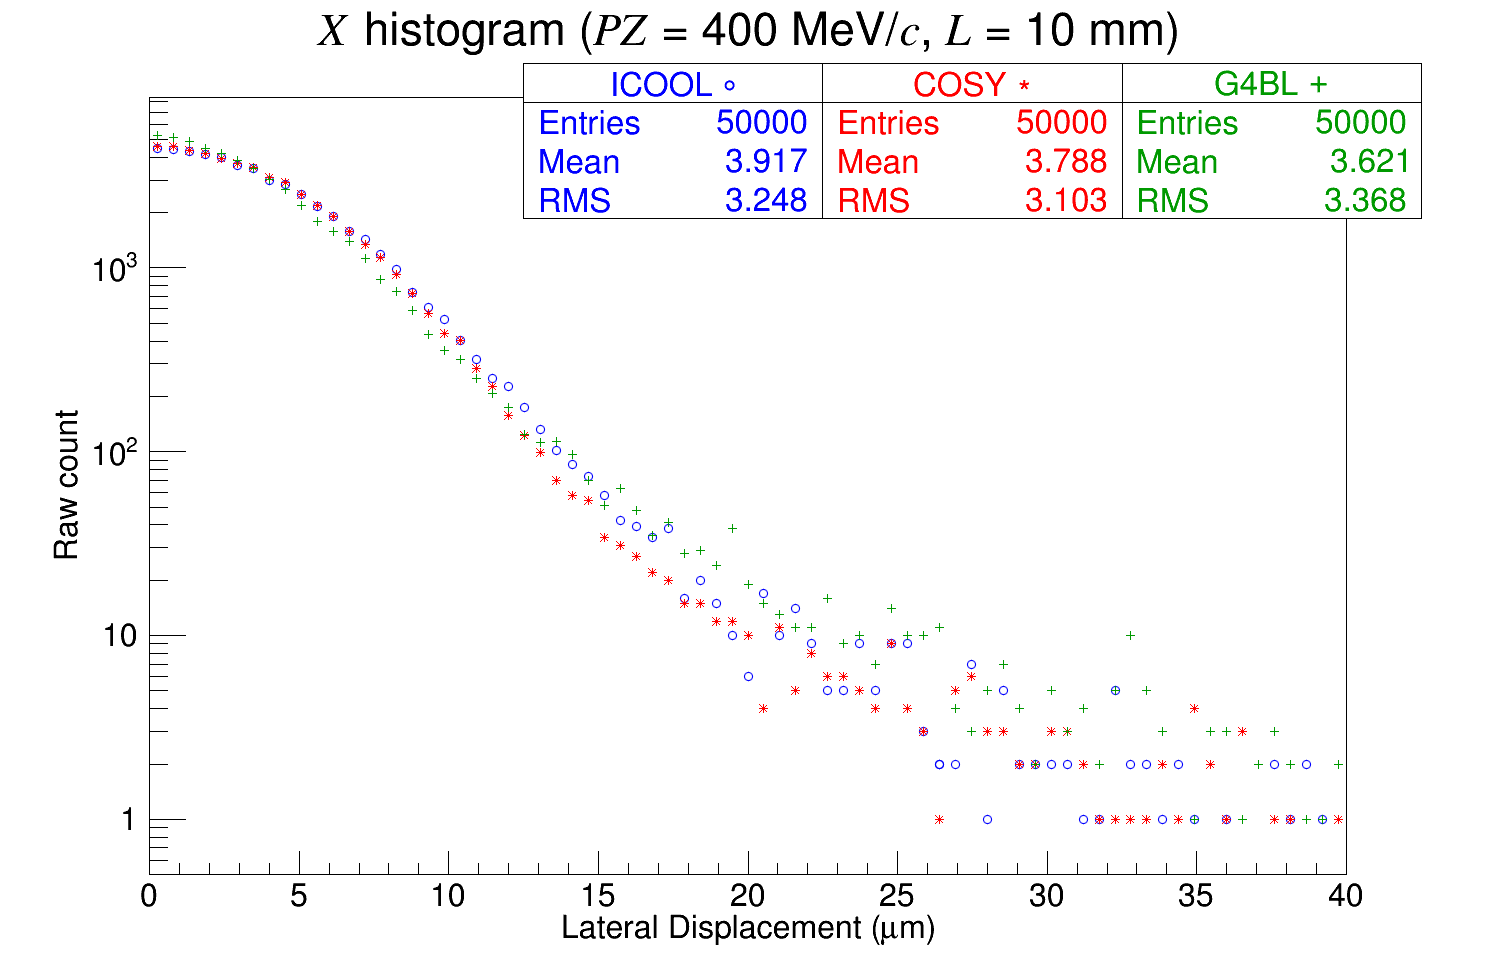
\includegraphics[width=0.7\textwidth]{Benchmarking/LH/X.400.10.png} 
    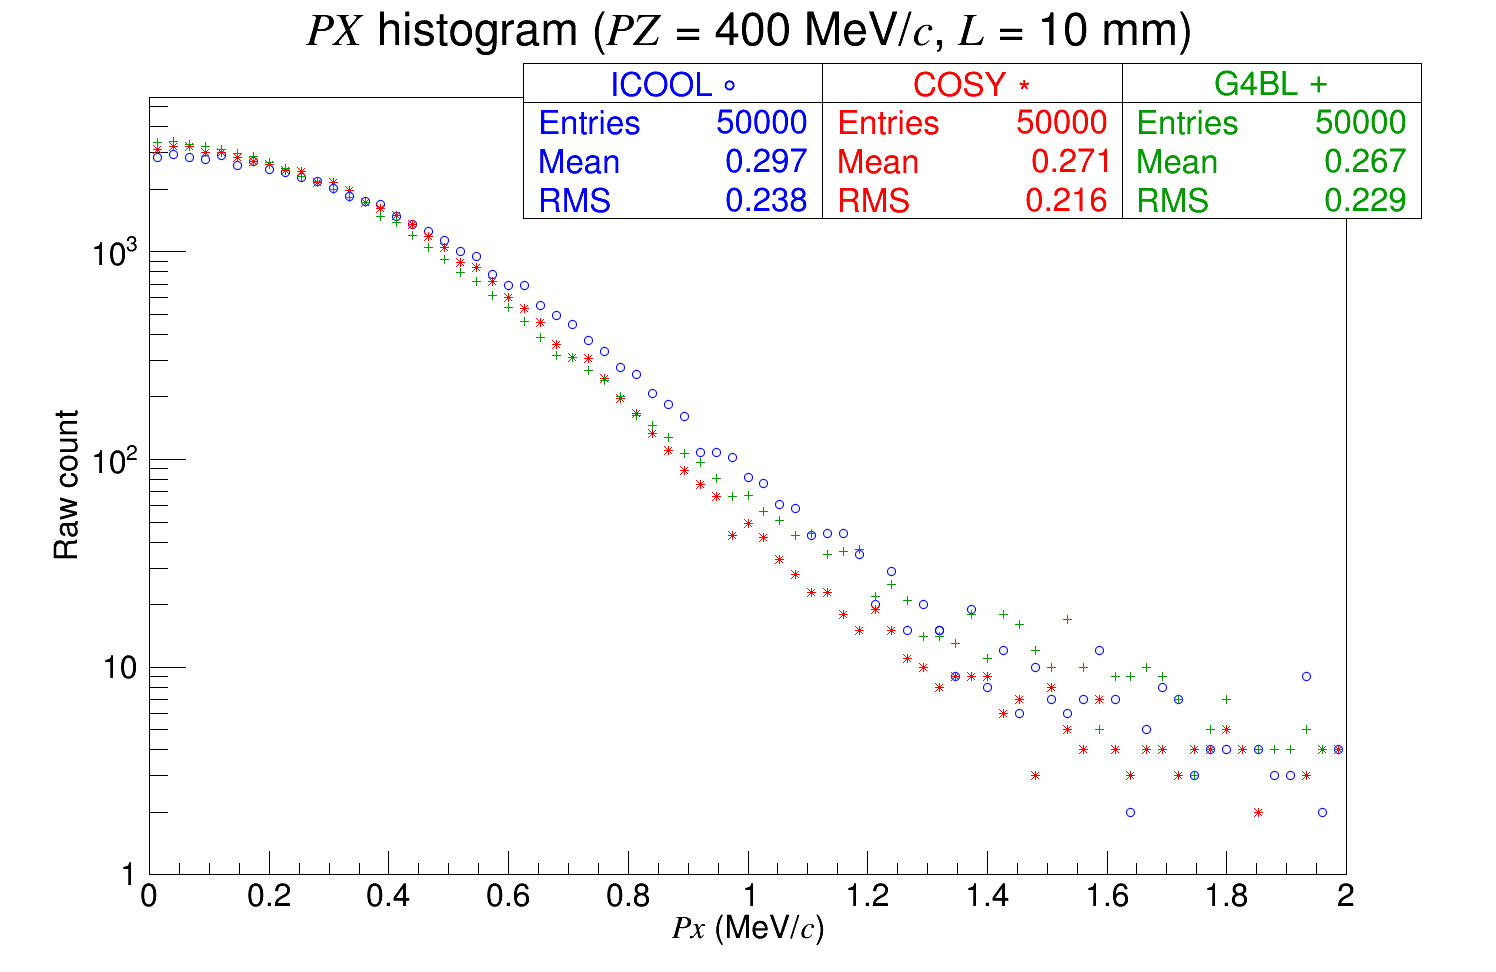
\includegraphics[width=0.7\textwidth]{Benchmarking/LH/PX.400.10.png} 
    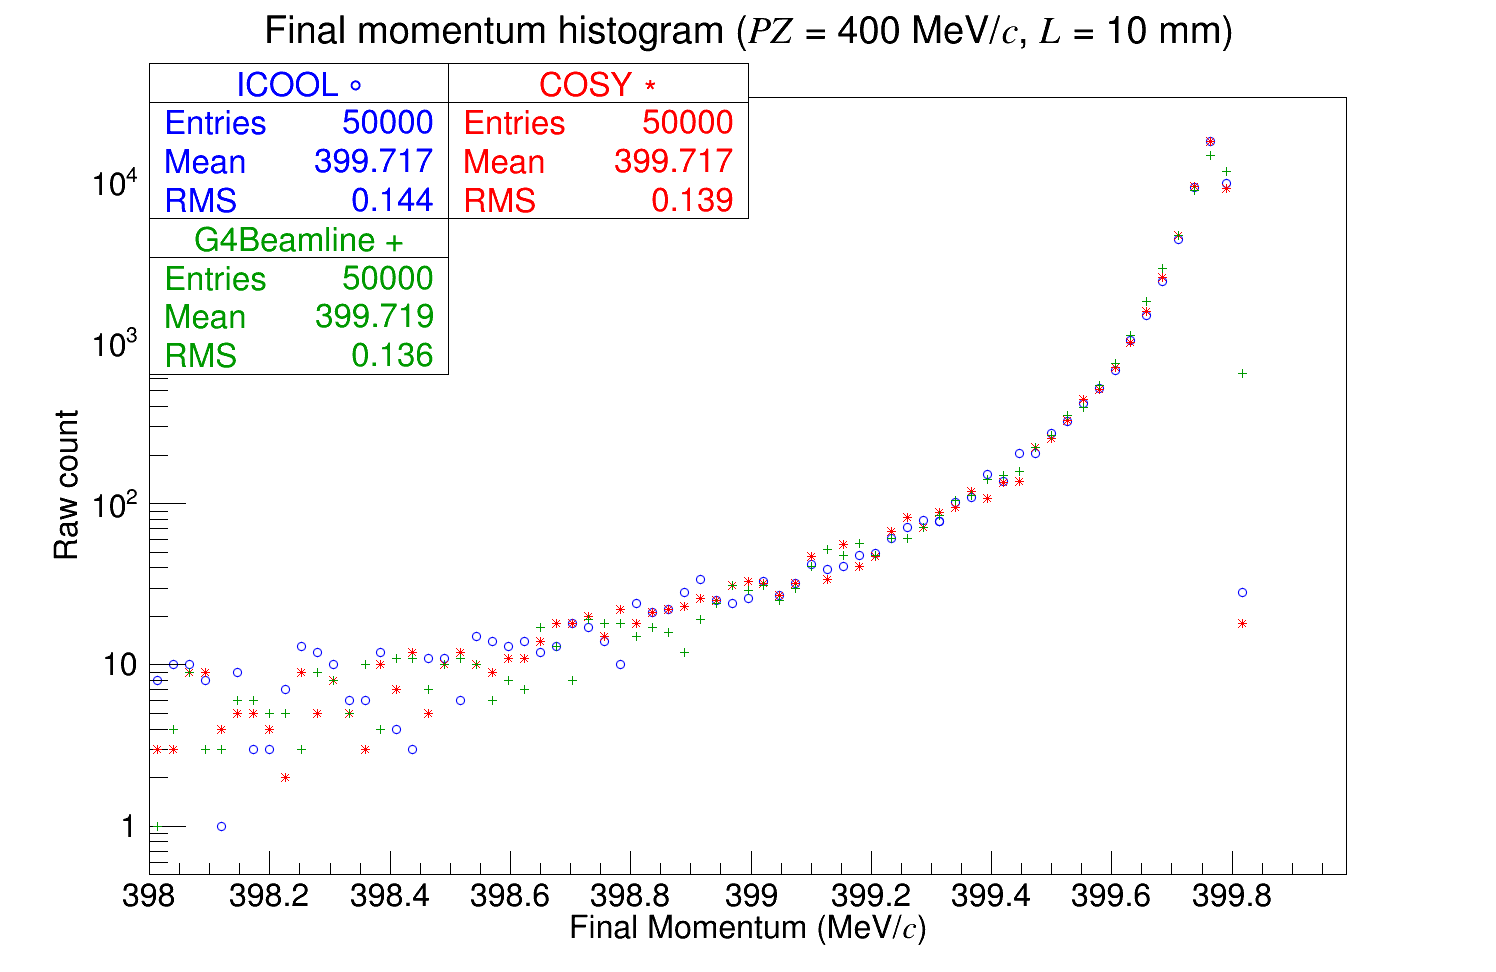
\includegraphics[width=0.7\textwidth]{Benchmarking/LH/strag.400.10.png} 
  \caption{Muons of momentum 400 MeV/$c$ through 10 mm liquid hydrogen.}
  \label{fig:400.10}
\end{figure}

\begin{figure}[H]
  \centering
    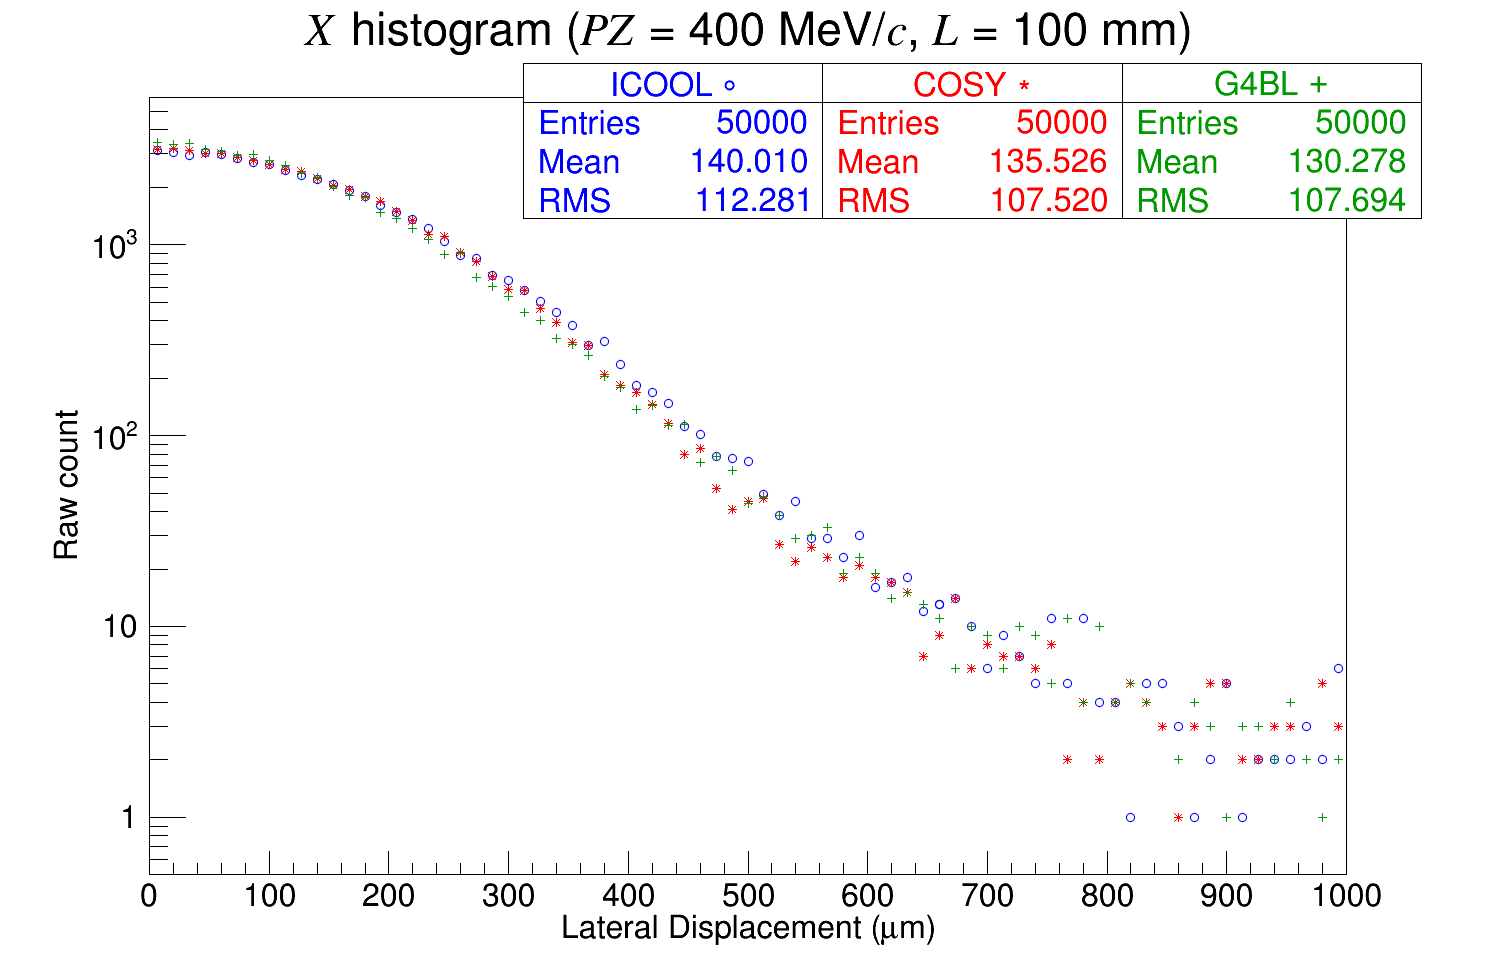
\includegraphics[width=0.7\textwidth]{Benchmarking/LH/X.400.100.png} 
    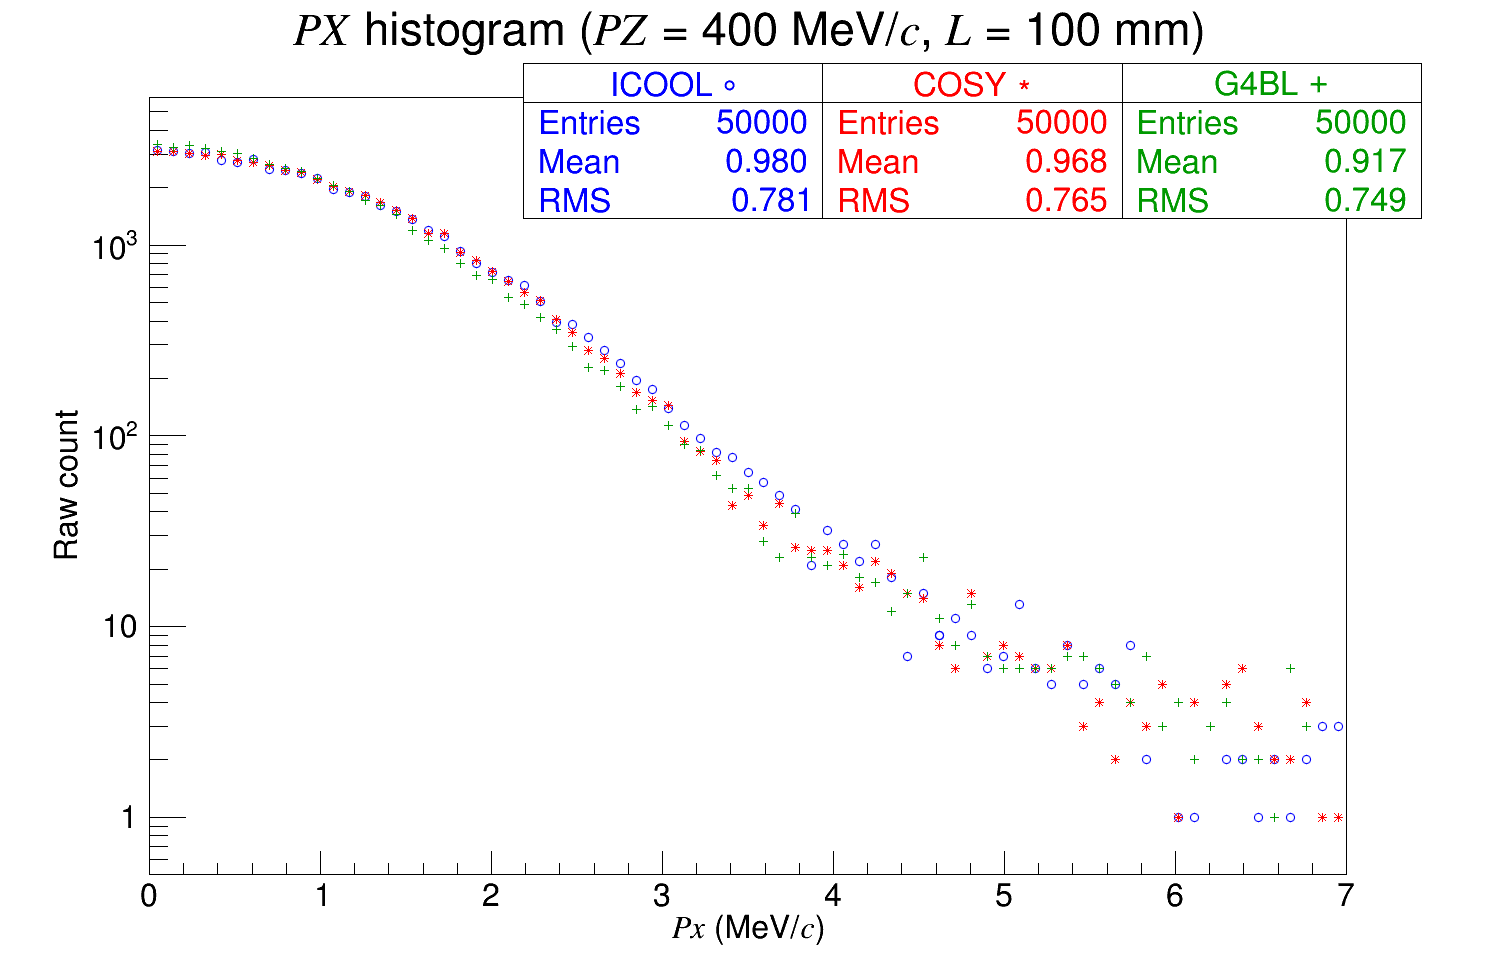
\includegraphics[width=0.7\textwidth]{Benchmarking/LH/PX.400.100.png} 
    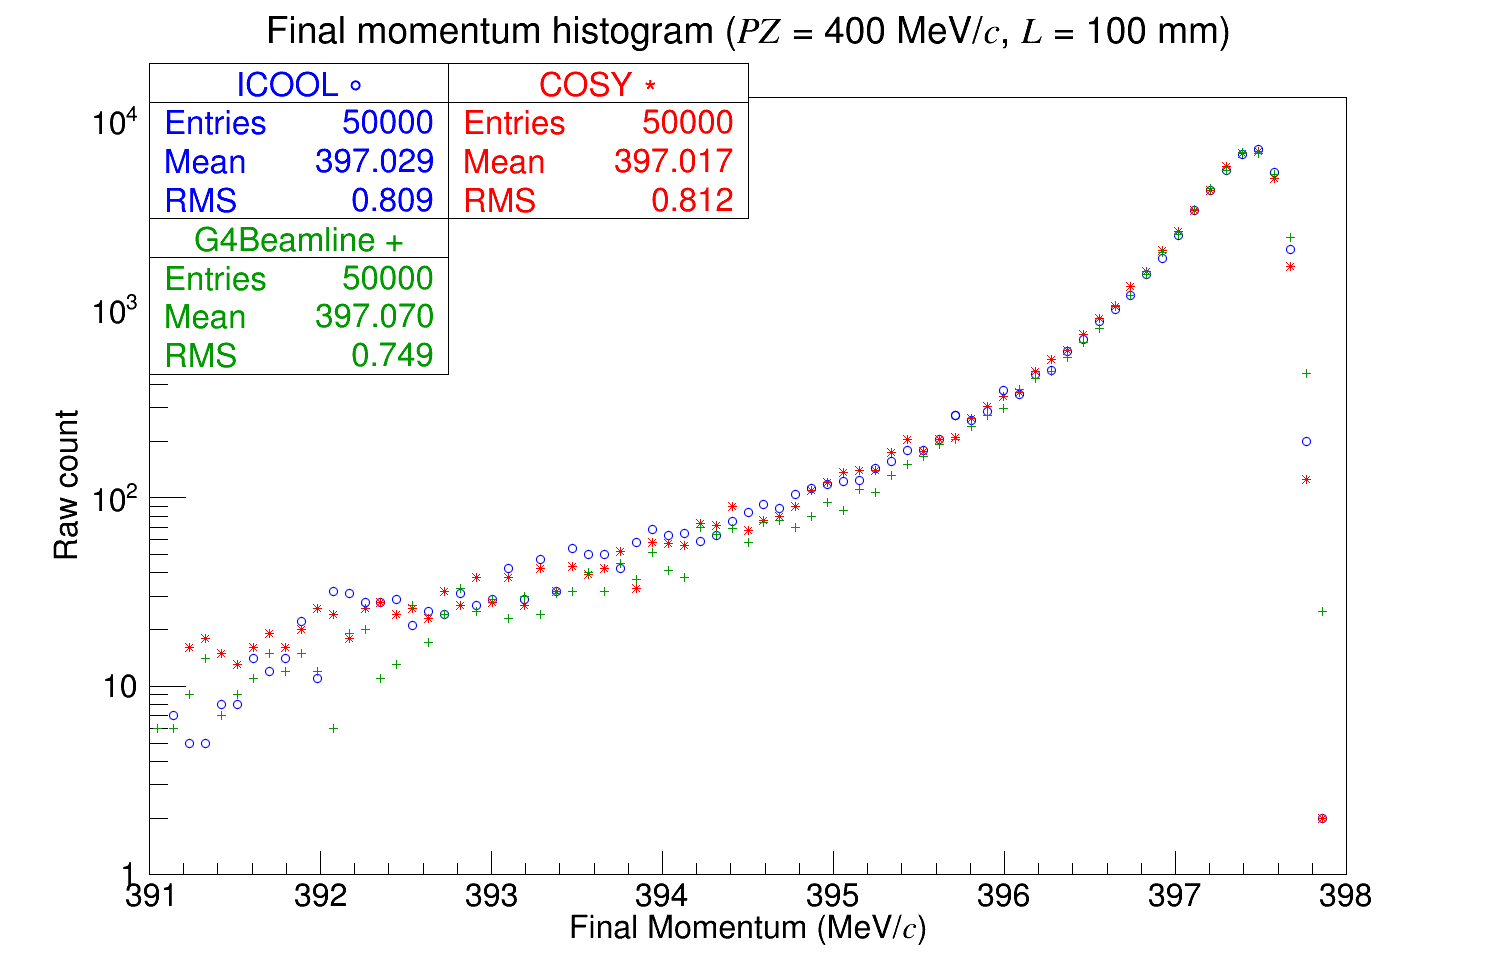
\includegraphics[width=0.7\textwidth]{Benchmarking/LH/strag.400.100.png} 
  \caption{Muons of momentum 400 MeV/$c$ through 100 mm liquid hydrogen.}
  \label{fig:400.100}
\end{figure}


For the 1 mm figures (Figures \ref{fig:100.1}, \ref{fig:200.1}, \ref{fig:300.1}, and \ref{fig:400.1}) there is much disagreement between the codes' transverse momentum distributions. Since the transverse momentum and transverse position coordinates are related, there is also disagreement among the transverse position distributions. This is likely because the default ICOOL scattering model uses a Fano peak with a Rutherford tail whereas both COSY and G4Beamline use a Gaussian peak. It can be seen by, e.g., Figure~\ref{fig:100.1} that COSY, like G4Beamline, uses the Gaussian model for the peak but, like ICOOL, then switches to a Rutherford tail.

For the 10 mm figures (Figures \ref{fig:100.10}, \ref{fig:200.10}, \ref{fig:300.10}, and \ref{fig:400.10}), both $x$ and $p_x$ distributions agree well. For COSY, the tail of the distribution falls off slightly faster after approximately 1~MeV/$c$. 

For the final momentum plots, ICOOL and COSY agree quite well. This is not surprising since both codes use Landau theory to describe the energy loss distribution. G4Beamline occasionally disagrees. An example of this can be seen in Figure~\ref{fig:200.1}. However, given the scale of the horizontal axis this disagreement is much smaller than it initially appears.

\Section{Validation}\label{sec:validation}

The new COSY routines were also compared to the Muon Scattering Experiment \cite{muscat}, often referred to as MuScat. This experiment measured the scattering of a beam of collimated muons through seven materials. To emulate this, pencil beams with momentum $P=172$ MeV/$c$ were created in COSY, G4Beamline, and ICOOL. The pencil beam consisted of $5\times10^6$ particles and was propagated through 109 mm of liquid hydrogen, 159 mm of liquid hydrogen, and 3.73 mm of beryllium. Liquid hydrogen was chosen to represent muons through long absorbers of low-$Z$ materials. Beryllium, on the other hand, was chosen to represent muons through much thinner and denser media. COSY took a single step through the absorbers while G4BL took a step size of 1 mm. The data points were normalized to the total probability, was calculated via Simpson's rule. The probability per radian was then found by dividing the probability of the data point by the scattered angle at that point. The results are shown below.

\begin{figure}[H]
  \centering
    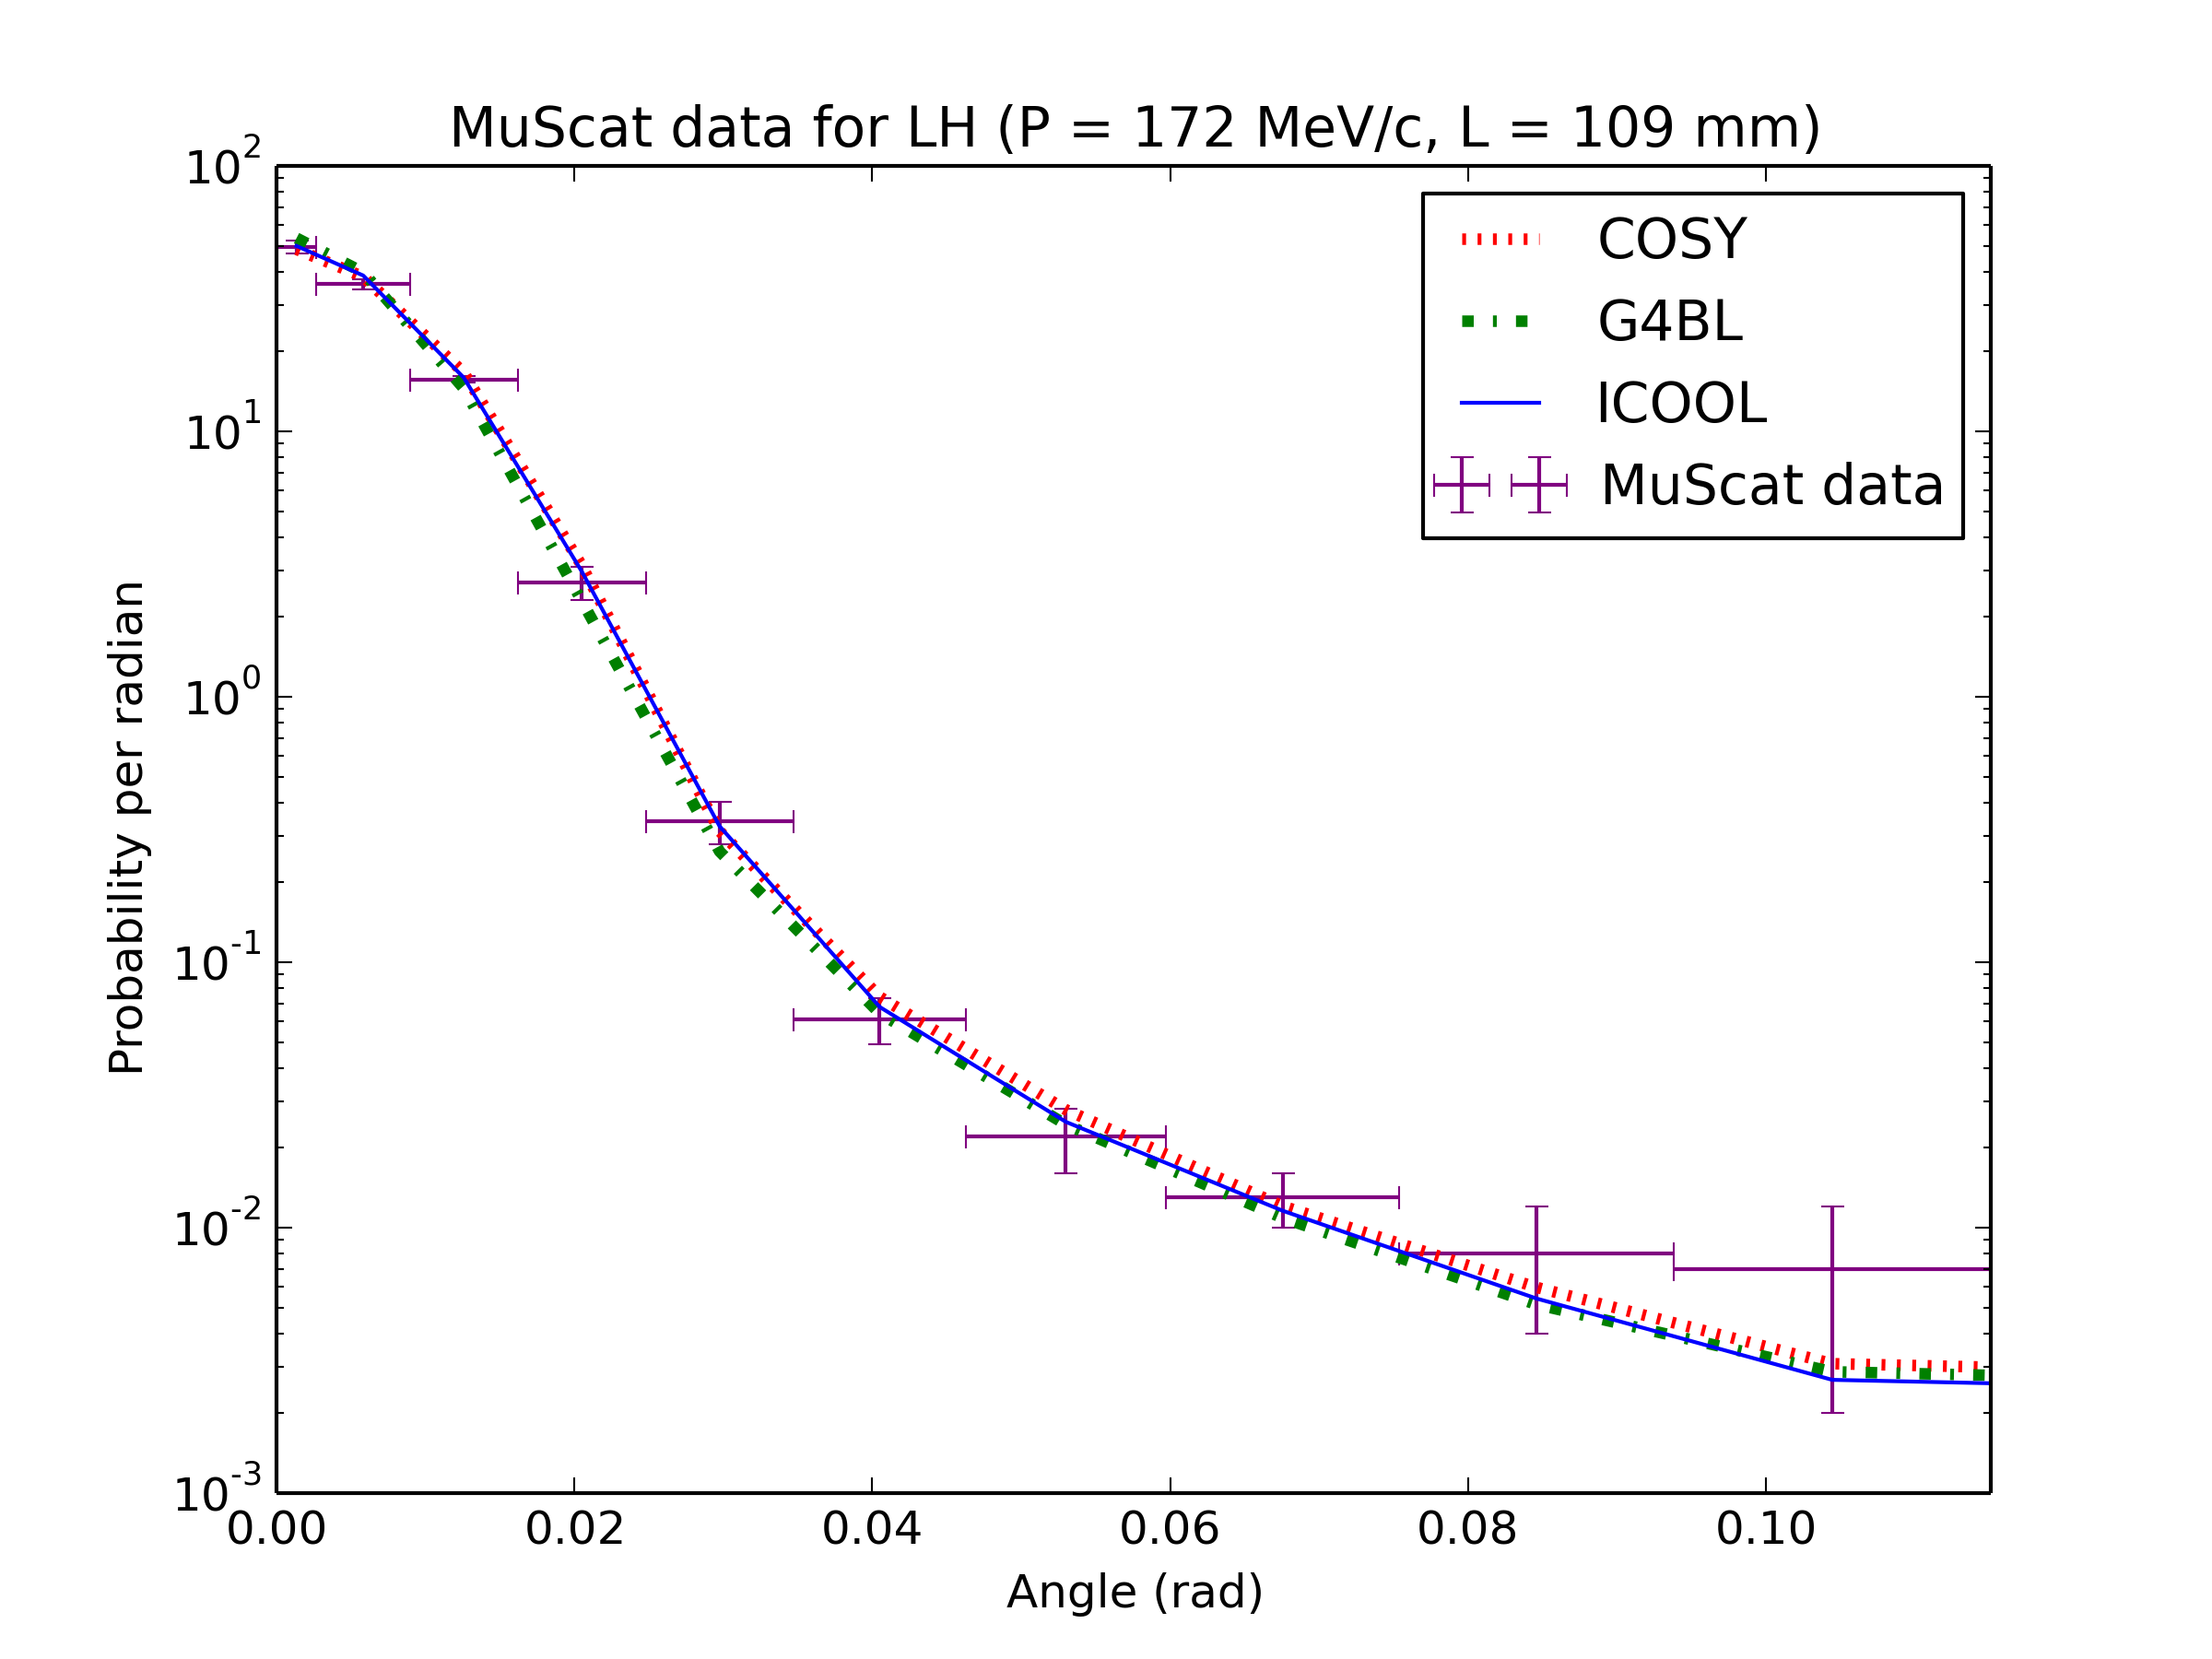
\includegraphics[width=\textwidth]{Figures/172.109.muscat} 
  \caption{MuScat angular scattering results for 109 mm of liquid hydrogen compared against COSY (red), G4BL (green), and ICOOL (blue).}
  \label{fig:172.109.muscat}
\end{figure}

\begin{figure}[H]
  \centering
    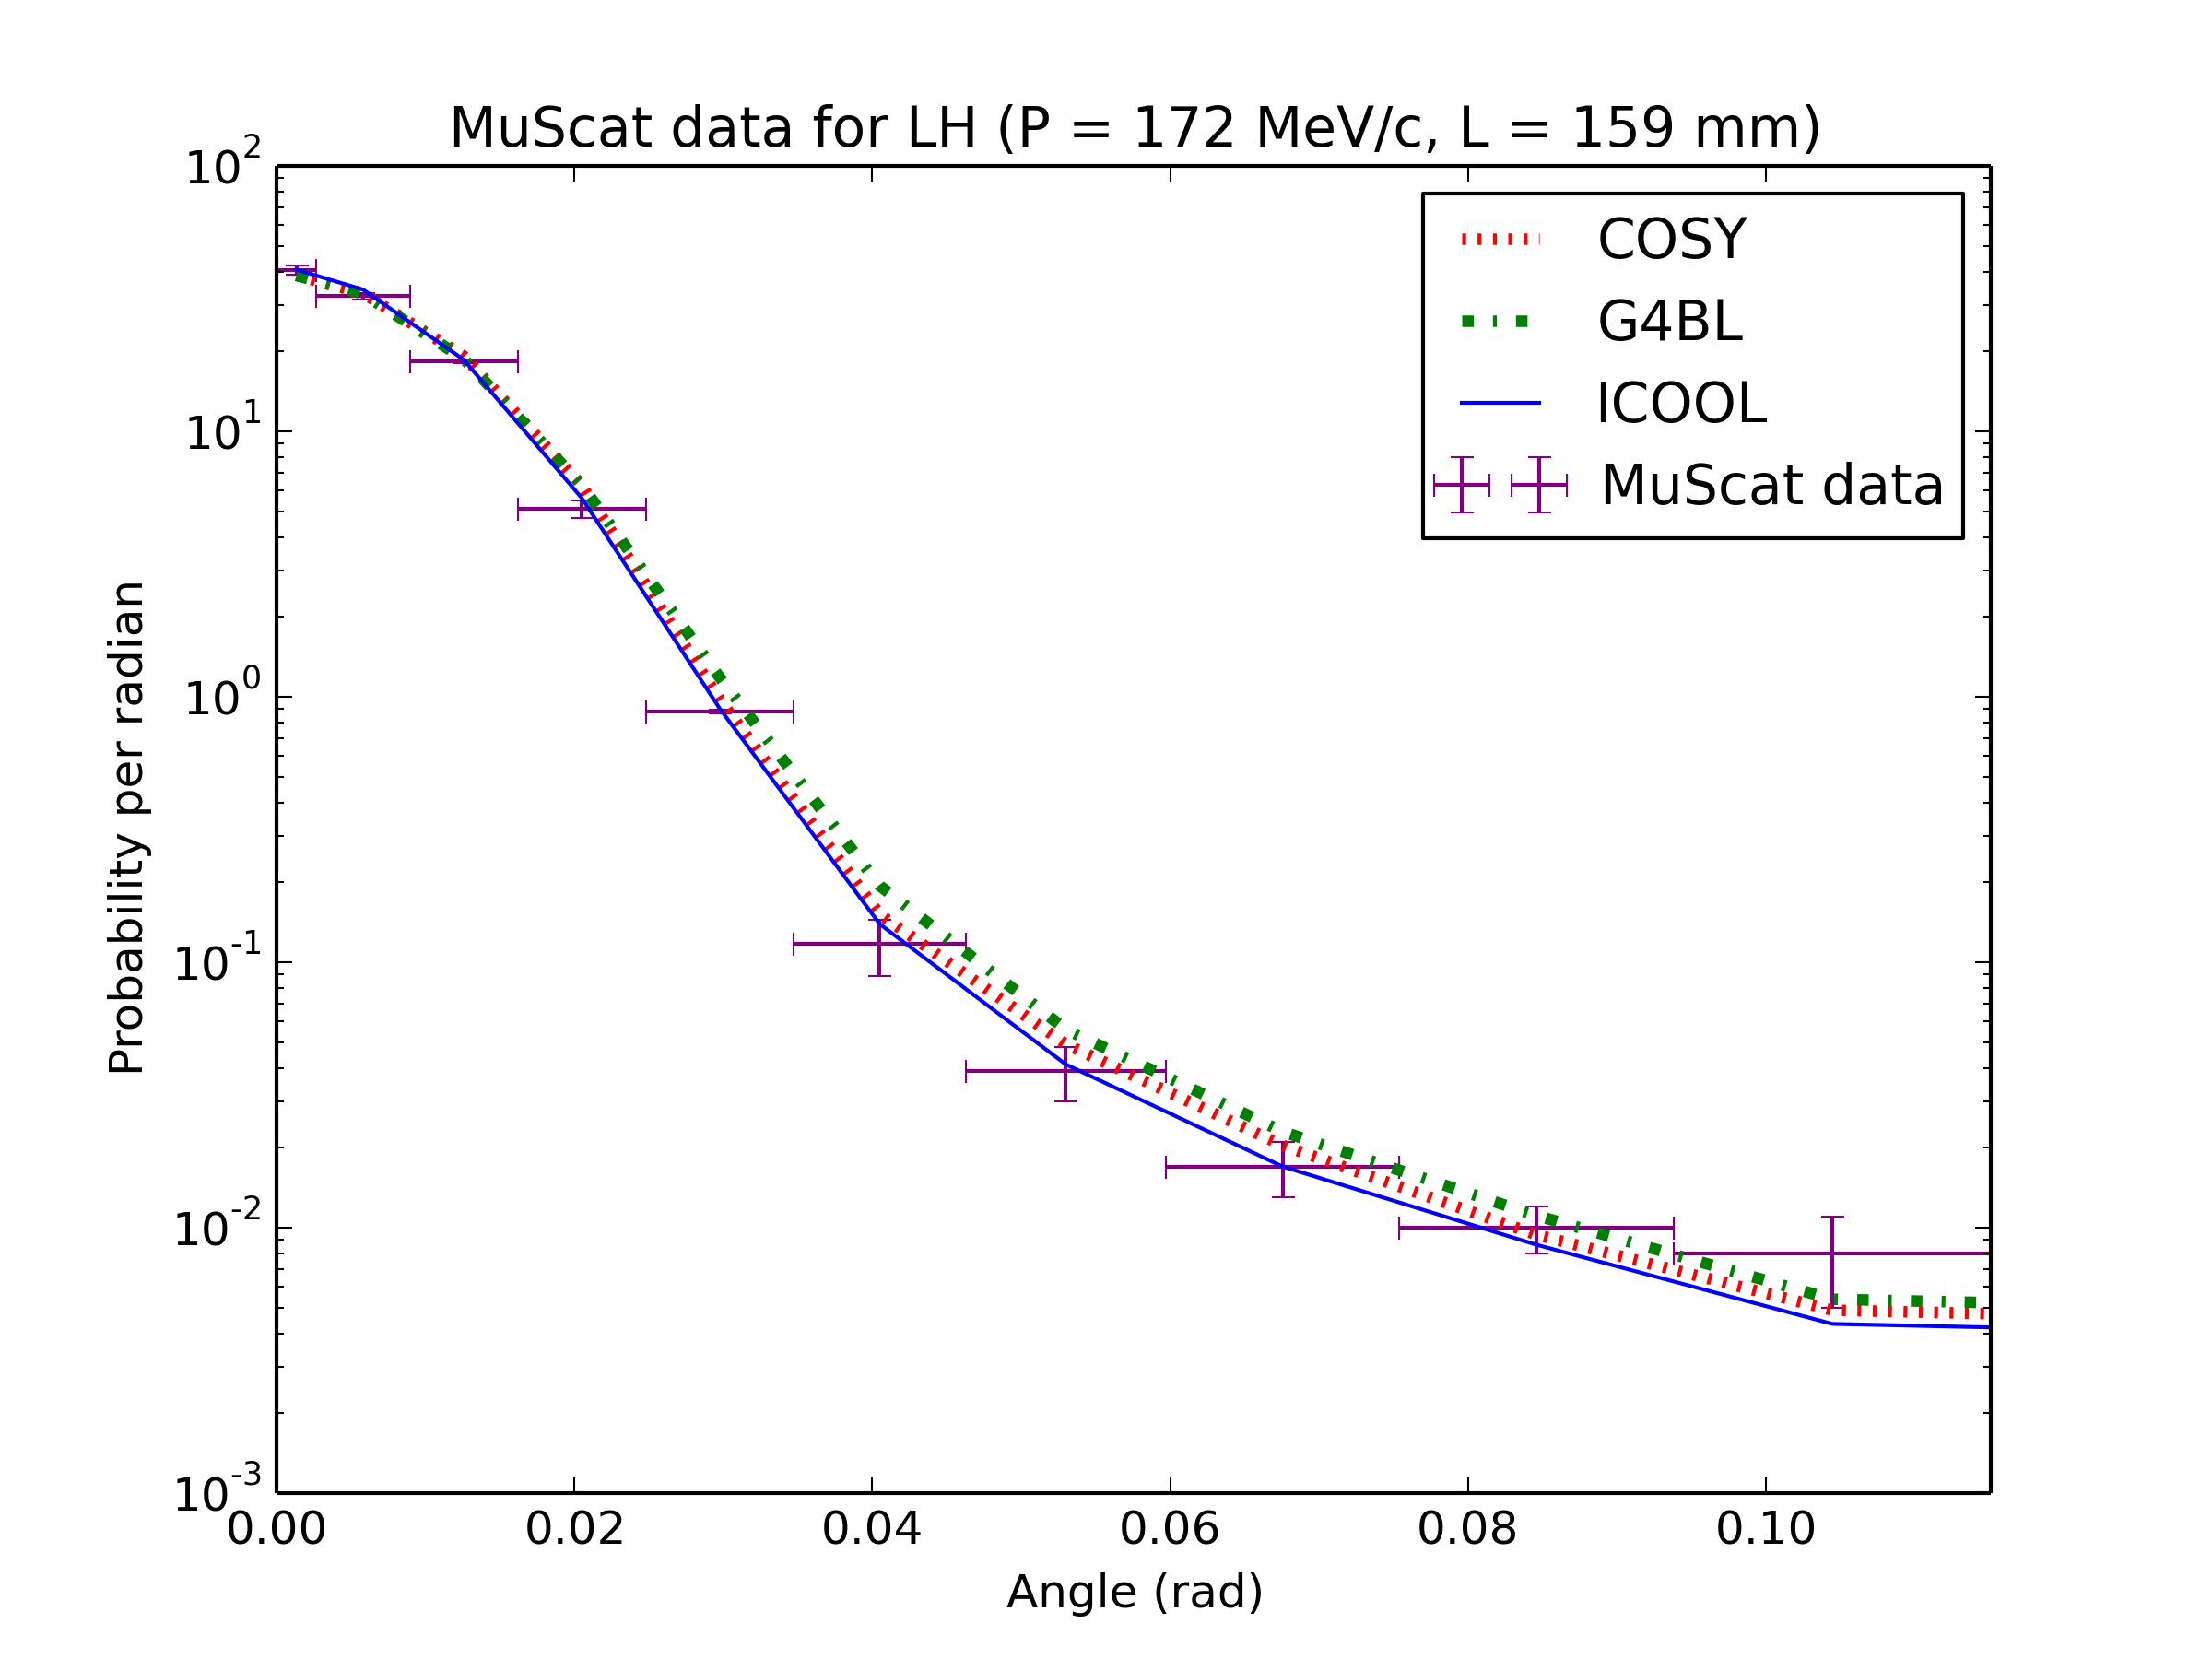
\includegraphics[width=\textwidth]{Figures/172.159.muscat} 
  \caption{MuScat angular scattering results for 159 mm of liquid hydrogen compared against COSY (red), G4BL (green), and ICOOL (blue).}
  \label{fig:172.159.muscat}
\end{figure}

\begin{figure}[H]
  \centering
    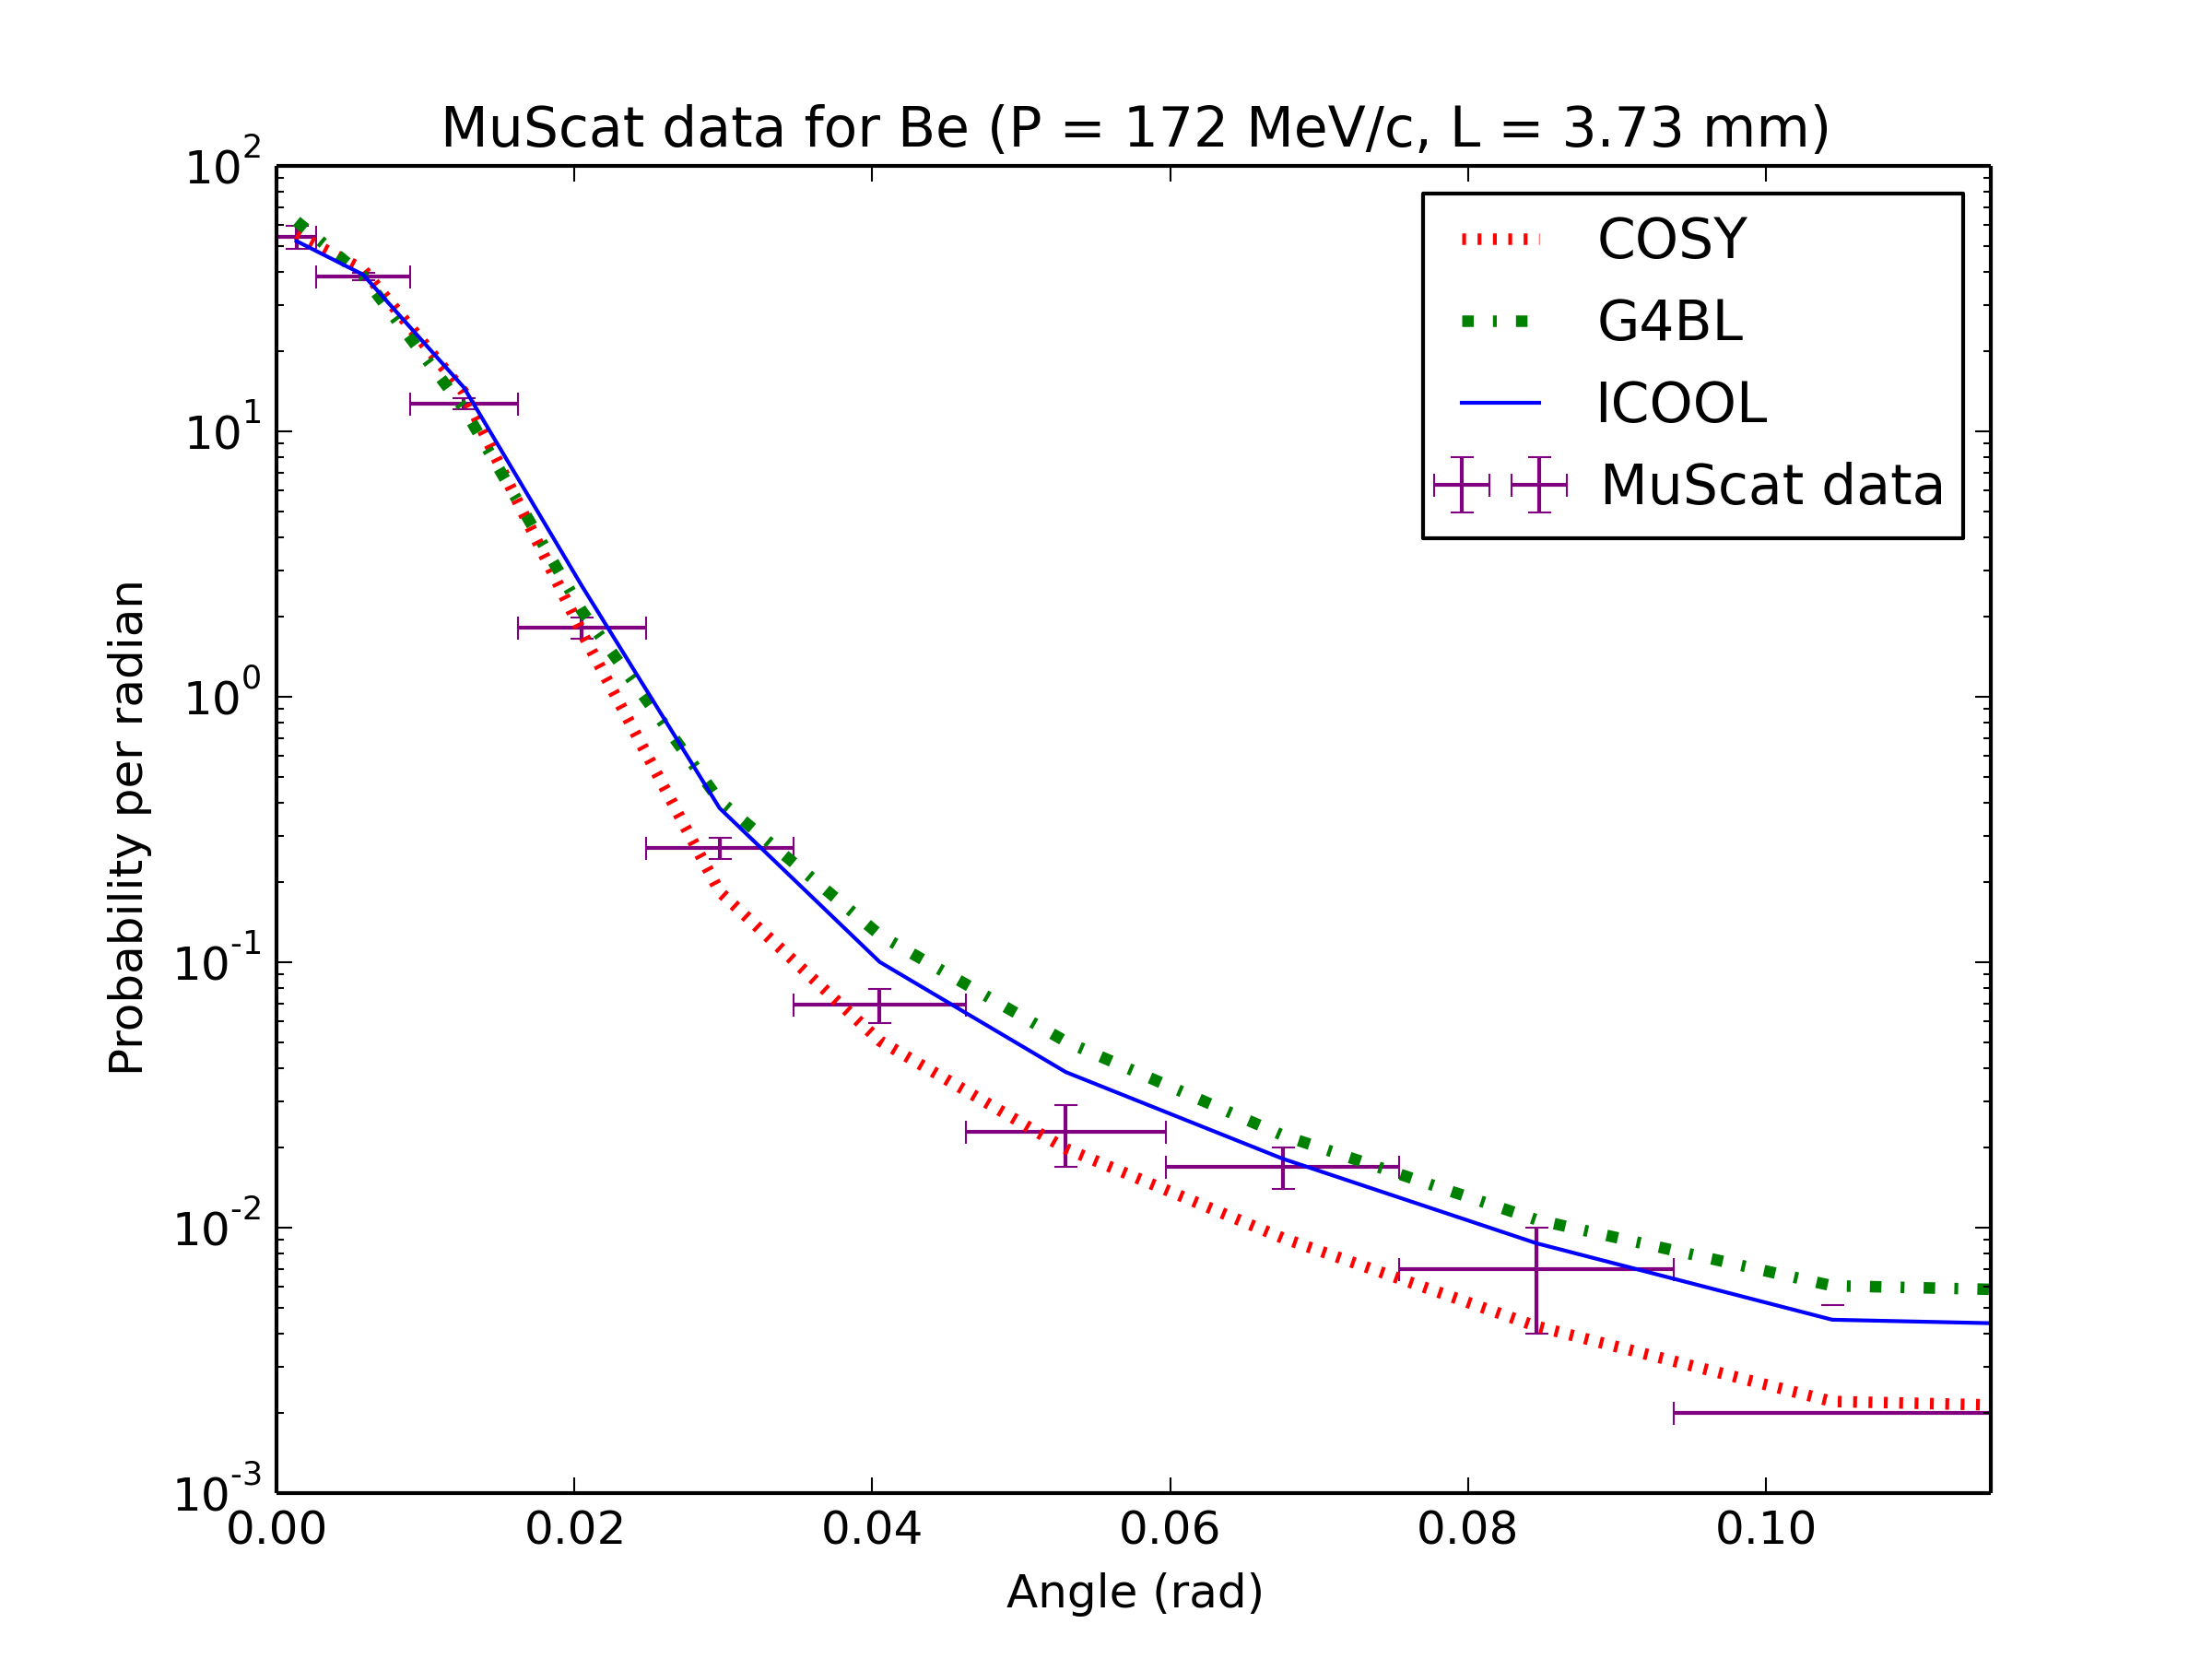
\includegraphics[width=\textwidth]{Figures/172.3.73.muscat} 
  \caption{MuScat angular scattering results for 3.73 mm of beryllium compared against COSY (red), G4BL (green), and ICOOL (blue).}
  \label{fig:172.3.73.muscat}
\end{figure}

In the liquid hydrogen cases, COSY appears to match both G4Beamline and ICOOL very well, as well as the MuScat data points. ICOOL appears to have a sharper peak than either COSY or G4Beamline, which can be more easily seen in the 159 mm liquid hydrogen case than in the 109 mm case. In the case of beryllium, COSY matches the MuScat points slightly better than G4Beamline and ICOOL, particularly for the two data points between 0.04 and 0.06 radians.

\Section{The Muon Ionization Cooling Experiment}\label{sec:mice}

This section introduces the Muon Ionization Cooling Experiment (MICE, \cite{mice}), a practical application for the new absorber routines in COSY. The results of MICE simulations in ICOOL, G4Beamline, and COSY are examined, showing good agreement.

\Subsection{Introduction to MICE}\label{ssc:miceIntro}
The Muon Ionization Cooling Experiment (MICE \cite{mice}) is an experiment currently being developed at the Rutherford Appleton Laboratory in Oxfordshire, U.K. Its goal is to show a proof-of-principle demonstration of muon ionization cooling. MICE Step IV configuration is explored in this work. The Step IV cell includes 12 magnetic coils positioned symmetrically around a flat absorber. Figure~\ref{fig:miceStepIV} shows a schematic of this lattice with 350 mm of liquid hydrogen as the absorber.
\begin{figure}[h!]
  \centering
    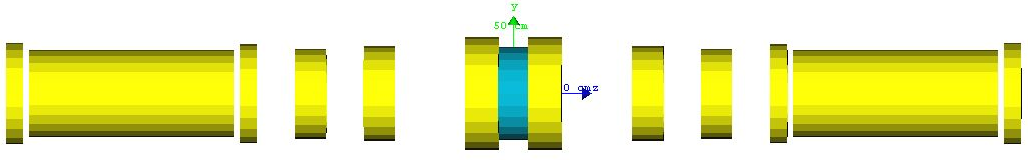
\includegraphics[width=\textwidth]{Figures/miceStepIV} 
  \caption[MICE Step IV cell.]{MICE Step IV cell. Magnetic coils are shown in yellow and the absorber is shown in blue. The green and blue axes are the $y$ and $z$ axes, here drawn to scale as 50 cm each. Image rendered via G4Beamline \cite{g4bl}.}
  \label{fig:miceStepIV}
\end{figure}

\Subsection{Results of MICE Simulation}\label{ssc:miceResults}
$10^6$ muons were simulated through the cell in Figure~\ref{fig:miceStepIV}. The coil parameters may be found in Table~\ref{tbl:MICE_coil_parameters}. The absorber was a 350 mm cylindrical block of liquid hydrogen centered at $z=0$. Note that other materials such as safety windows were not accounted for in this simulation. The decay process was disabled in all simulation codes. The beam started at $-$2.45105 m and ended at 2.450 m. The initial distribution was Gaussian with parameters summarized in Table~\ref{tbl:MICE_initial_distribution_parameters}.

\begin{table}
\caption*{\textbf{MICE Step IV Coil Parameters}}
\begin{tabularx}{\textwidth}{cccccccc}
\hline \hline
Name & $z$ position & Length & Inner radius & Outer radius & Current density  \vspace{-12pt}\\
 & mm & mm & mm & mm & A/mm$^2$  \\
\hline
	End2 & $\mp$3200.28&110.642&258&325.783&$\pm$126 \vspace{-12pt}\\
	Center&$\mp$2450.275&1314.3&258&280.125&$\pm$148 \vspace{-12pt}\\
	End1 & $\mp$1700.29& 110.642& 258 & 318.905 & $\pm$133 \vspace{-12pt}\\
	Match2 & $\mp$1300.29 & 199.492 & 258 & 288.925 & $\pm$132 \vspace{-12pt}\\
	Match1 & $\mp$860.645 & 201.268 & 258 & 304.165 & $\pm133$ \vspace{-12pt}\\
	Focus & $\mp$202.2 & 213.3 & 267.6 & 361.9 & $\pm$104 \\ 
\hline
\end{tabularx}
\caption[MICE Step IV coil parameters.]{MICE Step IV coil parameters corresponding to Figure~\ref{fig:miceStepIV}.}
\label{tbl:MICE_coil_parameters}
\end{table}

%\newcolumntype{A}{ >{\centering\arraybackslash} m{2.5cm} } 
\begin{table}
\caption*{\textbf{MICE Step IV Initial Distribution Parameters}}
\begin{center}
\begin{tabularx}{0.7\textwidth}{p{1cm}ccc}
\hline \hline
&Parameter & Mean & Standard deviation \\
\hline
	&$x$ (mm) & 0 & 32\vspace{-12pt}\\
	&$y$ (mm) & 0 & 32\vspace{-12pt} \\
	&$z$ (mm) & 0 & 0\vspace{-12pt} \\
	&$p_x$ (MeV/$c$) & 0 & 20\vspace{-12pt} \\
	&$p_y$ (MeV/$c$) & 0 & 20\vspace{-12pt} \\
	&$p_z$ (MeV/$c$) & 200 & 30\\
\hline
\end{tabularx}
\end{center}
\caption{MICE Step IV initial distribution Gaussian parameters.}
\label{tbl:MICE_initial_distribution_parameters}
\end{table}

For COSY, it was found that a 5th order simulation was sufficient. Through the coil-only portion of the simulation, 100 steps were taken on each side of the absorber (or roughly a step size of 24.5 mm both upstream and downstream). The selection of order and step size are detailed in the next section. The particles were tracked through the momentary tranfer map after each step and then the transfer map was set to unity. It was noted that for the coil-only section, a single transfer map was not sufficient even at the 21st order. This is likely due to the large phase space volume of the initial beam and the complexity of the magnetic field.

Compounding the map without propagating the beam also gave poor results. When one takes the composition of two $n^{th}$ order transfer maps, a transfer map of order $n\times n$ is the result. For example, the first step in MICE simulation would yield a 3rd order transfer map. Taking the second step would give a new transfer map of order $3\times 3 = 9$. However, since COSY is operating in the 3rd order mode, the new transfer map would not be 9th order, but rather it would be truncated to a 3rd order map. For this reason, the particles were propagated through the momentary transfer map after each step in the simulation.

When the beam entered the region of the absorber, COSY switched to a step size of 10 mm in order to simulate the superposition of the magnetic coils and the absorber.

The magnetic field in G4Beamline was created using the \texttt{coil} and \texttt{solenoid} commands. The field was then exported to a file using the \texttt{printfield} command so that ICOOL could read and create its own field map via the \texttt{GRID} command operating in \texttt{G43D} mode.

\begin{figure}[H]
  \centering
    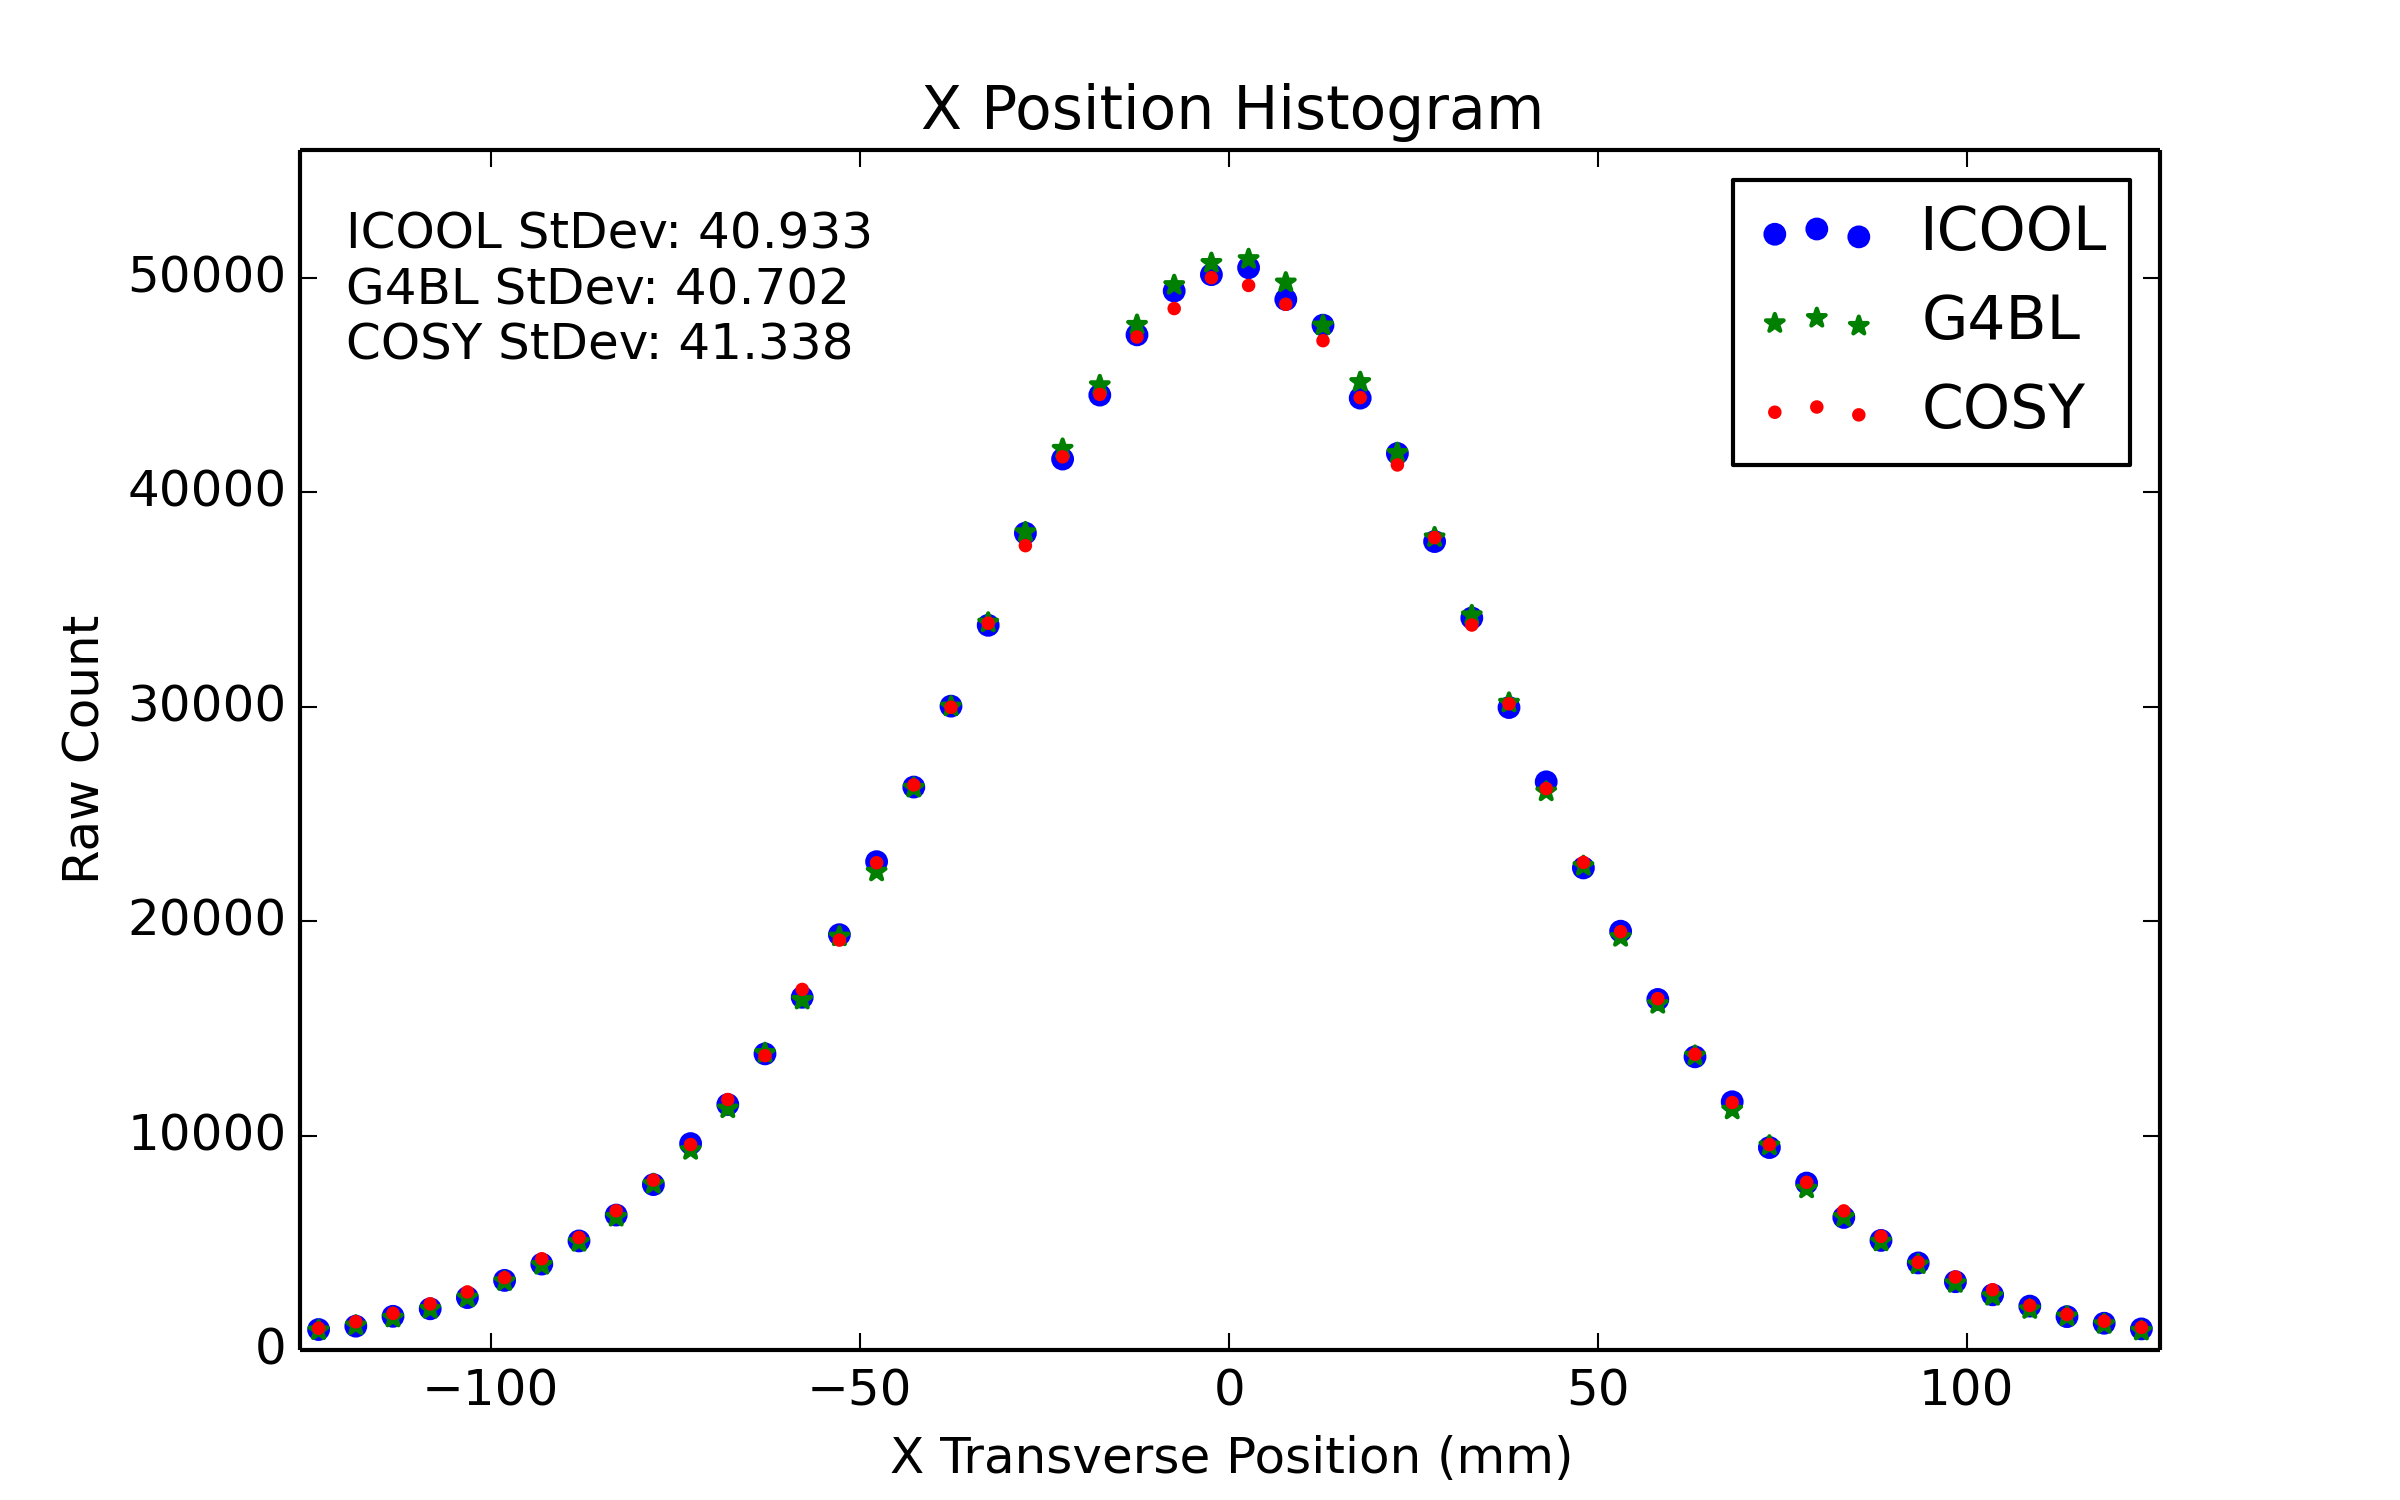
\includegraphics[width=\textwidth]{MICE data/x} 
  \caption{MICE Step IV $x$ position results for 350 mm of liquid hydrogen.}
  \label{fig:micex}
\end{figure}

\begin{figure}[H]
  \centering
    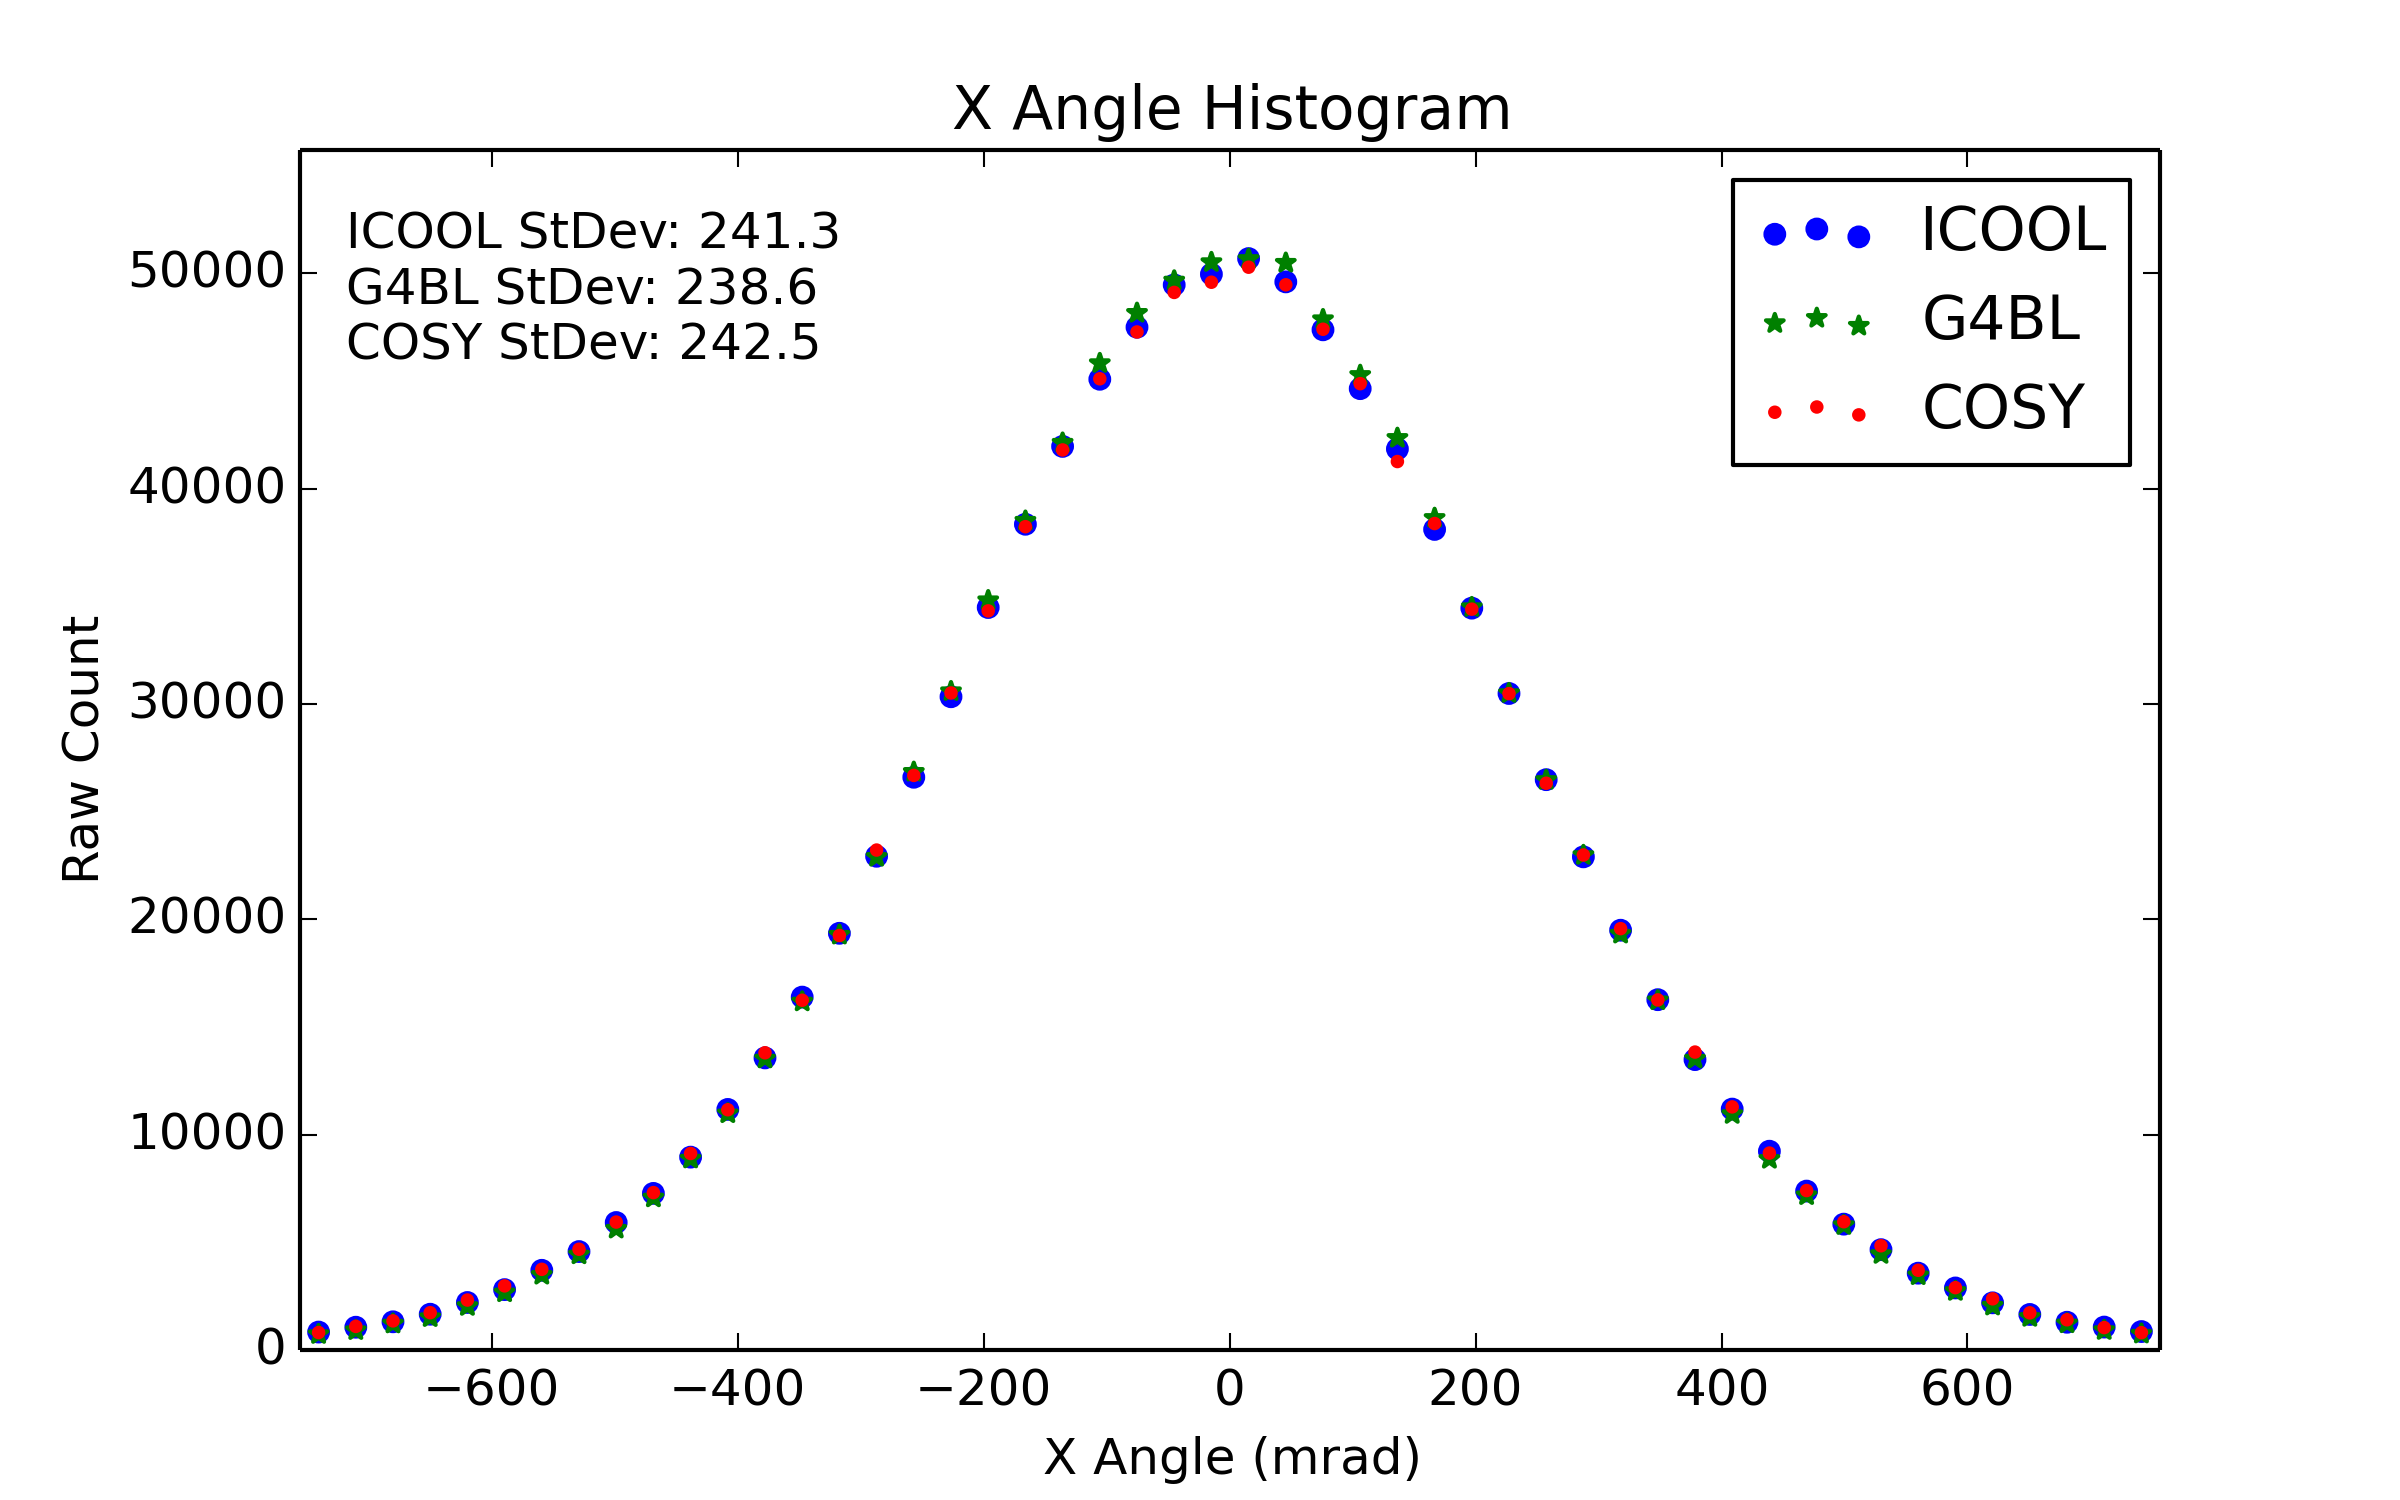
\includegraphics[width=\textwidth]{MICE data/px} 
  \caption{MICE Step IV $x$ angle results for 350 mm of liquid hydrogen.}
  \label{fig:micexangle}
\end{figure}

\begin{figure}[H]
  \centering
    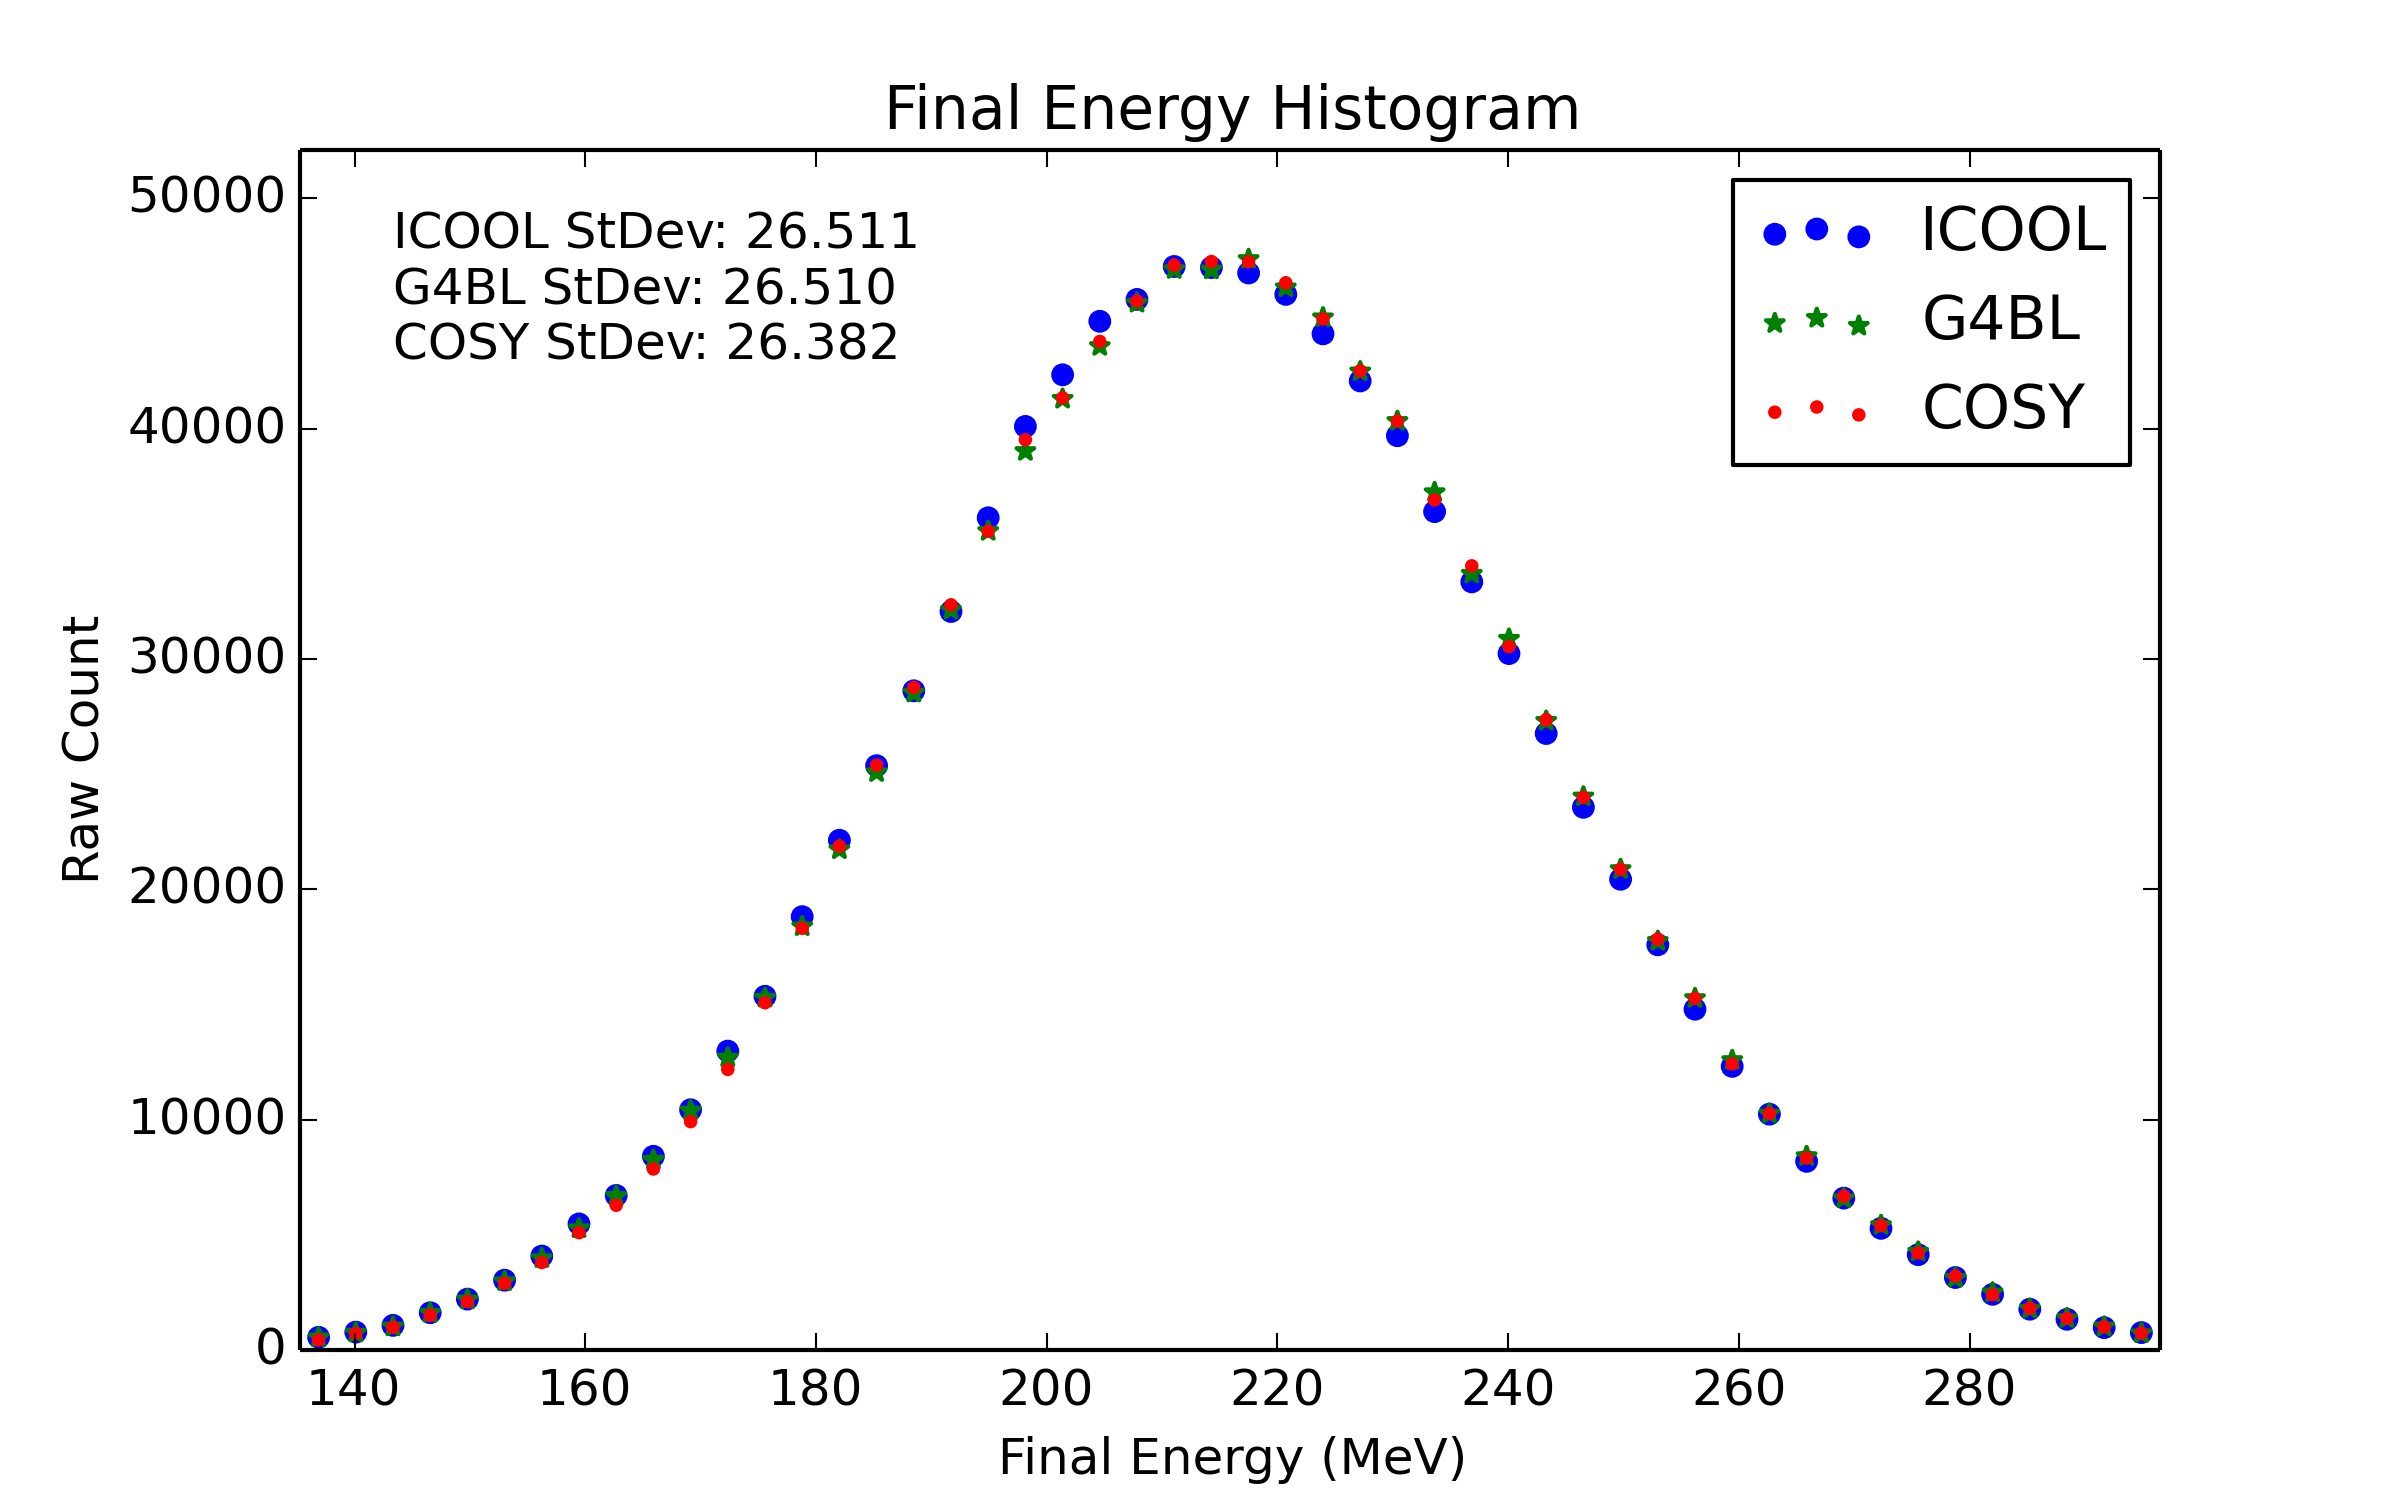
\includegraphics[width=\textwidth]{MICE data/e} 
  \caption{MICE Step IV final energy results for 350 mm of liquid hydrogen.}
  \label{fig:miceenergy}
\end{figure}

The runtimes of ICOOL, G4Beamline, and COSY are listed in Table~\ref{tbl:mice_times}. To reiterate, COSY was run at 5th order with 100 steps before the absorber, 350 steps inside the absorber, and 100 steps after the absorber. Note that the initialization time for G4Beamline to create the field maps was 33 seconds. However, since G4Beamline only has to create the field map once, the initialization time is not added to the run times in Table~\ref{tbl:mice_times}.

\begin{table}
\caption*{\textbf{Run Times (in seconds) for MICE Step IV Simulation}}
\begin{center}
\begin{tabularx}{0.6\textwidth}{ccccc}
%\vspace{-40pt}\\ 
\hline \hline
Number of particles: & $10^6$ & $10^5$ & $10^4$ & $10^3$\\
\hline
ICOOL: & 533 & 49 & 12 & 9\vspace{-12pt}\\
G4Beamline: & 3973 & 392 & 40 & 6\vspace{-12pt}\\
COSY: & 893 & 73 & 13 & 7\\
\hline
\end{tabularx}
\end{center}
\caption[Run times for MICE Step IV simulation.]{Run times for MICE Step IV simulation for liquid hydrogen. Note that the G4Beamline initialization time was not added to the run time values.}
\label{tbl:mice_times}
\end{table}

As a second test, MICE configuration in Figure~\ref{fig:miceStepIV} was simulated using 65 mm of lithium hydride. Lithium hydride is an attractive material because, unlike liquid hydrogen, it does not require cryogenic conditions, but still maintains a low $Z$ value. It can be seen from Figures \ref{fig:mice_lih_x}, \ref{fig:mice_lih_xangle}, and \ref{fig:mice_lih_energy} that 65 mm of lithium hydride has a similar effect on the beam as 350 mm of liquid hydrogen. It should be noted that inside the absorber, a 5 mm step size was chosen instead of a 10 mm step size (since 10 does not evenly go into 65).

\begin{figure}[H]
  \centering
    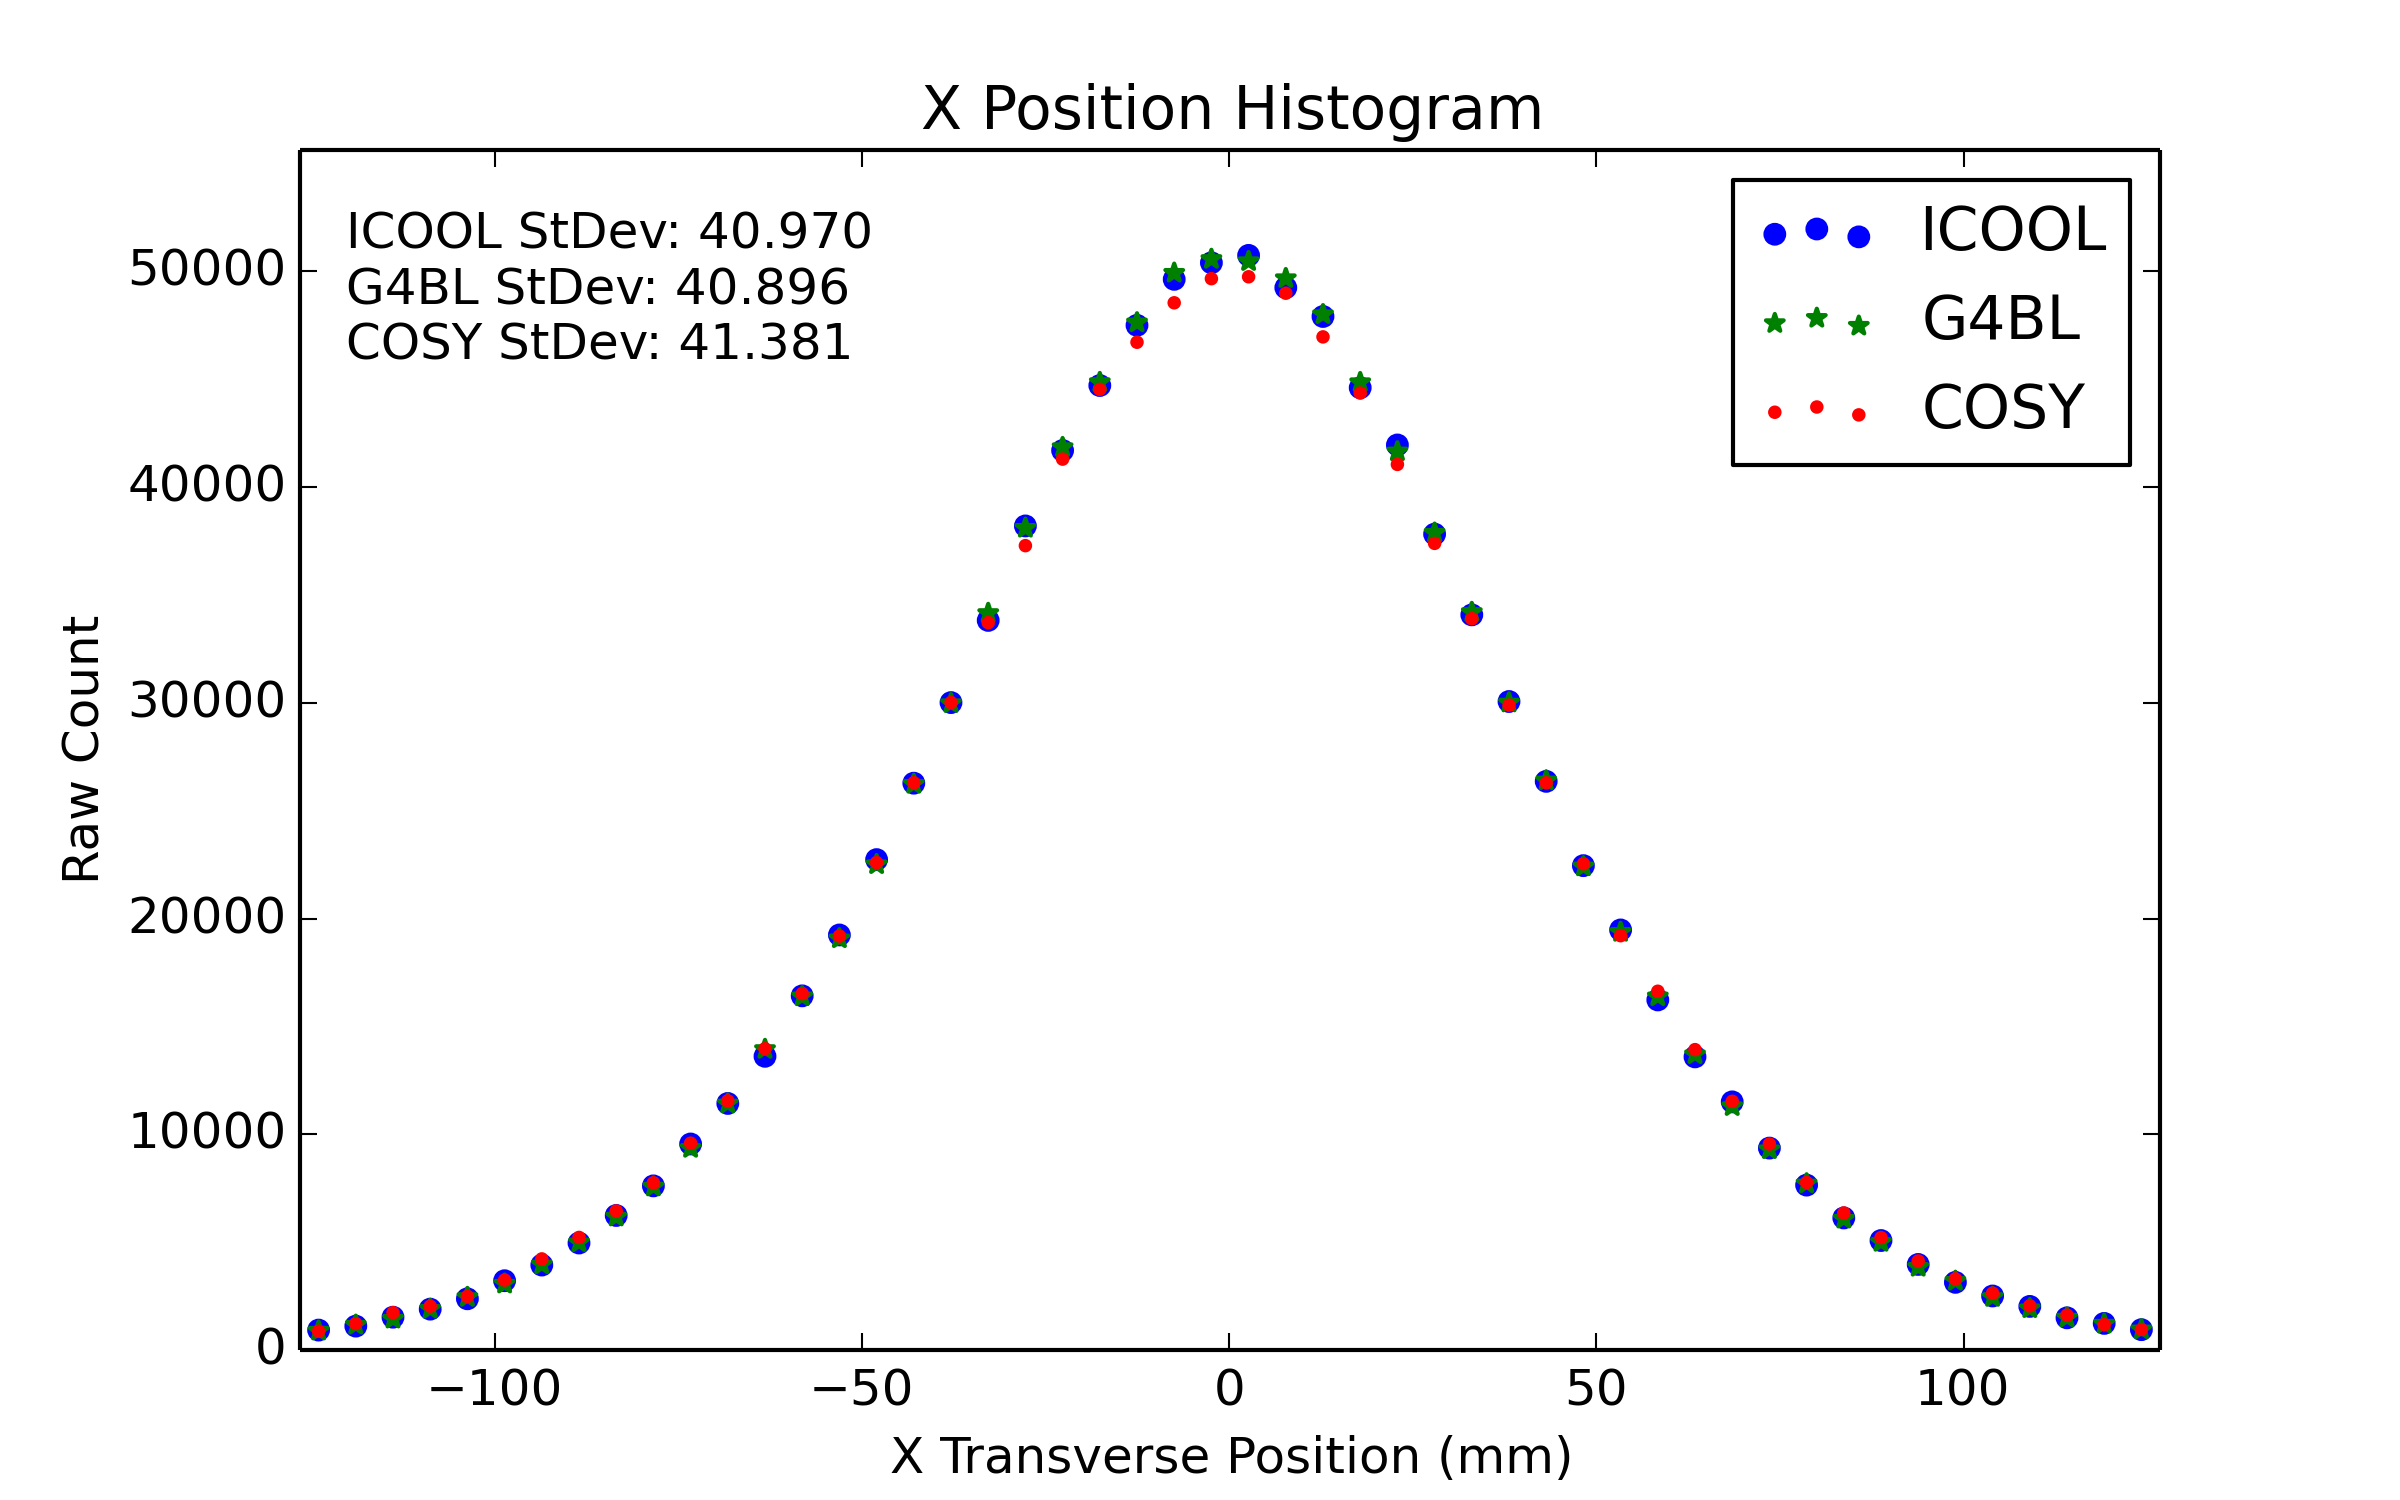
\includegraphics[width=\textwidth]{MICE data/LiH/x} 
  \caption{MICE Step IV $x$ position results for 65 mm of lithium hydride.}
  \label{fig:mice_lih_x}
\end{figure}

\begin{figure}[H]
  \centering
    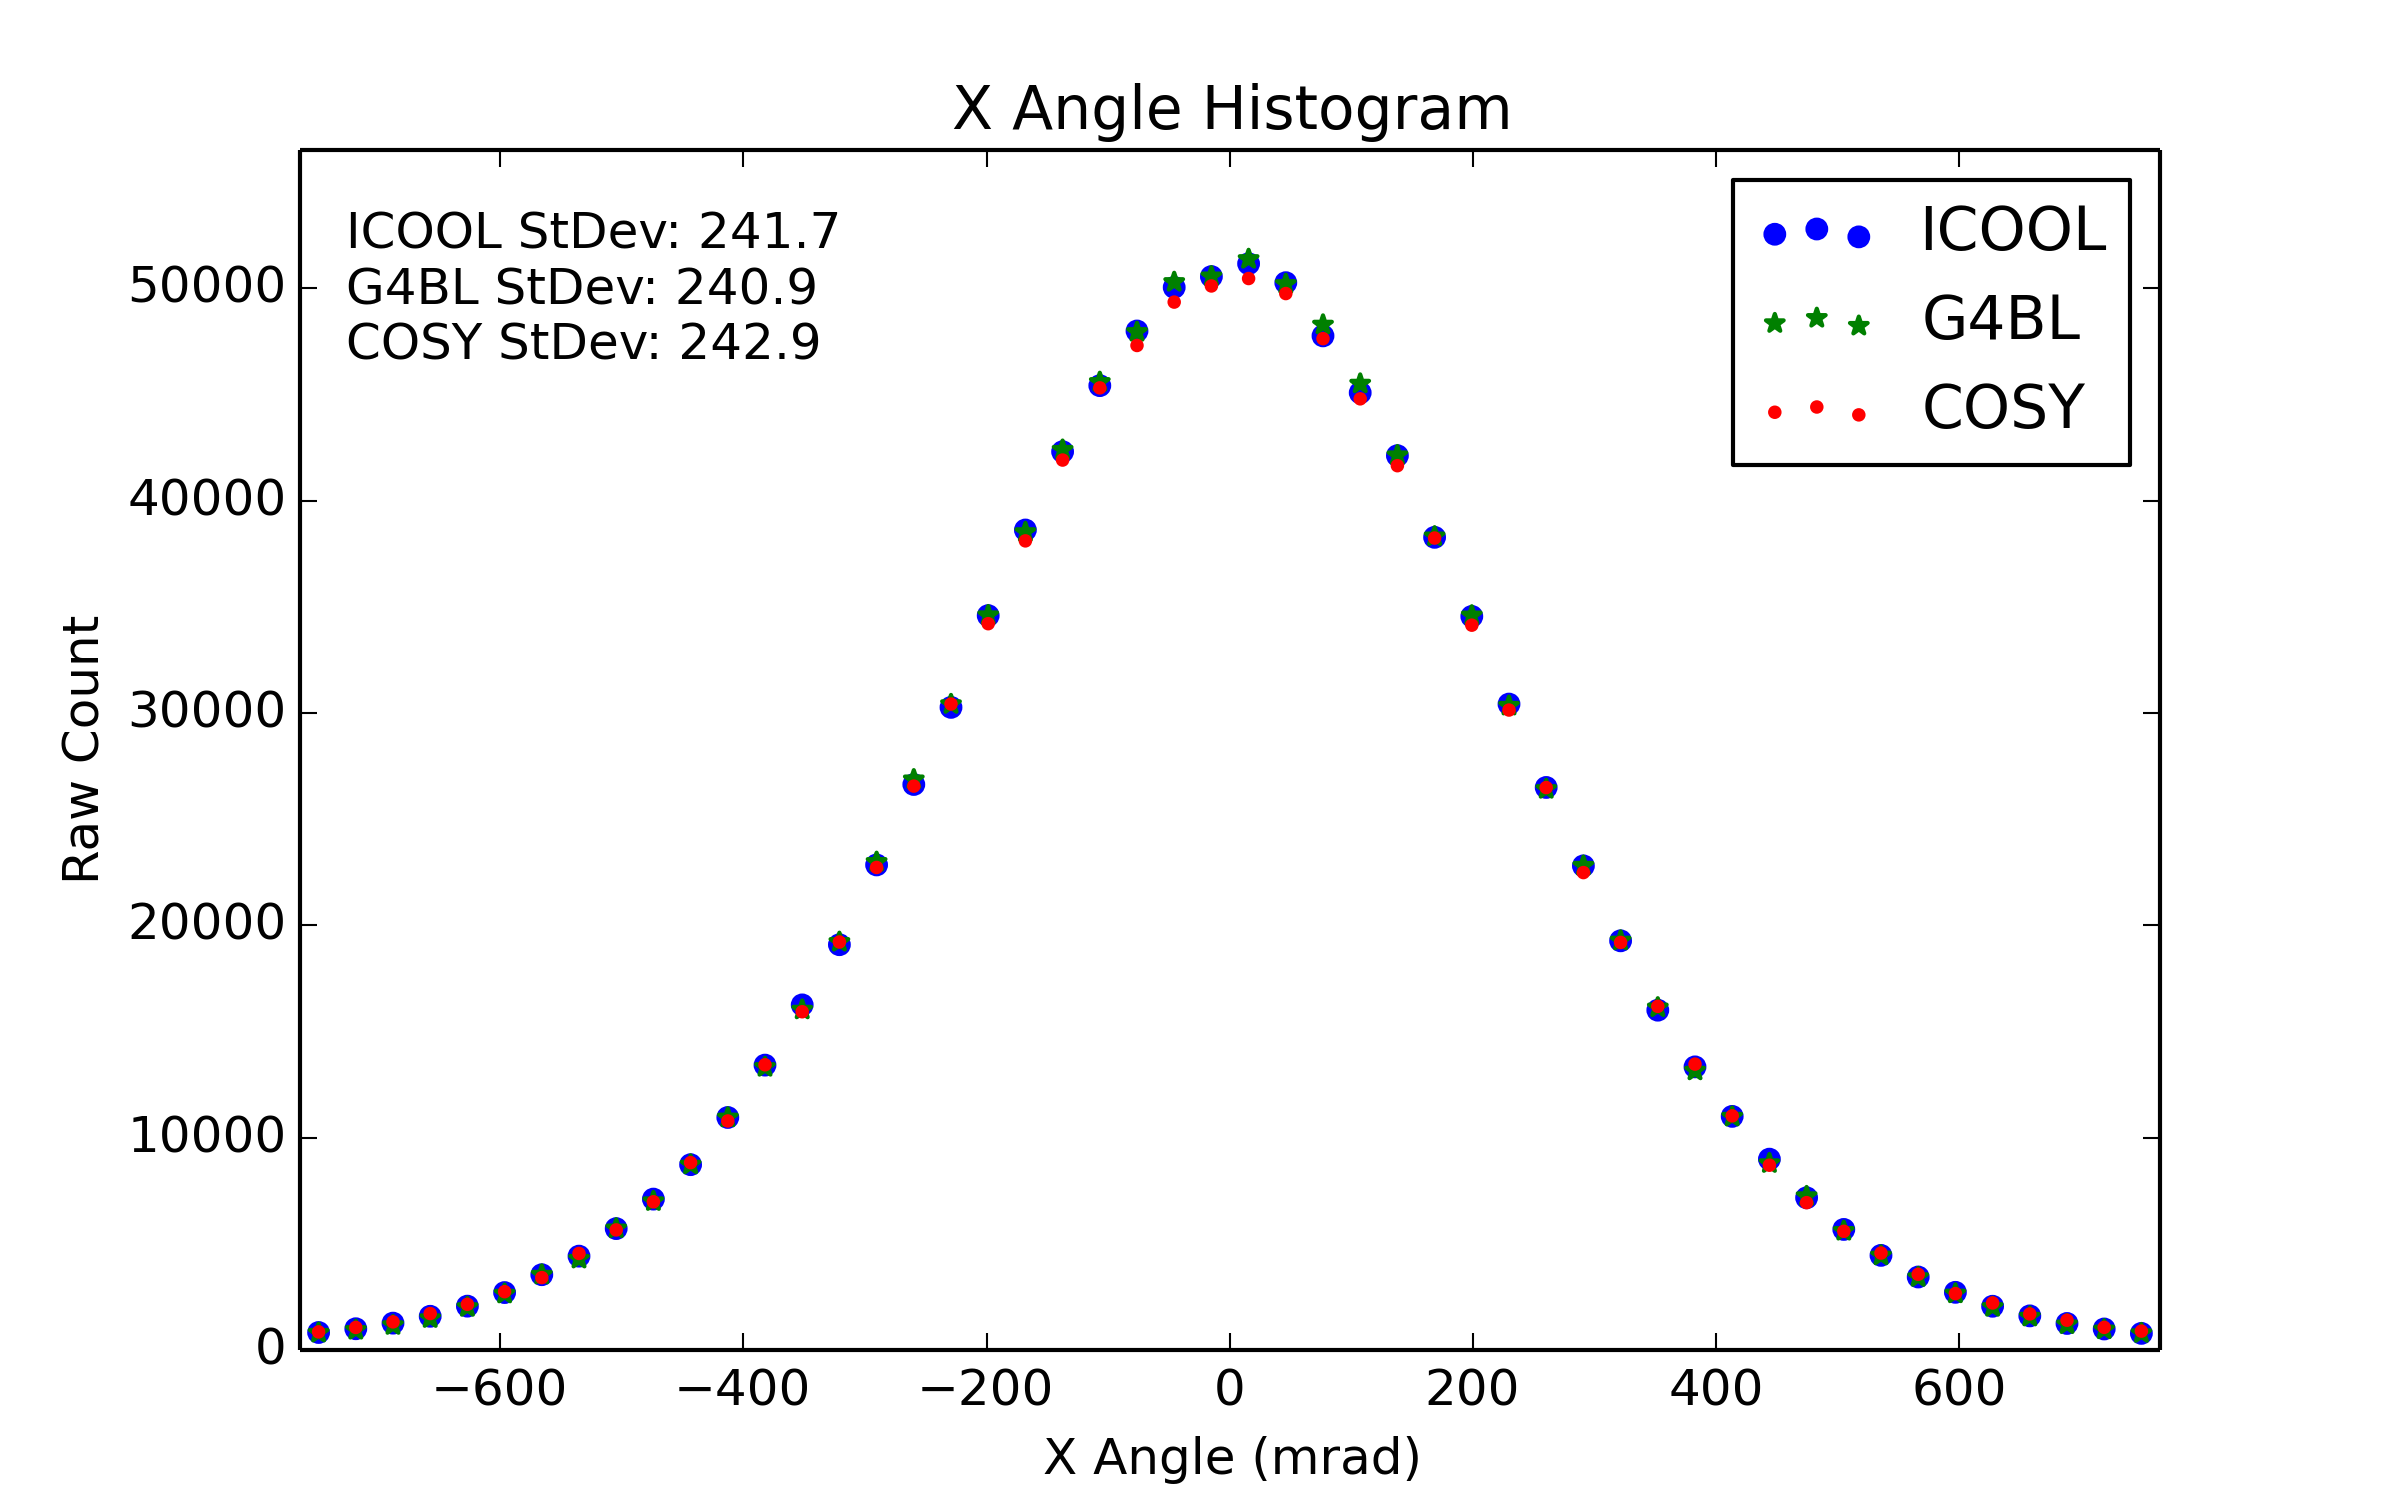
\includegraphics[width=\textwidth]{MICE data/LiH/px} 
  \caption{MICE Step IV $x$ angle results for 65 mm of lithium hydride.}
  \label{fig:mice_lih_xangle}
\end{figure}

\begin{figure}[H]
  \centering
    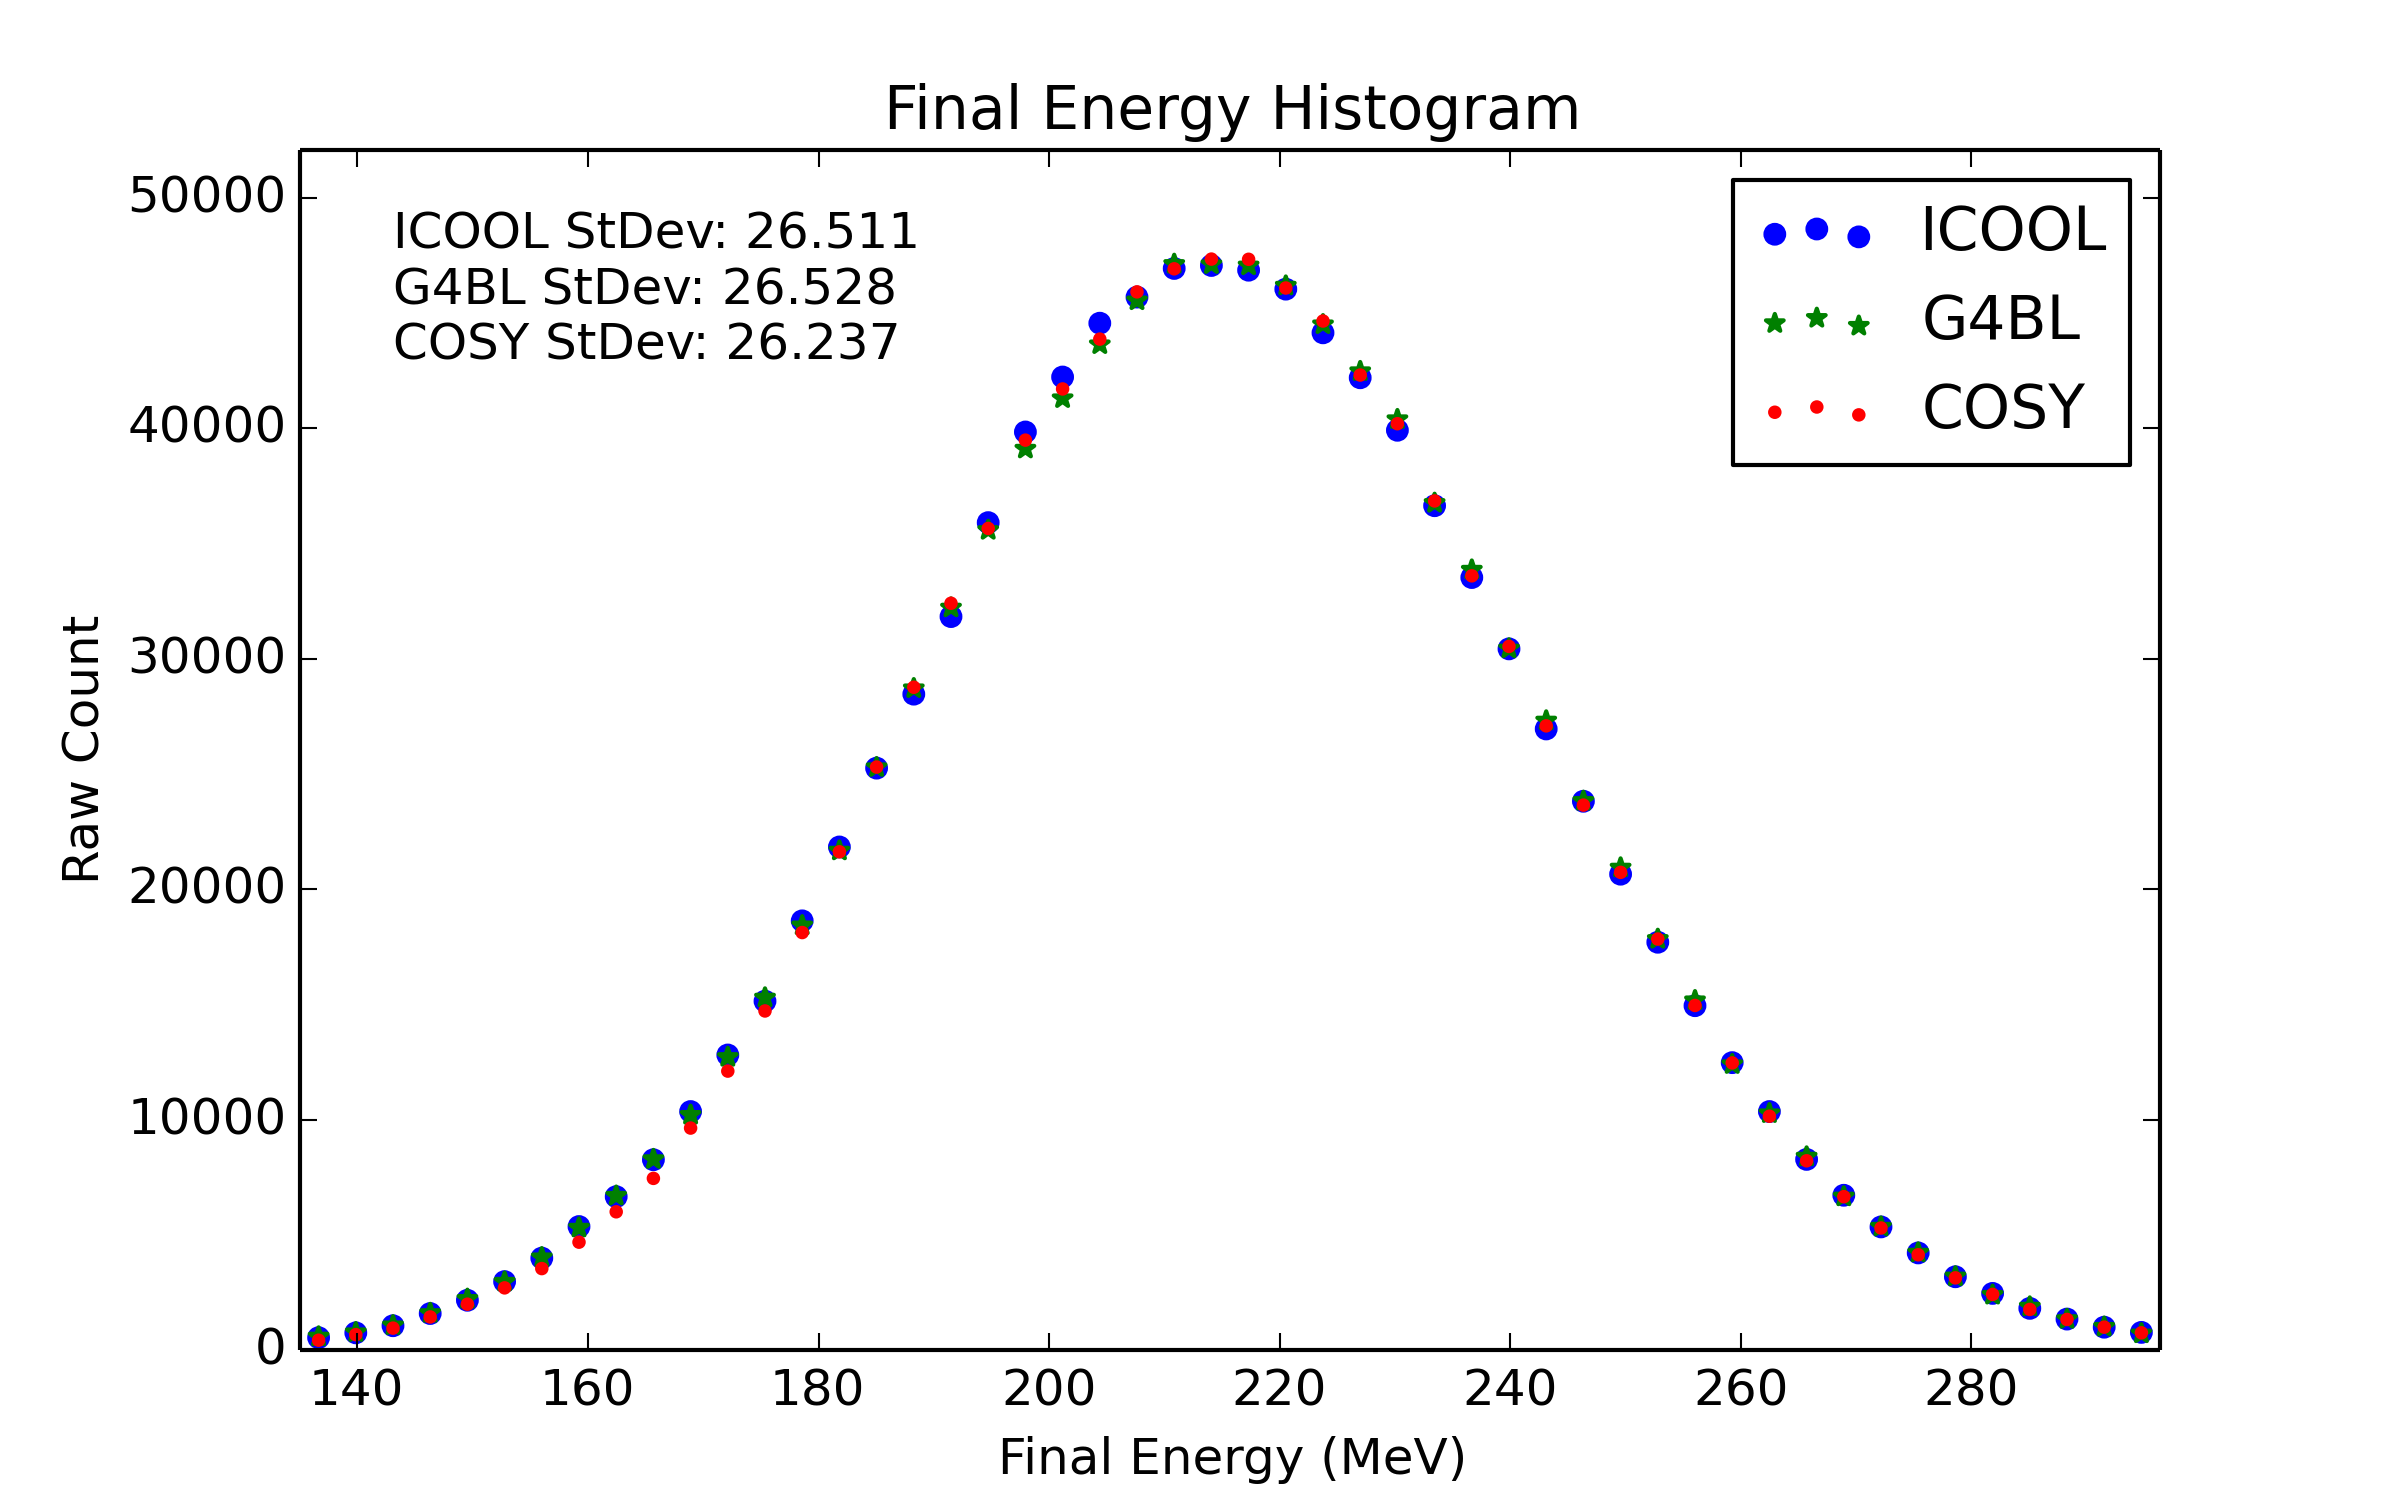
\includegraphics[width=\textwidth]{MICE data/LiH/e} 
  \caption{MICE Step IV final energy results for 65 mm of lithium hydride.}
  \label{fig:mice_lih_energy}
\end{figure}

\Subsection{Step Size Effects}\label{ssc:step_size_effects}
Several step sizes were tested in COSY to ensure optimal efficiency. While it was found that the results are fairly consistent regardless of step size, the results are discussed here.

For the upstream section ($-2.45105$ m to $-0.35/2$ m) of MICE liquid hydrogen lattice, it was found that COSY operated sufficiently well at order 5 and with 100 steps in the simulation.

To study this step size dependence, $10^5$ particles from the initial distribution found in Table~\ref{tbl:MICE_initial_distribution_parameters} were propagated through the upstream coils. Table~\ref{tbl:mice_step_size_upstream} shows the effect of changing the step size for the upstream section.

\begin{table}
\caption*{\textbf{Step Size Dependence for Upstream Section}}
\begin{center}
\begin{tabularx}{\textwidth}{ccccccc}
\hline \hline
Parameter & 3@50 & 3@100 & 5@100 & 9@100 & G4Beamline & ICOOL\\
\hline
$\sigma_x$ (mm): & 46.44 & 46.47 & 46.94 & 46.96 & 46.80 & 46.80\\
$\sigma_{\theta_x}$ (mrad): & 91.7 & 91.6 & 92.4 & 92.5 & 92.8 & 92.8\\
Computational time (s): & 8.3 & 10.2 & 22.4 & 182 & 366 & 25\\
\hline
\end{tabularx}
\end{center}
\caption[Step size dependence for the upstream section of MICE Step IV lattice.]{Step size dependence for the upstream section of MICE Step IV lattice for $10^5$ muons. The notation for COSY is [order] @ [number of steps].}
\label{tbl:mice_step_size_upstream}
\end{table}

For all four COSY cases, the discrepancy w.r.t. G4Beamline is  $<$1\% for the transverse position component and on the order of 1\% for the angular component. 5th order at 100 steps was selected as ``best'' because of the increased agreement with both ICOOL and G4Beamline when compared to both 3@50 and 3@100 (particularly for the angular component). Moreover, 5@100 gives similar results as 9@100 but with drastically decreased computational time. While 5@100 requires over double the computational time of 3@100, the computational time for 5@100 is still acceptable.

Results of the upstream simulation can be seen in Figures \ref{fig:upx} and \ref{fig:uppx}. There is good agreement between ICOOL, G4Beamline, and COSY. Note that ICOOL agrees with G4Beamline extremely well because ICOOL is using a field map generated by G4Beamline (as was discussed in Section~\ref{ssc:miceResults}, MICE results section).

\begin{figure}[H]
  \centering
    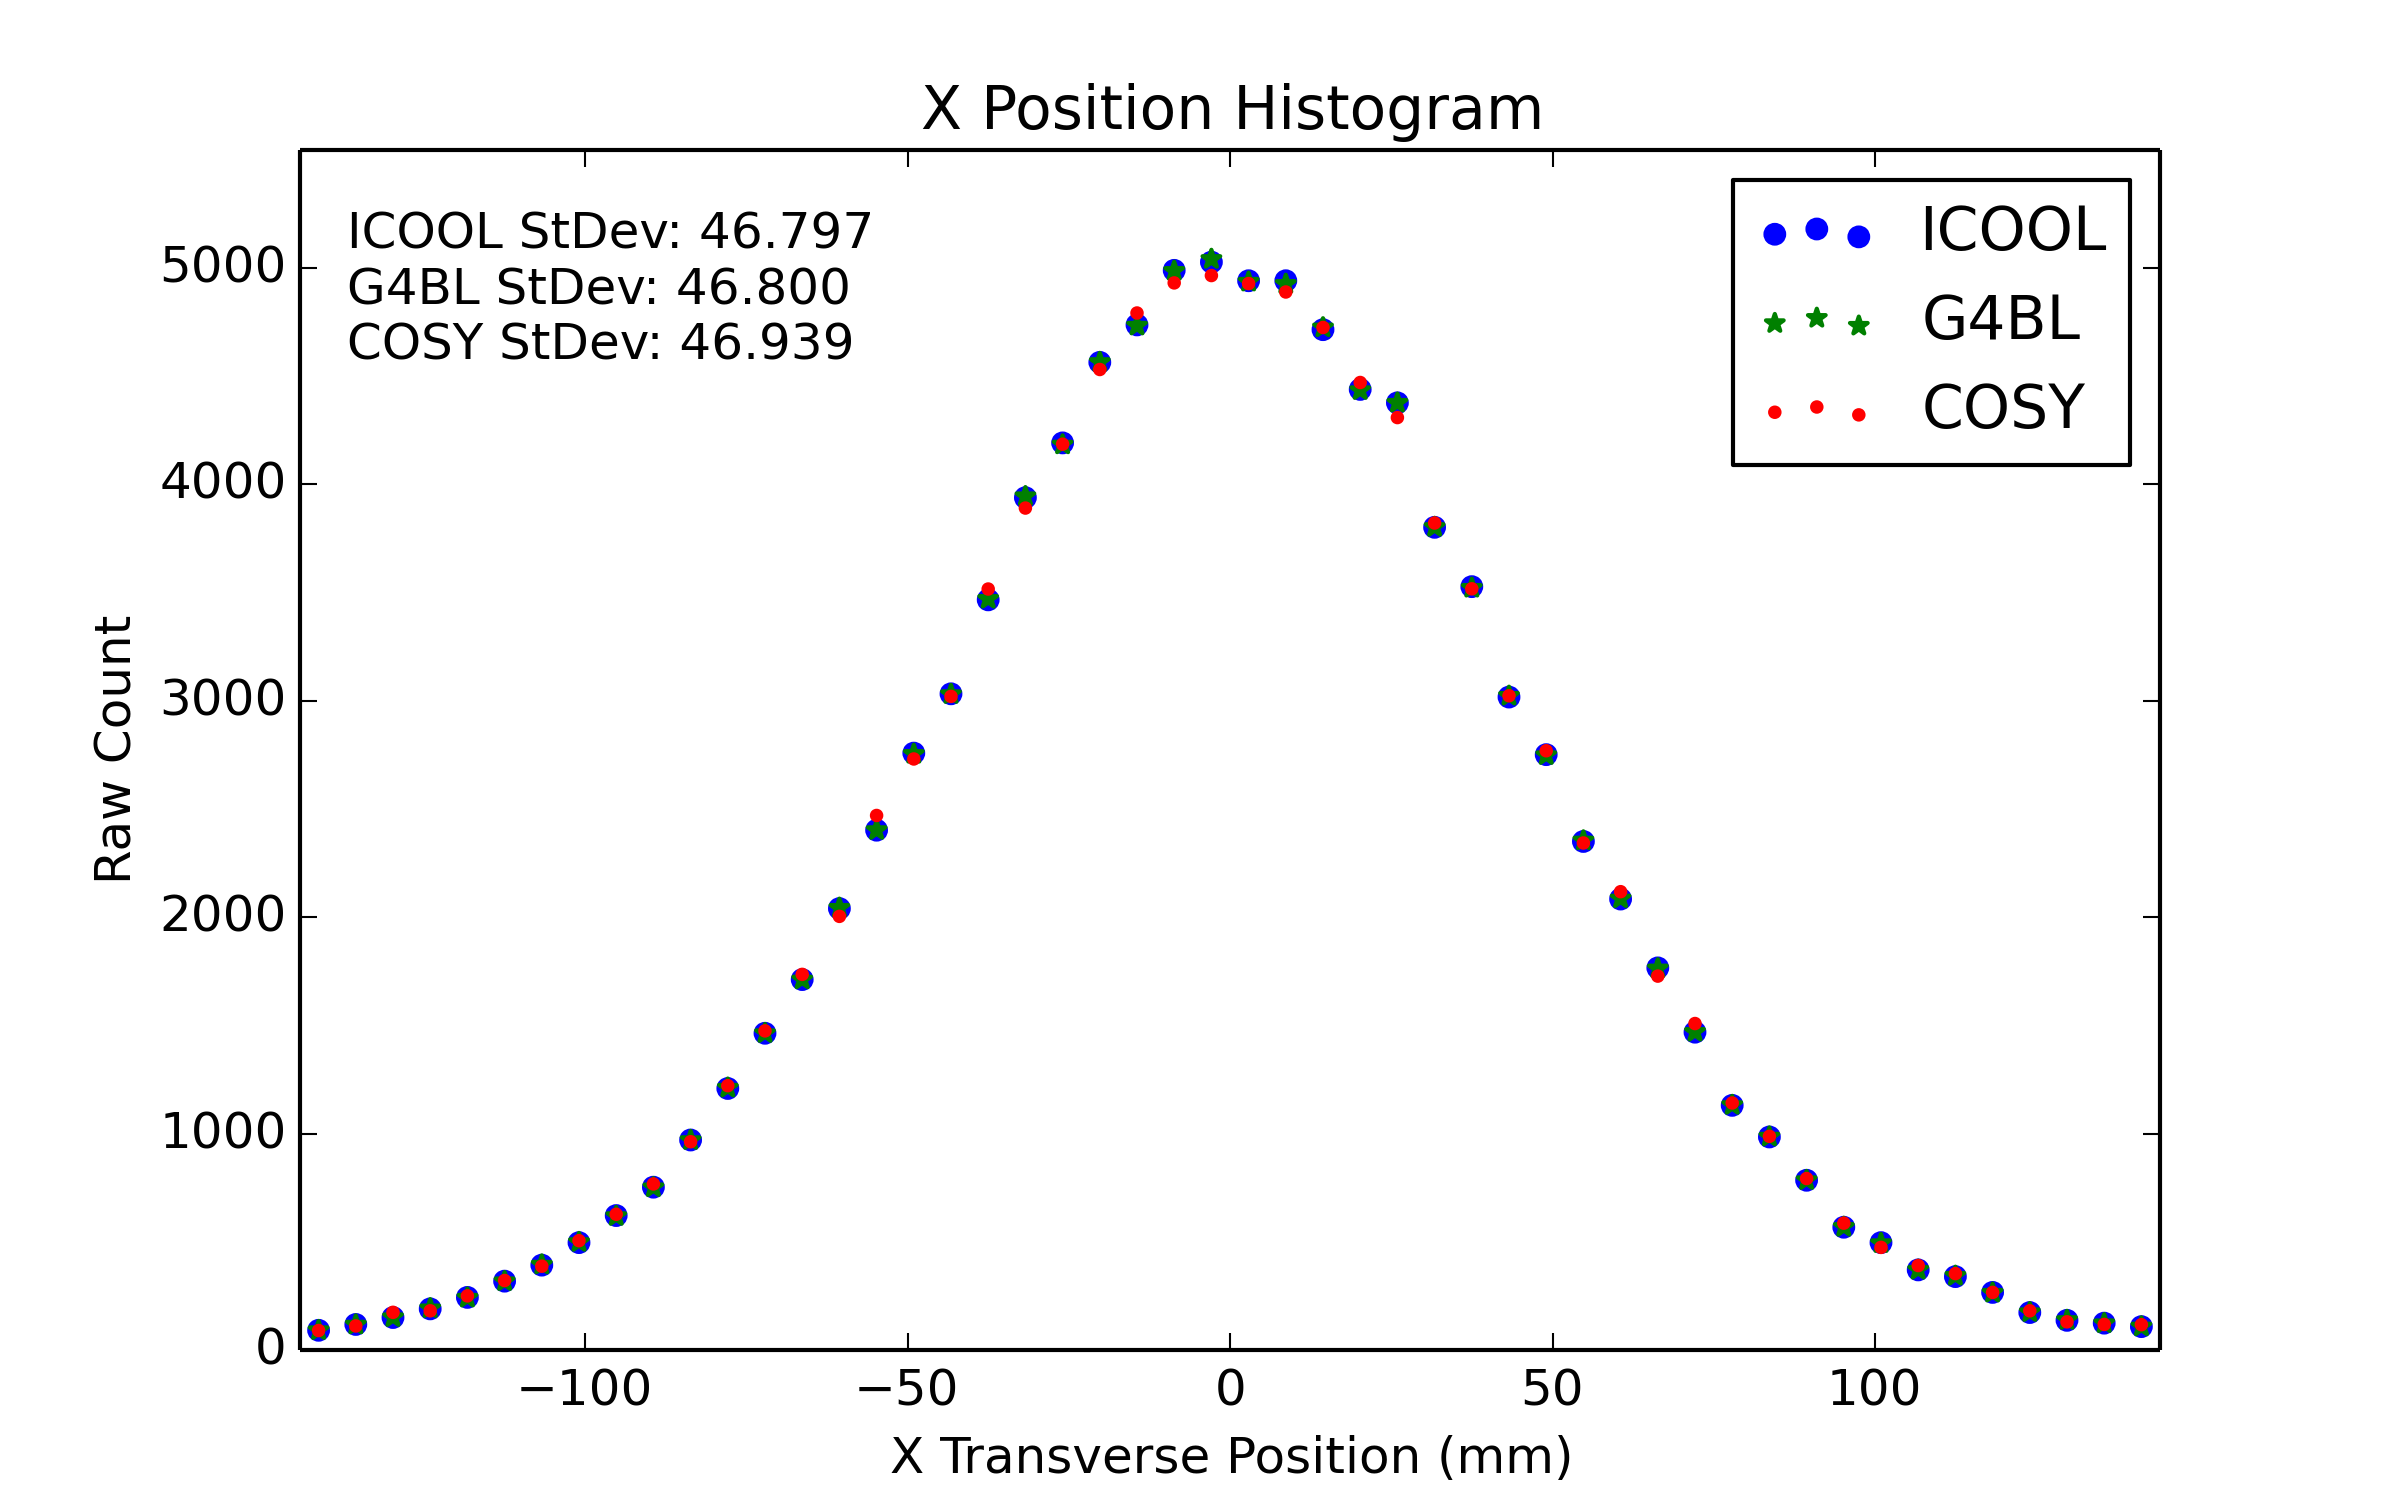
\includegraphics[width=0.7\textwidth]{MICE data/upstream/x} 
  \caption{Upstream simulation results for $x$ at 5th order and 100 steps.}
  \label{fig:upx}
\end{figure}

\begin{figure}[H]
  \centering
    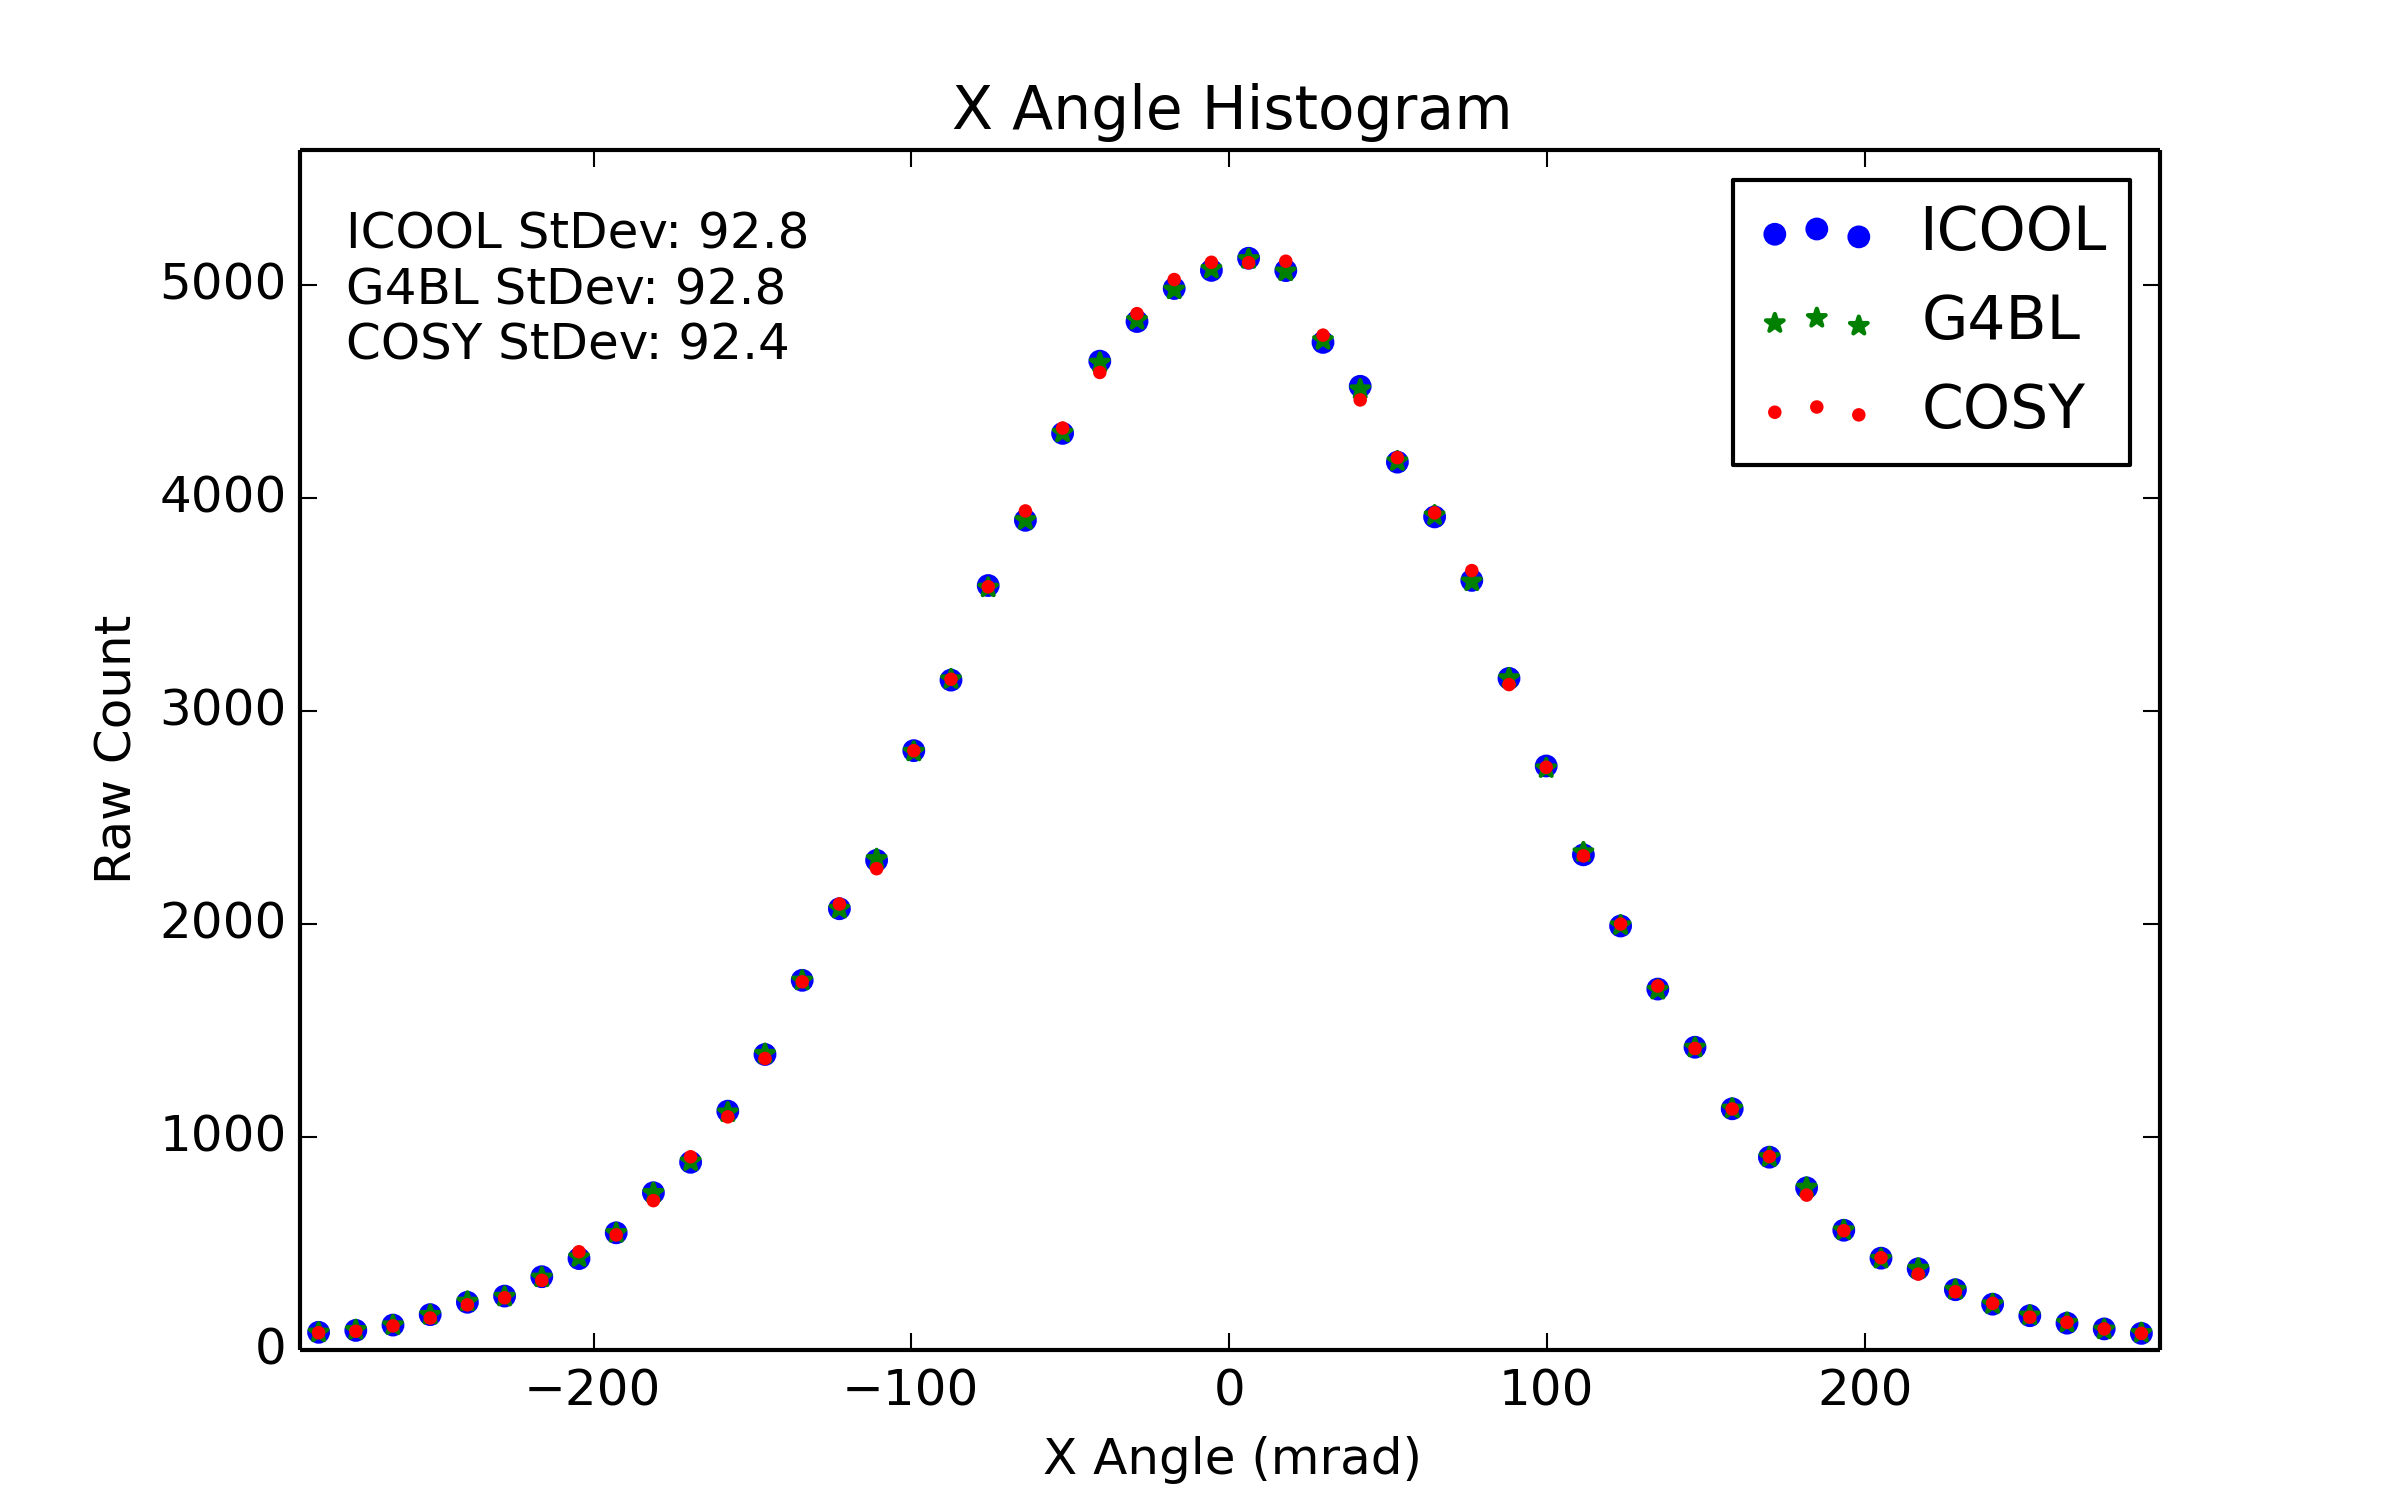
\includegraphics[width=0.7\textwidth]{MICE data/upstream/px} 
  \caption{Upstream simulation results for $\theta_x$ at 5th order and 100 steps.}
  \label{fig:uppx}
\end{figure}

For the absorber-coil section of MICE liquid hydrogen lattice ($-$0.35/2 to 0.35/2), it was found that a 10 mm step size was sufficient to approximate the superposition of the absorber and coils. To study this step size dependence, $10^5$ particles from the initial distribution found in Table~\ref{tbl:MICE_initial_distribution_parameters} were propagated through the 350 mm liquid hydrogen flat absorber. This simulation took the surrounding magnetic fields into account. Table~\ref{tbl:mice_step_size_ac} shows the effect of changing the step size for the absorber-coil section only. The step size in ICOOL was 1 mm.

\begin{table}
\caption*{\textbf{Step Size Dependence for Absorber-Coil Section (Liquid Hydrogen)}}
\begin{center}
\begin{tabularx}{\textwidth}{cccccc}
\hline \hline
Parameter &1 mm & 10 mm & 50 mm & G4Beamline & ICOOL\\
\hline
$\sigma_x$ (mm): & 51.29 & 51.31 & 51.24 & 50.42 & 50.43\\
$\sigma_{\theta_x}$ (mrad): & 203.6 & 203.8 & 204.5 & 202.0 & 202.5\\
%$\sigma_y$ (mm): & 51.18 & 51.20 & 51.19 & 50.39 & 50.38\\
%$\sigma_{\theta_y}$ (mrad): & 203.0 & 203.2 & 203.8 & 201.9 & 202.4\\
$\sigma_E$ (MeV): & 26.66 & 26.66 & 26.64 & 26.67 & 26.67\\
Computational time (s): & 240.9 & 27.8 & 10.8 & 257.8 & 20.0\\
\hline
\end{tabularx}
\end{center}
\caption[Step size dependence for the absorber-coil section of MICE Step IV lattice for liquid hydrogen.]{Step size dependence for the absorber-coil section of MICE Step IV lattice for $10^5$ muons passing through 350 mm of liquid hydrogen.}
\label{tbl:mice_step_size_ac}
\end{table}

The discrepancy of COSY w.r.t. G4Beamline is on the order of 1\% for the position component and $<$1\% for the other components. Results of the absorber-coil simulation can be seen in Figures \ref{fig:acx}-\ref{fig:ace}. There is good agreement between ICOOL, G4Beamline, and COSY.

\begin{figure}[H]
  \centering
    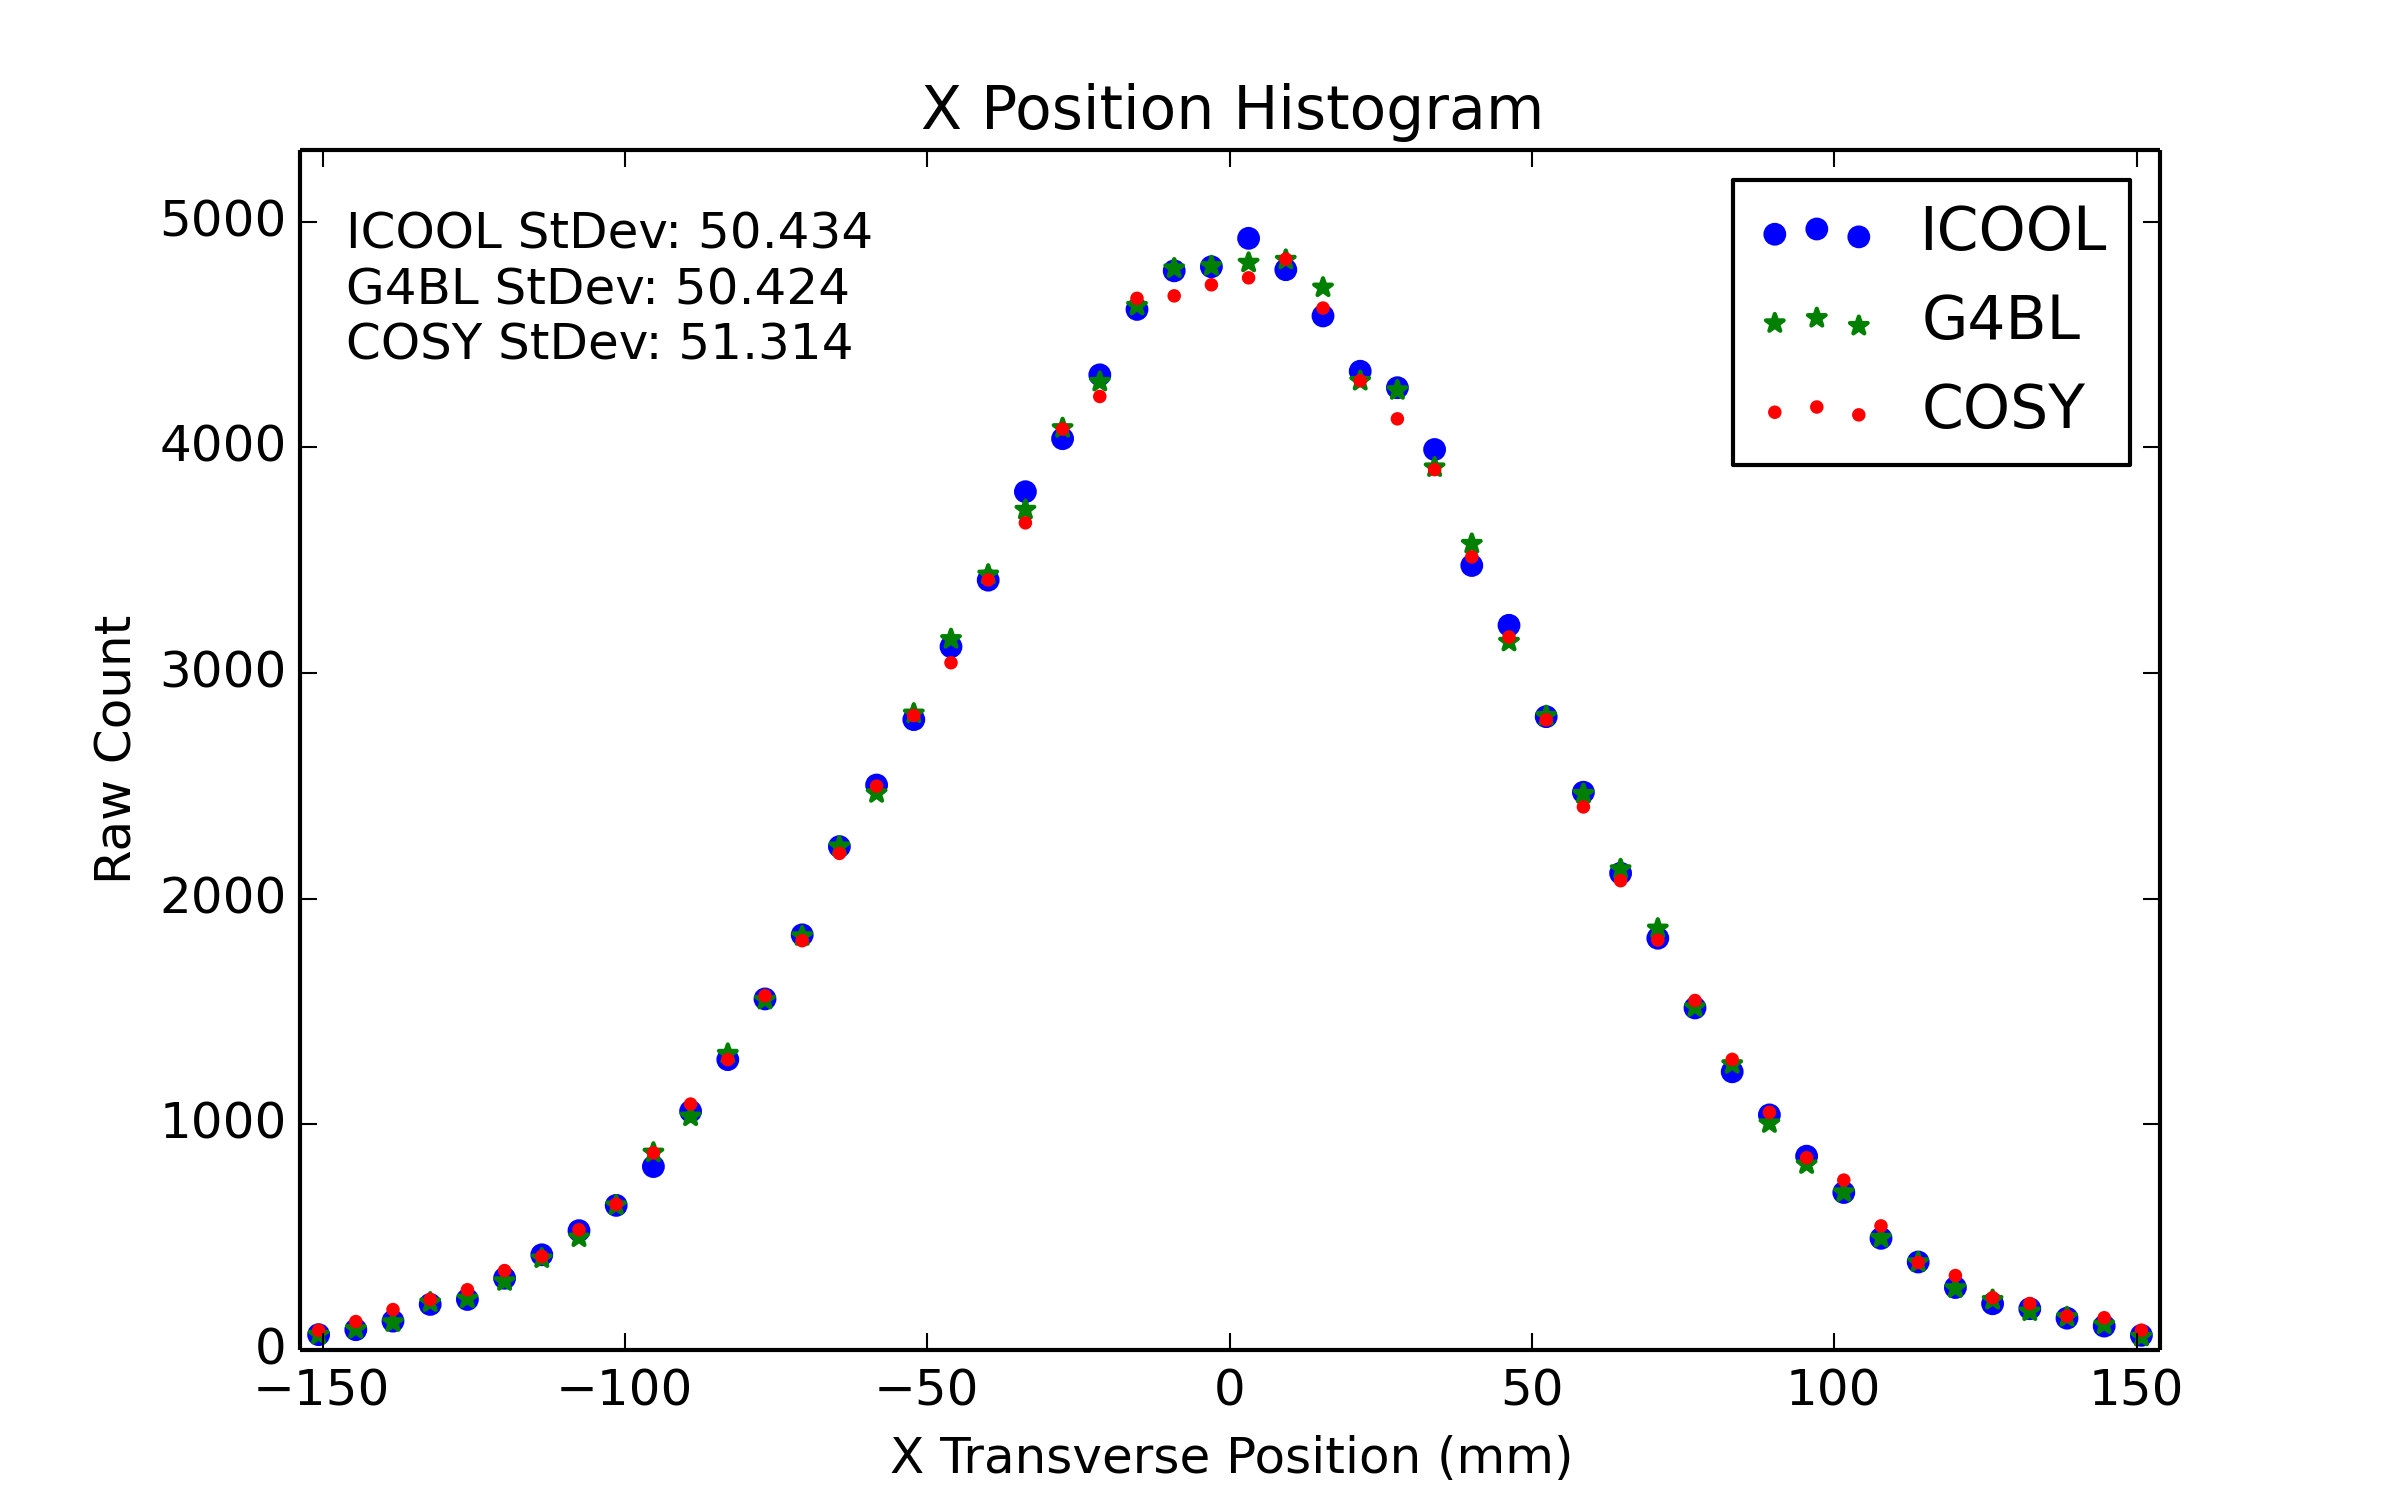
\includegraphics[width=0.7\textwidth]{MICE data/absorber coils/x} 
  \caption{Absorber-coil simulation results for $x$ at a step size of 10 mm.}
  \label{fig:acx}
\end{figure}

\begin{figure}[H]
  \centering
    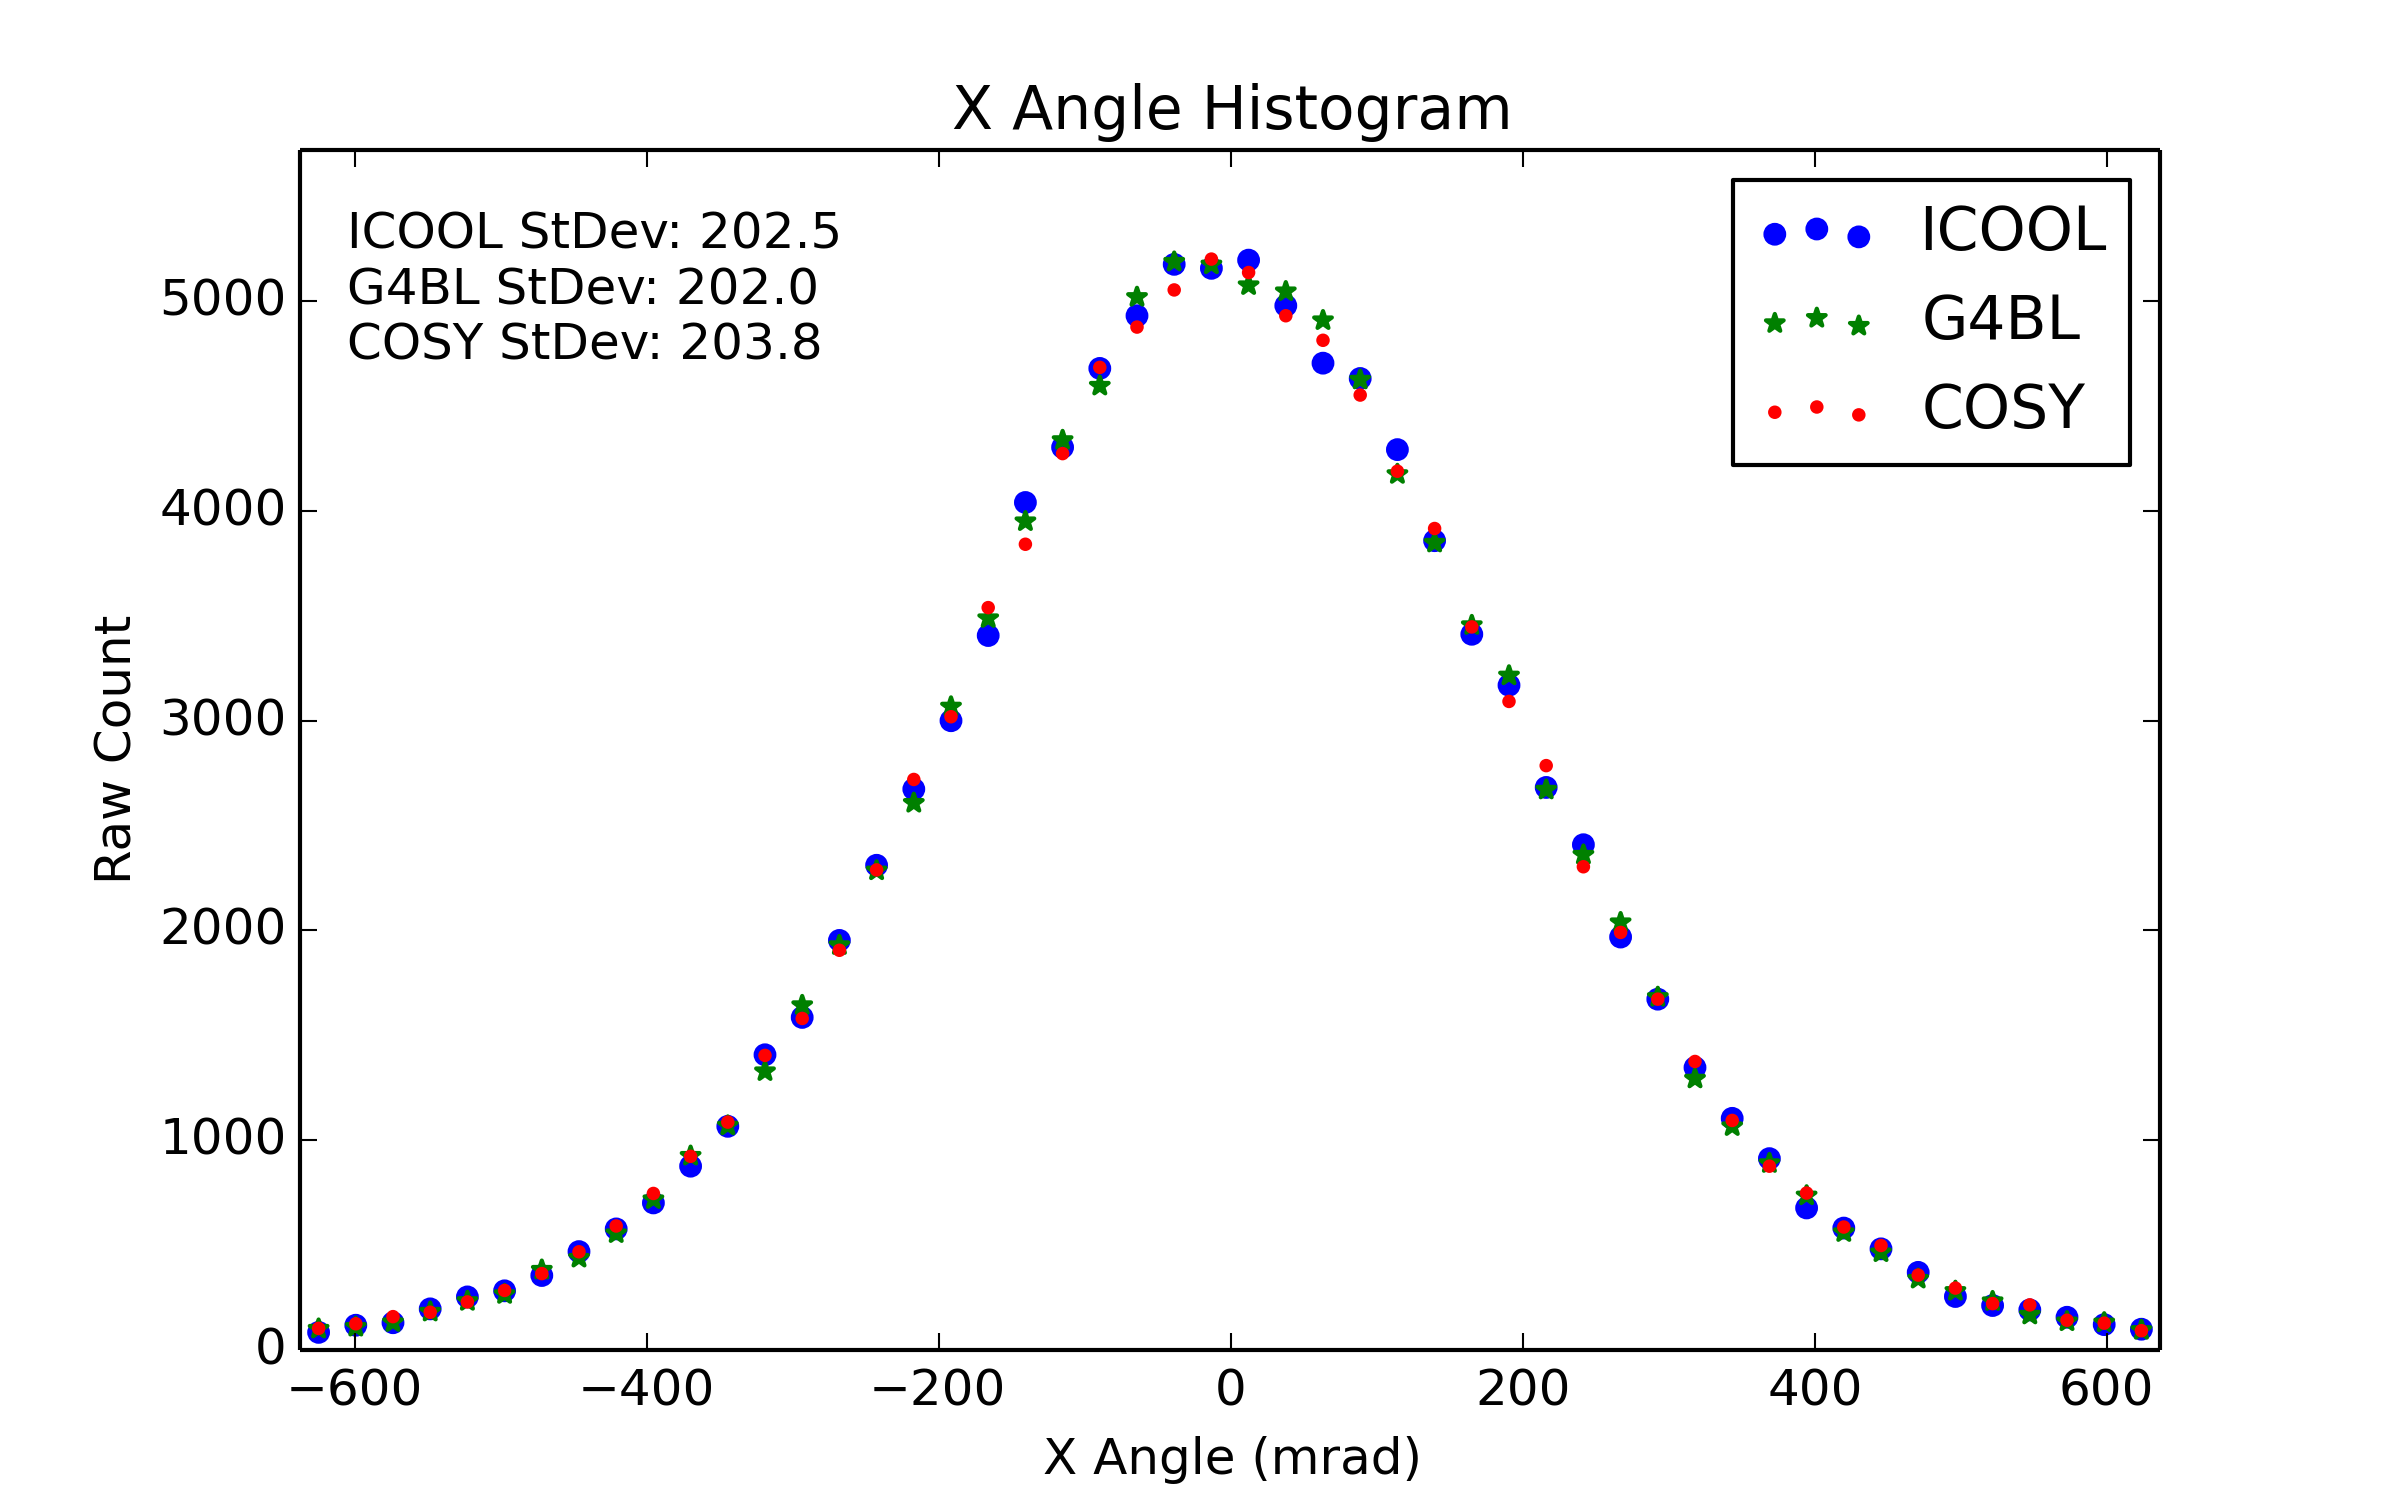
\includegraphics[width=0.7\textwidth]{MICE data/absorber coils/px} 
  \caption{Absorber-coil simulation results for $\theta_x$ at a step size of 10 mm.}
  \label{fig:acpx}
\end{figure}

\begin{figure}[H]
  \centering
    \includegraphics[width=0.7\textwidth]{MICE data/absorber coils/e} 
  \caption{Absorber-coil simulation results for the final energy at a step size of 10 mm.}
  \label{fig:ace}
\end{figure}

Since the downstream coils are very similar to the upstream coils, the downstream coils were not tested separately. For the full simulation in Section~\ref{ssc:miceResults}, the downstream order and step size were identical to the upstream order and step size.

\Section{Summary}\label{sec:summary}

In summary, new simulation tools for muon ionization cooling have been added to COSY Infinity for particle-by-particle propagation. The energy straggling, multiple scattering, transverse position, and time-of-flight models were developed from first principles. The algorithms implemented have been modified via empirical fit to MuScat \cite{muscat} while keeping reasonable agreement with G4Beamline. Fitted with this new software, COSY has simulated one of the current muon ionization cooling efforts, MICE Step IV \cite{mice}, yielding good agreement with both ICOOL and G4Beamline. The code developed in this work is accurate, fast, and user-friendly.